% This is samplepaper.tex, a sample chapter demonstrating the
% LLNCS macro package for Springer Computer Science proceedings;
% Version 2.21 of 2022/01/12

\documentclass[runningheads,a4paper]{llncs}
% If you use the hyperref package, please uncomment the following two lines
% to display URLs in blue roman font according to Springer's eBook style:
%\usepackage{color}
%\renewcommand\UrlFont{\color{blue}\rmfamily}
%\urlstyle{rm}

% PREAMBLE
\usepackage[utf8]{inputenc}
\usepackage{amsfonts}
\usepackage{amssymb}
\usepackage{circuitikz}
\usepackage{cite}

\usepackage{xcolor}
\usepackage[
	n,
	operators,
	advantage,
	sets,
	adversary,
	landau,
	probability,
	notions,	
	logic,
	ff,
	mm,
	primitives,
	events,
	complexity,
	asymptotics,
	keys]{cryptocode}
\usepackage{enumitem}
\setlist{nosep}
\usepackage[hidelinks]{hyperref}
%\usepackage{todonotes}

\usepackage{lscape}
\usepackage{mathtools}

% MACROS

% ~~ General

%\DeclareMathOperator*{\argmax}{arg\,max}
%\DeclareMathOperator*{\argmin}{arg\,min}

\renewcommand{\secpar}{\lambda}
\renewcommand{\secparam}{1^\lambda}


% ~~ Formatting
\definecolor{hybrid}{HTML}{0076BA}

\usepackage{caption} 
\captionsetup[table]{skip=10pt}

\begin{document}
%
\title{Bruisable Onions: Anonymous Communication in the Asynchronous Model}
%
%\titlerunning{Abbreviated paper title}
% If the paper title is too long for the running head, you can set
% an abbreviated paper title here
%
\author{
Megumi Ando\inst{1}\orcidID{0000-0002-4639-9163}\index{Ando, Megumi}
\and
Anna Lysyanskaya\inst{2}\index{Lysyanskaya, Anna}%\orcidID{1111-2222-3333-4444} 
\and
Eli Upfal\inst{2}\orcidID{0000-0002-9321-9460}}\index{Upfal, Eli}
%
\authorrunning{M. Ando et al.}
% First names are abbreviated in the running head.
% If there are more than two authors, 'et al.' is used.
%
\institute{
Tufts University, Medford MA, USA 
\and
Brown University, Providence RI, USA
}
%
\maketitle              % typeset the header of the contribution
%
\begin{abstract}
%The abstract should briefly summarize the contents of the paper in 150--250 words.
In onion routing, a message travels through the network via a series of intermediaries, wrapped in layers of encryption to make it difficult to trace.
%
Onion routing is an attractive approach to realizing anonymous channels because it is simple and fault tolerant.
%
Onion routing protocols provably achieving anonymity in realistic adversary models are known for the synchronous model of communication so far.
%
In this paper, we give the first onion routing protocol that achieves anonymity in the asynchronous model of communication.
%
The key tool that our protocol relies on is the novel cryptographic object that we call \textit{bruisable} onion encryption.
%
The idea of bruisable onion encryption is that even though neither the onion's path nor its message content can be altered in transit, an intermediate router on the onion's path that observes that the onion is delayed can nevertheless slightly damage, or bruise it.  An onion that is chronically delayed will have been bruised by many intermediaries on its path and become undeliverable.  This prevents timing attacks and, as we show, yields a provably secure onion routing protocol in the asynchronous setting. 
%\keywords{First keyword  \and Second keyword \and Another keyword.}
\end{abstract}
%
%
%
\newcommand{\parties}{\mathsf{Parties}}
\newcommand{\keygen}{\mathsf{KeyGen}}
\newcommand{\formonion}{\mathsf{FormOnion}}
\newcommand{\proconion}{\mathsf{PeelOnion}}
\newcommand{\proconionhelper}{\mathsf{PeelOnionHelper}}
\newcommand{\bruiseonion}{\mathsf{BruiseOnion}}
\newcommand{\polylog}{\mathsf{polylog}}
\newcommand{\early}{\mathsf{early}}
\newcommand{\late}{\mathsf{late}}
\newcommand{\recipient}{\mathsf{Recipient}}
\newcommand{\Bad}{\mathsf{Bad}}

%\newcommand{\eli}[1]{\textcolor{blue}{Eli: #1]}}
\section{Introduction}
 
The ability to communicate anonymously is an increasingly vital component of digital life and citizenship.
From Iranian protesters wishing to safely to inform the world what is happening in the streets of Tehran, to Russian citizens trying to communicate with outside media, anonymity gives people all over the world a chance to exercise their fundamental rights without fear of repercussions.  
%
Practical tools such as Tor~\cite{tor} (i.e., ``The onion router,''  inspired by Chaum's onion routing idea~\cite{Chaum81} described below) or VPNs have a lot of room for improvement.  Both are easily blocked, and neither guarantees privacy even from the network adversary (e.g., a standard model for a resourceful ISP- or AS-level adversary)~\cite{SP:MurDan05, SEVL+15, WSJCM18, gizmodo}. 

A communications protocol is anonymous~\cite{ando2019complexity} if for any pair of input vectors $(\sigma_0, \sigma_1)$ that differ only on the inputs and outputs\footnote{Here, by ``output" of a party $P$ we mean a set of messages $\{m\}$ such that some party $P'$ receives $(m,P)$ as part of its input.  I.e. $P'$ intends to send $m$ to $P$. } of honest parties (e.g., Alice sends to Bob in $\sigma_0$ and to Charlie in $\sigma_1$), the adversary (whose capabilities vary depending on the adversarial model) %; of particular interest is the adversary that controls the network and a subset of participants) 
cannot tell from interacting with the honest nodes in a protocol run whether the input was $\sigma_0$ or $\sigma_1$.\footnote{Alternative definitions of anonymity exist~\cite{BKMMM,KuhnBSJS19}, but we will be referring to the standard cryptographic definition here.}  

% Chaum
% all our papers 
% Kuhn et al. with replies
% breaking and paritally fixing 
% vuvuzela? stadium?
The goal of research on onion routing~\cite{Chaum81,JC:Chaum88,C:CamLys05,vuvuzela,ICALP:AndLysUpf18,SP:KuhBecStr20,ando2019complexity,TCC:AndLys21,AC:KHRS21,TCC:ACLM22} is to achieve this definition in the presence of a malicious adversary corrupting a fraction of the participants, with a communication- and computation- efficient, fault-tolerant and decentralized protocol.   
In an onion routing protocol, to send a message to Bob, Alice first picks a sequence of intermediary parties $I_1, \dots, I_{\ell-1}$ and then forms a layered cryptographic object called an onion using the message and the routing path $(I_1, \dots, I_{\ell-1}, \text{Bob})$. % (and the public keys of the nodes associated with the path). 
Alice then sends the onion to the first intermediary $I_1$ on the routing path who peels off just the outermost layer of the onion (i.e., processes the onion) and sends the peeled onion~$O_2$ to the next party $I_2$ on the routing path, $I_2$ peels $O_2$ and sends the peeled onion $O_3$ to $I_3$, and so on. This procedure continues until Bob receives the message %(the ``innermost onion'') 
from Alice. 

In an onion routing protocol that uses standard cryptographic onions~\cite{C:CamLys05}, % (as defined by Camenisch and Lysyanskaya in~\cite{C:CamLys05}), 
even a powerful adversary who can corrupt (and ``look into'' or even control) some of the parties cannot link an honest party's incoming onion to its outgoing onion. This lack of transparency allows for shuffling onions when they are batch-processed at an honest party~\cite{STOC:RacSim93,FC:BerFiaTas04,iwanik2005duo, ICALP:AndLysUpf18}.%\todo{add refs for papers analyzing this}  %When onions are processed in synchronous stages, onion routing protocols achieving anonymity from the network adversary and also, in some cases, from the active adversary that corrupts some of the participants have been studied~\cite{}.


% State of the art 
\paragraph{Technical challenge: asynchronous onion routing.}
%Currently known solutions either offer limited anonymity (e.g., \cite{reiter1998crowds, clarke2001freenet, tor, piotrowska2017loopix})
%(these include Crowds [ref], Freenet [ref], I2P [ref], Tor [ref], and Loopix [ref]) 
%or are impractical (e.g., \cite{JC:Chaum88, STOC:RacSim93, SP:CooBir95, BIK+}). 
%An an example of the former, Tor is an onion routing protocol currently in use by millions of users~\cite{tor}, which, while clearly practical, is vulnerable to traffic analysis attacks~\cite{SP:MurDan05, SEVL+15, SP:SEFCM17, gizmodo}. 
%On the theory side, researchers have known about anonymous methods that are clearly not practical~\cite{JC:Chaum88, STOC:RacSim93, SP:CooBir95, SP:CorBonMaz15, BIK+}. 
%\todo{Commented out refs to older, less directly relevant work}
In recent years, several protocols were presented as provably secure yet practical solutions~\cite{SP:CorBonMaz15, vuvuzela, stadium, atom, ICALP:AndLysUpf18, ando2019complexity}. However, all these protocols' security analysis requires synchronous communication. 
In the synchronous communications setting, time progresses in rounds, and message transmissions are lossless and instantaneous. While modeling communications in this way makes designing and analyzing anonymity protocols more tractable, it is somewhat of a cheat. Currently deployed anonymity protocols, such as Tor~\cite{tor} and Loopix~\cite{piotrowska2017loopix}, are known to be vulnerable to traffic analysis attacks~\cite{SP:MurDan05, SEVL+15, WSJCM18, attarian2023mixflow}
that exploit the asynchronous nature of communication in the real world.

%in which anonymity is broken by relating the bitrate from the sender to that on the receiving end. By modeling message packets (onions, in our case) as arriving as intended and without delays, we abstract away some of the traffic metadata used to successfully conduct attacks in the real world. 

Constructing a solution for the asynchronous setting is challenging because the adversary can easily influence the traffic flow, for example, by mounting a BGP interception attack~\cite{SEVL+15}, so that a targeted message arrives with an expected and observable delay. (See Section~\ref{sec:contribitions} for an example of a timing attack on a preciously known solution.) The adversary can do this even if the onions are batch-processed and even if we are willing to pay a cost by increasing the latency and/or volume of dummy traffic. As we explain below, this attack method breaks the anonymity of every known protocol designed and proven secure for the synchronous setting; this is a problem that is not trivially fixable by using sychronizers (which assume no failures) or clock synchronization algorithms (which guarantees that most if not all of the honest parties are synchronized)~\cite{lynch1996distributed}. %\todo{Confirm this://www.mpi-inf.mpg.de/fileadmin/inf/d1/teaching/summer18/TKDS/lec4.pdf. Add refs.}
In this paper, we present the first \textbf{provably anonymous} onion routing protocol for the asynchronous communications setting. %\todo{I changed ``the first provably anonymous protocol'' to ``a provably anonymous protocol.''}
%\eli{If we say "In this paper, we present a provably anonymous protocol" then why is it interesting? Why is it an improvement of previous work? In the Abstract we wrote "In this paper, we give the first onion routing protocol that achieves anonymity in the asynchronous model of communication". Is this a correct statement?}

%\begin{itemize} 

%\item Recent advances in provable anonymity. List them. But these are only for the synchronous setting. 

%\item Real world is asynchronous. 

%\item But current asynchronous approaches are provably not secure: Tor, Poisson mixing (Loopix) isn't anonymous. 
%    \begin{itemize}
%    \item \url{https://eprint.iacr.org/2023/199.pdf}
%    \end{itemize}

%\item Describe $\Pi_a$ (most practical of the known provably anonymous protocols)

%\item Explain the timing attack. 

%\item Attack works even though onions are batch processed. 

%\item Attack works even if we increase the number of dummies. 

%\item Attack works even by allowing for long latencies. 

%\item Attack breaks every known protocol designed for the synchronous setting. 

%\item Synchronizers
%\end{itemize}


\subsection{Towards a solution: a discussion} \label{sec:contribitions}

\paragraph{Starting point: solution for the synchronous setting.}   Let $\mathcal{P} = \{P_1, P_2, \dots, P_N\}$ be  participants in an onion routing protocol.
In the synchronous setting, it is possible to achieve anonymity against the passive adversary (who observes all network traffic and passively observes at a constant fraction of the parties) by thoroughly shuffling together the messages. Consider the simple protocol, $\Pi_p$. In this protocol, each participant $P\in \mathcal{P}$ receives a message-recipient pair $(m, R)$ as input and forms a single onion using $m$ and the routing path $(I_1, \dots, I_{\ell-1}, R)$ where each $I_j\in \mathcal{P}$ is chosen independently and uniformly at random from a set of servers (some subset of the participants). Ando, Lysyanskaya, and Upfal showed that $\Pi_p$ is anonymous so long the expected server load (the number of onions that each server processes in a round) and the round complexity are both at least polylogarithmic in the security parameter~\cite{ICALP:AndLysUpf18}. 

However, $\Pi_p$ is not anonymous against the active adversary (who controls the corrupted parties and can make them deviate from the protocol). The active adversary can direct corrupted nodes to drop onions and learn who is talking with whom by observing who receives fewer messages than anticipated. For example, if the first intermediary on the routing path from Alice to her recipient (Bob) is adversarial (which happens with constant probability), the adversary can drop Alice's onion in the first round and learn who Alice's recipient is when Bob doesn't receive a message in the end. Additionally, the adversary can direct corrupted parties to replace onions formed by honest senders with ones they generate. In such an attack, the adversary can trick the honest parties into believing that onions (sufficiently) shuffle when they don't since the adversary knows what the onions they generate look like. We can circumvent this attack using checkpoint dummy onions~\cite{ICALP:AndLysUpf18,ando2019complexity}. For cryptographic reasons explained in Preliminaries, the adversary cannot forge checkpoint onions; thus, if the adversary drops too many onions, each party independently realizes this when they observe correspondingly far fewer checkpoint onions. 

A natural idea for an onion routing protocol is for each party $P_i$ to form a random number (polylogarithmic in the security parameter) of checkpoint onions (each for a randomly chosen recipient), along with an onion bearing the actual payload for the $P_i$'s recipient. In such a scenario, one of two things can happen. If the adversary drops many onions, then the protocol aborts when the parties detect this from the missing checkpoint onions; otherwise, the checkpoint onions provide sufficient cover for the message-bearing onions. That is, as shown by Ando, Lysyanskaya, and Upfal, this protocol (dubbed $\Pi_a$ -- ``a'' for ``active adversary'') is differentially private from the active adversary corrupting at most a constant fraction of the parties in the synchronous model~\cite{ICALP:AndLysUpf18}. Specifically, the adversarial views corresponding to any two neighboring input vectors that differ only on honest parties' inputs and outputs, are statistically similar as defined by standard differential privacy; see Definition~\ref{def:dp}. 

\paragraph{Defining local clocks for $\Pi_a$.}
To adapt $\Pi_a$ for the asynchronous model, we must contend with the fact that there are no global rounds. Each party may, however, keep a local clock.  Our first idea is that a participant $P_i$ advances his clock based on some way of satisfying himself that most of the onions that meant to arrive in the current epoch (according to the local clock) have already arrived; say some $\tau$ fraction of them.  We can use checkpoint onions to achieve this.
%In developing our solution, we can use the fact that (1) an onion may include information about how many times it has already been peeled, which may correspond to a round of communication in which $P_i$ should receive it; (2) a checkpoint onion is meant to be verified in a pre-specified onion layer in a way that cannot be spoofed.
%Let us start with (2).  Let $\mathcal{O}_{i, j}$ denote the set of $j^{th}$ layer checkpoint onions (checkpoint onions without the $j-1$ outermost layers) that party $P_i$ (now acting as router) expects to see. $P_i$ progresses to local time $j+1$ just after observing sufficiently many onions from $\mathcal{O}_{i, j}$ (e.g., $\ge \tau |\mathcal{O}_{i, j}|$ onions for some threshold value $0< \tau \le 1$). 
Additionally, $P_i$ sends out (processed) onions in batches only when it advances its clock. This way, these onions are guaranteed to shuffle since $P_i$ processes onions only once a sufficient number of them have been received.

%can detect many checkpoint onions only by processing many onions (some fraction of which is guaranteed to have been formed by honest parties). 

\paragraph{Motivation for bruisable onions.} 
Unfortunately, this approach does not quite work. 
As mentioned previously, in the asynchronous setting, the main challenge is preventing the adversary from mounting a timing attack that compromises anonymity. For example, the adversary can delay one of Alice's onions but not delay or drop any other onion. Assuming that the protocol is running continuously, this will ensure that the adversary will observe a late onion delivery at Alice's recipient with (non-negligibly) higher probability than at any other recipient. So, what we want is a mechanism that drops onions that are (chronically) running behind. A first attempt at accomplishing this might be to mark a layer in the middle of each onion. E.g., if the onion $O$ consists of layers $O = (O_1, \dots, O_{\ell})$ for the parties on the routing path $(I_1, \dots, I_{\ell-1}, R)$, then peeling $O_{\ell/2}$ reveals that it is layer $\ell/2$. The processing party $I_{\ell/2}$ can use this information to determine whether $O_{\ell/2}$ is late relative to its local clock. The problem with this approach is that %it relies on $I_{\ell/2}$ faithfully following the protocol; 
when $I_{\ell/2}$ is adversarial, $I_{\ell/2}$ may not drop $O_{\ell/2}$. 

Our solution is to use cryptographic means to allow a few different intermediaries (polylogarithmic in the security parameter in number and randomly chosen) to each ``bruise'' an onion if it arrives late. The idea is that an onion that is chronically running behind will be bruised many times and will not reach its final destination (its recipient) because it will have accumulated too many bruises for the innermost onion to be recoverable. 

Note that the parties don't immediately drop onions upon late arrivals. If they did, the protocol -- even under good network conditions -- would not deliver any message. This is because $\tau$ fraction of the onions arriving on time ``in epoch $j-1$'' doesn't translate into each party eventually receiving $\tau$ fraction of the expected $j^{th}$ layer checkpoint onions. More likely, some parties will not receive enough checkpoint onions to progress, and the protocol will stall. So, what we want is for onions to be ``bruisable;'' that is, a party can ``bump'' an onion so that the damage to it (the ``bruise'') shows up only later. Within the context of our protocol, a ``bruised'' onion can travel on, unnoticed by others that it has been modified in any way until it reaches the last intermediary $I_{\ell-1}$ at which point the damage is finally discovered. If the damage is great enough, $I_{\ell-1}$ is unable to extract the identity of the recipient from the bruised onion. 

\paragraph{Our contributions.} Our list of contributions in this paper are as follows: 
\begin{itemize}
    \item \textbf{A new cryptographic primitive: bruisable onion encryption.} See Section~\ref{sec:definitions} for the formal definition including the correctness and security properties.  Other than for the application to onion routing in the asynchronous model, bruisable encryption is interesting because it is an example of an encryption scheme that is both malleable in a way that's useful in an application (since an intermediary is explicitly allowed to bruise an onion) and yet provide security against an adversary who is allowed to adaptively query participants to process onions of its choice.
    \item \textbf{A construction of a bruisable onion encryption scheme: Tulip Onion Encryption Scheme (TOES).} See Section~\ref{sec:boes} for the construction, and Section~\ref{sec:securityproof} for the proof of security. Specifically, we show that TOES is bruisable-onion secure (Definition~\ref{def:secure}) assuming the existence of CCA2-secure public encryption schemes with tags, block ciphers, and collision-resistant hash functions (Theorem~\ref{thm:security}). %\todo{Add actual theorem statement? Corollary?}
    \item \textbf{The first provably anonymous onion routing protocol in the asynchronous setting: $\Pi_t$ (''$t$'' for ``tulip'' or ``threshold'').} See Section~\ref{sec:dp} for the construction and Section~\ref{sec:proofs} for the analysis of our protocol. We show that for small constant corruption rate (e.g., 10\%) and drop rate (e.g., 10\%), our protocol simultaneously guarantees: 
    a positive constant message delivery rate (Theorem~\ref{thm:messagedelivery}) and
    $(\epsilon, \negl)$-differential privacy from the active adversary for any constant $\epsilon > 0$ (Theorem~\ref{thm:mixing} and Corollary~\ref{cor:mixing}). The anonymity guarantee holds for any corruption rate strictly less than 50\% (and any drop rate). The message delivery guarantee holds even in the extreme case where the adversary chooses to bruise every onion layer it receives. In the setting where the adversary is maliciously bruising onions only at 5\% of the parties and not dropping onions, the guaranteed message delivery rate is over $0.85$.   %\todo{Say something about efficiency, and especially that this is much faster than Byzantine agreement.}
\end{itemize}

% \subsection{Future directions}
% % Our contributions -- important step towards a provably anonymous solution for real-world scenarios. 
% % BUT ... what about full anonymity? 
% % What is achievable given different corruption- and drop- rates?
% % What about even more realistic scenarios? -- bi-directional messaging in an asynchronous setting with network churn 
% % How does this relate to synchronizers and synchronizing algorithms and knowm lower bounds?
% \todo{Add future directions.}

\iffalse
\todo{Add Technical challenge 3: suppressing bruising leakage. }
\fi

\section{Preliminaries}
%\subsection{Notation}
For a natural number $n$, $[n]$ is the set $\{1, \dots, n\}$. For a set $\mathsf{Set}$, we denote the cardinality of $\mathsf{Set}$ by $|\mathsf{Set}|$, and $\mathsf{item} \sample \mathsf{Set}$ is an item from $\mathsf{Set}$ chosen uniformly at random. If $\mathsf{Dist}$ is a probability distribution over $\mathsf{Set}$, $\mathsf{item} \gets \mathsf{Dist}$ is an item sampled from $\mathsf{Set}$ according to $\mathsf{Dist}$. For an algorithm $\mathsf{Algo}$, $\mathsf{output} \gets \mathsf{Algo}(\mathsf{input})$ is the (possibly probabilistic) output from running $\mathsf{Algo}$ on $\mathsf{input}$.
A function $f(\secpar)$ of the security parameter $\secpar$ is said to be negligible if it decays faster than any inverse polynomial in $\secpar$. An event occurs with overwhelming probability (abbreviated w.o.p.) if its complement occurs with negligible probability {in the security parameter $\secpar$}. 
Similar to the convention that $\poly$ means polynomially bounded in $\secpar$, we introduce an analogous notation $\polylog(\secpar)$, by which we means polylogarithmically bounded in $\secpar$. 
Throughout the paper, we use the symbol $\bot$ to indicate a dummy object (such as a dummy message or a dummy recipient). 

\subsection{Modeling the problem} 
\paragraph{System parameters.}
Let $\secpar$ be the security parameter. We assume that every quantity of the system, including the number $N$ of participants, is bounded by a polynomial in $\secpar$. 

\paragraph{Parties.} 
Let $\parties = \{P_1, \dots, P_N\}$ be the static set of participants. We assume a setting with a public-key infrastructure (PKI); more precisely, we assume that every participant knows the set $\parties$ and the public key $\pk(P)$ associated with each party $P \in \parties$.

\paragraph{Inputs.} 
The input $\sigma_i$ for each party $P_i \in \parties$ is a set of message-recipient pairs, that is, $\sigma_i = \{ (m_{i,1}, R_{i,1}), \dots, (m_{i,l},R_{i,l}) \}$, where the inclusion of a message-recipient pair $(m_{i,j},R_{i,j})$ means that $P_i$ is instructed to send the message $m_{i,j}$ to the recipient $R_{i,j}$. By the input vector, we mean the vector $\sigma = (\sigma_1, \dots, \sigma_N)$ containing everyone's inputs. 

Two input vectors $\sigma_0$ and $\sigma_1$ are neighboring if they are the same except that the honest destinations for a pair of messages originating at honest parties are swapped. 
%the inputs of a pair of honest senders $(P_i, P_j)$ and the ``outputs'' of a pair of honest recipients $(P_u, P_v)$. 
More precisely, there exist $(m, P_u) \in \sigma_{0, i}$ and $(m', P_v) \in \sigma_{0, j}$ such that $\sigma_{1,i} = (\sigma_{0,i}\cup\{(m', P_v)\})\setminus\{(m, P_u)\}$, $\sigma_{1,j} = (\sigma_{0,j}\cup\{(m, P_u)\})\setminus\{(m', P_v)\}$, and $\sigma_{1,k}=\sigma_{0,k}$ for all $k\in [N]\setminus\{i,j\}$. 


\paragraph{Adversary model.} 
The adversary is active, meaning that in addition to observing all network traffic, the adversary can also corrupt and control up to a constant~$\chi$ fraction of the parties. The adversary chooses which parties to corrupt prior to the execution of the protocol. 
For our result on guaranteed message delivery, we further assume that the adversary may drop (at corrupted parties) up to a constant $\gamma$ fraction of the honest parties' message packets. 

\paragraph{Message schedule.} 
The $N$ parties form an asynchronous network, connected pairwise by authenticated channels. Every message on the channels is guaranteed eventual delivery after an arbitrarily long delay chosen by the adversary. This setting is in keeping with how the message schedule is modeled in Byzantine consensus literature~\cite{bracha1984asynchronous, STOC:CanRab93}; here, the adversary maintains a queue of messages that have yet to be delivered and decides which messages are  delivered next. 
Combined with the adversary's power to control the corrupted parties to behave arbitrarily, this has the net effect that the adversary fixes the message schedule and additionally can add/drop messages at corrupted nodes. 

\paragraph{Adversarial view.}
Given a communications protocol $\Pi$, adversary $\adv$, and input vector $\sigma$, let $\mathsf{View}^{\Pi, \adv}(\sigma)$ denote the adversary's view in a run of $\Pi$ on input~$\sigma$ in the presence of the adversary~$\adv$; that is, $\mathsf{View}^{\Pi, \adv}(\sigma)$ is a random variable representing everything that the adversary can observe including the network traffic and the states and computations of the corrupted parties. 


\subsection{Definition of anonymity}
The notion of anonymity that we use in this paper is standard (computational) differential privacy: 
\begin{definition} [$(\epsilon, \delta)$-DP~\cite{TCC:DMNS06}] \label{def:dp}
A communication protocol $\Pi$ is $(\epsilon, \delta)$-differentially private if for every adversary $\adv$ and every pair of neighboring inputs $\sigma_0$ and $\sigma_1$ and every set $\mathcal{V}$ of adversarial views, 
\[
\prob{\mathsf{View}^{\Pi, \adv}(\sigma_0) \in \mathcal{V}} \le e^\epsilon \prob{\mathsf{View}^{\Pi, \adv}(\sigma_1) \in \mathcal{V}} + \delta .
\]
\end{definition} 

We say that $\Pi$ is computationally $(\epsilon,\delta)$-differentially private~\cite{C:MPRV09} if the above bound holds for all polynomially bounded adversaries.

\subsection{Checkpoint onions}
A technical challenge in realizing anonymity from the active adversary is preventing the adversary from gleaning information by biasing the number of onions that arrive at the recipients. For example, the adversary who suspects that Alice is sending a message to Bob can try to confirm their suspicion by dropping the onion originating from Alice before it shuffles with other onions. 

In prior work, Ando, Lysyanskaya, and Upfal introduced a cryptographic tool called \emph{checkpoint onions}~\cite{ICALP:AndLysUpf18} (a.k.a.\ dummy onions). These onions do not carry a payload; instead, their purpose is to provide cover traffic for ``real'' payload-carrying onions. They allow intermediary parties to locally determine if the active adversary is disrupting network traffic and causing onions to get dropped. This is accomplished as follows: Each pair of networked parties (the end-users as well as the intermediaries) $(P_i,P_j)$ is associated with a secret key $s_{i,j}$ for a pseudorandom function $F_{s_{i,j}}$. This function mostly evaluates to something other than $0^k$, but if $F_{s_{i,j}}(x)=y \neq 0^k$, then party $P_i$ expects to receive an onion containing the string $y$ in round $r$. I.e. party $P_j$ must form an onion such that, at round $r$, this onion will reach party $P_i$ and contain the string $y$. If party $P_i$ is expecting such an onion but does not receive it, it means that the active adversary has disrupted the network. 

\newcommand{\partiesgen}{\mathsf{PartiesGen}}

\section{Bruisable Onion Encryption} \label{sec:definitions}
We introduce a new cryptographic primitive called bruisable onion encryption. Unlike in standard onion encryption, in bruisable onion encryption, each mixer on the routing path has a choice to add an extra bit of information to the onion: to ding (bruise) the onion or not. If the onion sustains too many bruises (i.e., a sufficient number of the mixers on the path bruise the onion), then the identity of the recipient $R$ and the innermost onion $O_\ell$ for the recipient become unrecoverable. 

Another difference between standard onion encryption and bruisable onion encryption is the addition of a new type of intermediaries, called \emph{gatekeepers}. 
A bruisable onion $O$ travels along its routing path $(M_1, \dots, M_{\ell_1}, G_1, \dots, G_{\ell_2}, R)$ consisting of some $\ell_1$ mixers, followed by some $\ell_2$ gatekeepers and the recipient~$R$. While the role of the mixers is to batch-process the onion (along with other onions) or to bruise it, gatekeepers are responsible for routing the onion all the way to the recipient only if the mixers didn't bruise it too much. 
\textcolor{red}{
Without gatekeepers, an onion that arrives at the last mixer $M_{\ell_1}$ on its routing path with the threshold number $X$ of bruises (with $X$ bruises the onion can be delivered to the recipient; with $X+1$, it cannot) can be processed by $M_{\ell_1}$ with or without further bruising. If $M_{\ell_1}$ is adversarial, it can try both and learn the number of bruises. So, we need gatekeepers to prevent this line of attack; an honest gatekeeper will detect that this is the same onion except for the number of bruises, and will not process it a second time. %While adversarial gatekeepers can delay the onions, this is not problematic because by that point, the onion (as long as it’s not bruised beyond the threshold) has already been sufficiently mixed with other onions. Lemma 2 in our security analysis addresses this situation.
}

%\subsection{I/O syntax}
A bruisable onion encryption scheme %is a $4$-tuple $(\keygen, \formonion, \proconion, \bruiseonion)$ 
consists of the following algorithms:  

\begin{description}
\item $\keygen$ takes the security parameter $\secparam$ and the name of a party $P$ as input, and outputs a public key pair $(\pk(P), \sk(P))$, i.e., 
$
(\pk(P), \sk(P)) \gets \keygen(\secparam, P). 
$

\item  $\formonion$ takes  
a (fixed length) message $m$, 
a routing path $\vec{P} = (M_1, \dots, M_{\ell_1},$ $G_1, \dots, G_{\ell_2}, R)$ 
consisting of $\ell_1$ ``mixers'' and $\ell_2$ ``gatekeepers,'' 
the public keys of the parties in $\vec{P}$, and 
a sequence $\vec{y} = (y_1, \dots, y_{\ell_1+\ell_2})$ of metadata where the metadata string $y_i$ is intended for the $i^\mathit{th}$ processing party on the routing path.  (The metadata conveyed to each intermediary is a useful component of an onion routing protocol: it allows the sender to communicate something about the onion to the processing party. For example, in our protocol in Section~\ref{sec:dp}, the metadata is the pseudorandom nonces in the checkpoint onions.)  
$\formonion$ outputs a list of lists of onions $\vec{O} = (\vec{O}_1, \dots \vec{O}_{\ell})$ where $\ell = \ell_1+\ell_2+1$. 
That is, letting $\pk(\vec{P})$ denote the public keys of the parties in $\vec{P}$, 
$
\vec{O} = (\vec{O}_1, \dots \vec{O}_{\ell}) \gets \formonion(m, \vec{P}, \pk(\vec{P}), \vec{y}). 
$

%\hspace{4mm} The metadata conveyed to each intermediary is a useful component of an onion routing protocol: it allows the sender to communicate something about the onion to the processing party.  Here, it can be useful to ensure that, once an honest party sends an onion $O_{i,j}$ to its next destination, it never processes another possible incarnation, $O_{i,j'}$ of the same onion: we will see that our protocol embeds a nonce in each layer of the onion.\todo{Metadata used for the checkpoint onions only in our construction.}

\hspace{4mm} In standard onion encryption as defined by Camenisch and Lysyanskaya~\cite{C:CamLys05}, $\formonion$ outputs a list of \emph{onions}, $O = (O_1, \dots, O_{\ell})$. This list is called the ``evolution of the onion'' because it is how the onion should evolve as it travels along the routing path; each $O_i$ is the onion that the $i^\mathit{th}$ intermediary should receive and process. 

\hspace{4mm} In bruisable onion encryption, the evolution depends on if and when the onion gets bruised. Accordingly, $\formonion$ outputs a list of lists of onions, $(\vec{O}_1, \dots \vec{O}_{\ell})$, where each list $\vec{O}_i$ contains all possible variations of the $i^\mathit{th}$ onion layer. 
The first list $\vec{O}_1 = (O_1)$ contains just the onion for the first mixer. 
For $2 \le i \le \ell_1$, the list $\vec{O}_i$ contains $i$ options, $\vec{O}_i = (O_{i, 0}, \dots, O_{i, i-1})$; each $O_{i, j}$ is what the $i^\mathit{th}$ onion layer should look like with $j$ prior bruises. 
For $\ell_1 + 1 \le i \le \ell_1 + \ell_2$, the list $\vec{O}_i$ contains $\ell_1+1$ options, depending on the total bruising from the mixers. 
The last list $\vec{O}_{\ell} = (O_{\ell_1+\ell_2+1})$ contains just the innermost onion for the recipient. 

\hspace{4mm} Note that the routing path $\vec{P}$ may start and/or end with a sub-path consisting of dummy parties, in which case $\formonion$ outputs onions for only the non-dummy routing parties. For example, if the routing path is $(\bot, \bot, P_3, P_4, P_5, \bot, \dots, \bot)$, $\formonion$ outputs $(\vec{O}_3, \vec{O}_4, \vec{O}_5)$. 

\item $\proconion$ takes the secret key $\sk(P)$ of the processing party $P$ and an onion~$O$. Its output is $(i, y, O',P')$ where $i$ is the position of the party $P$ on the onion's routing path and $y$ is the metadata, while $(O',P')$ falls into one of four cases: if $P$ is not the recipient, $(O',P')$ is either 
(1) the peeled onion $O'$ and its next destination $P'$ or (2) $(\bot,\bot)$ if the onion is malformed or too bruised; if $P$ is the recipient, then $P' = \bot$, while $O$ is either (3) a
message $m$ or (4) $\bot$.  
$
(i,y, O', P') \gets \proconion(\sk(P), O).
$

\item $\bruiseonion$ is an algorithm that allows an intermediary to damage the onion, or \textit{bruise} it.  This option is only available to the mixers on the routing path, i.e., to the first $\ell_1$ intermediaries.  $\bruiseonion$ takes as input the secret key $\sk(P)$ of the party $P$ and the onion~$O$ to be bruised as input, and outputs a bruised onion $O'$ to send to its next destination, 
$
O' \gets \bruiseonion(\sk(P), O).
$
\end{description}


\subsection{Correctness definition}
If a bruisable onion is processed only either by running the $\proconion$ algorithm or the $\bruiseonion$ algorithm at every hop, we require that it should travel along the intended routing path specified by the sender. Further, if the bruising isn't too bad (i.e., it falls under some threshold $\theta$), the gatekeepers should be able to recover the innermost onion and the recipient; otherwise, routing the onion through $(G_1, \dots, G_{\ell_2})$ should reveal the empty final destination $\bot$. We formalize this intuition below. 

%\begin{definition}
Let $\Sigma = (\keygen, \formonion, \proconion, \bruiseonion)$ be a bruisable encryption scheme. 
%
Let $\parties$ be any set of participants. 
%
For each $P_i \in \parties$, let $(\pk(P_i), \sk(P_i))$ be the key pair generated by running $\keygen$ on $P_i$. %, i.e., $(\pk(P_i), \sk(P_i)) \gets \keygen(\secparam, P_i)$. 
%
Let $m$ be any message from the message space; 
let $\vec{P} = (M_1, \dots, M_{\ell_1}$, $G_{1}, \dots, G_{\ell_2}, R)$ be any list of parties in $\parties$; 
let $\vec{y} = (y_1, \dots, y_{\ell_1+\ell_2})$ be any sequence of metadata. 
Let $\ell=\ell_1+\ell_2+1$. 
$(\vec{O}_1, \dots, \vec{O}_{\ell})$ is the result of running $\formonion$ on $m$, $\vec{P}$, the public keys $\pk(\vec{P})$ of the parties in $\vec{P}$, and $\vec{y}$, i.e., 
$
\vec{O} = (\vec{O}_1, \dots \vec{O}_{\ell}) \gets \formonion(m, \vec{P}, \pk(\vec{P}), \vec{y}).
$

We say that $\Sigma$ is correct with respect to the threshold $0 < \theta \le 1$, the number $\ell_1$ of mixers, and the number $\ell_2$ of gatekeepers if the following are satisfied: 

\begin{itemize}
\item \textbf{Correct peeling and bruising.} 
\sloppy 
For $1\leq i < \ell_1+\ell_2$, $1\leq j \leq |\vec{O}_i|$, let $(i',y,O,P)$ be the output of $\proconion(\sk(P_i),O_{i,j})$.  Then $i'=i$, $y=y_i$, $O=O_{i+1,j}$, and $P=P_{i+1}$.  In other words, when processing an onion, the mixer correctly recovers its position $i$ in the list of processing parties, its metadata $y_i$, the onion $O_{i+1,j}$ to send forth  with the same amount of bruising, and its destination $P_{i+1}$.  Moreover, for $1\leq i \le \ell_1$, $1\leq j \leq |\vec{O}_i|$, let $O'$ be the output of $\bruiseonion(\sk(P_i),O_{i,j})$.  Then $O' = O_{i+1,j+1}$.
 
\item \textbf{Correct gatekeeping.} For $i=\ell_1+\ell_2$, $1\leq j \leq \ell_1+1$, let $(i', y,O,P)$ be the output of $\proconion(\sk(P_i),O_{i,j})$.  If $j \leq \theta \ell_1$, then $i'=i$, $y=y_i$, $O=O_\ell$, and $P=R$.  In other words, when processing an onion that is not too bruised, the last gatekeeper correctly recovers its position $i=\ell_1+\ell_2$ in the list of processing parties, its metadata $y_i$, the onion $O_\ell$ to send forth, and the recipient $R$.  However, if $j > \theta \ell_1$,  then $i'=i$, $y=y_i$, $O=\bot$, and $P=\bot$.  In other words, if the onion is too bruised, the honest gatekeeper still recovers its metadata but not the onion to send forth or the next destination. 

\item \textbf{Correct message.} Peeling the innermost onion layer recovers the intended message, i.e., 
$
\proconion(\sk_{R}, O_{\ell}) = (\ell,\bot,m,\bot).
$
\end{itemize}
%\end{definition}












\iffalse 
\subsection{Bruisable onion security}
We define what it means for a bruisable onion encryption scheme to be secure. 

Let $\mathsf{BOSecurityGame}_{\secpar, \mathcal{OE}, \tau, \upsilon}^{\mathcal{A},b}$ be the following game parameterized by 
the security parameter $\secparam$, 
the bruisable onion encryption scheme $\mathcal{OE} = (\keygen, \formonion, \proconion, \bruiseonion)$, 
system parameters $\tau$ (controls how much bruising can be tolerated) and $\upsilon$ (controls the fraction of adversarial helper parties), 
the adversary $\adv$, and 
the challenge bit $b$. 

In this game, we will view the routing participants (senders, recipients and intermediaries on the onion's path) as distinct from helper participants (the ones that help the penultimate party on the onion's path to route it to its final destination).  

In the setup phase, the adversary picks the names of all the participants, including two honest routing parties $I_{\mathit{in}}$ and $I_{\mathit{out}}$.  The challenger runs $\keygen$ on behalf of $I_{\mathit{in}}$ and $I_{\mathit{out}}$; the adversary specifies the public keys for the rest of the routing participant.  The adversary controls an $\upsilon$ fraction of the helper parties.

In the first query phase, $\adv$ submits onions for processing to honest routing parties.  I.e., $\adv$ may submit a query to the challenger of the form $(O,P,a)$ where $P$ is an honest routing party with key pair $(\pk,\sk)$.  In response, $\adv$ receives $\proconion(\sk,O)$ if $a=0$, and $\bruiseonion(\sk,O)$ if $a=1$.  Note that in some circumstances (such as when $O$ is an honestly formed onion and $P$ is its penultimate routing party), $\proconion$ is a protocol initiated by $P$ and additionally involving honest helper parties.  $\adv$ may also query honest helper parties to initiate the $\proconion$ protocol, and may participate in it on behalf of adversarial helpers.

In the challenge phase, the adversary specifies the input to $\formonion$, that is, the values $m, \vec{I}, \vec{H}, \pk(\vec{I}\cup\vec{H})$ such that $\vec{I} = I_1,\ldots,I_\ell$ where $I_{\mathit{in}}=I_i$, $I_{\mathit{out}}=I_j$, $i < j$.  

If $b=0$, the onion is formed using $\formonion$ on input specified by $\adv$, and $O_1$ is returned to $\adv$.

If $b=1$, $((O_1), (O_{2, 0}, O_{2, 1}), \dots, (O_{i, 0}, \dots, O_{i, i-1}))= \formonion(\bot,(I_1,\ldots,I_i,\bot,\ldots,\bot),\bot,\pk(I_1,\ldots,I_i))$.  Return $O_1$.  Note: the way that $O_1$ is formed is independent of the onion's message, its routing path past $I_i = I_{\mathit{in}}$, and its helper set.  

In the second query phase, the adversary has the same capabilities to query honest routing parties as in the first query phase, unless $O$ was produced in the challenge phase, slated for processing by $I_{\mathit{in}}$ or $I_{\mathit{out}}$, or produced at an earlier point in the second query phase, slated for processing by $I_{\mathit{out}}$.  Here, we also disallow that $\adv$ query $I_{\mathit{in}}$ or $I_{\mathit{out}}$ with the challenge onion more than once; even though the challenge onion can look differently depending on how bruised it is, the routing participants will spot that it's the same onion and will only respond once.  The challenger also keeps a counter $c$ of how many times the onion has been bruised; the counter is initialized to $0$.

More precisely, if $\adv$'s query is a layer of the challenge onion, i.e., $(O_{r,k},I,a)$ such that $(r,I) \in \{(i,I_\mathit{in}),(j,I_\mathit{out})\}$ and $\adv$ has already issued a query $(O_{r,k'},I,a')$ in the past for $k'\neq k$ or $a\neq a'$, then output $\bot$ (this is the case that the same onion has already been queried).  Next, if $b=0$, process the onion according to $\proconion$ if $a=0$, and according to $\bruiseonion$ otherwise.

Else (i.e., if $b=1$): increment the counter $c$ to note how many times the onion was bruised so far, i.e., $c := c+k+a$.  Next, the challenger creates the next layer(s) of the onion.  If $I = I_\mathit{in}$ and $i < \ell-1$, obtain $((O_{i+1, 0}, \dots, O_{i+1, i}), \dots, (O_{j, 0}, \dots, O_{j,j-1})) = \formonion(\bot,(\bot,\ldots,\bot,I_{i+1},\ldots,I_{j},\bot,\ldots,\bot),\bot,\pk(I_{i+1},\ldots,I_j))$, and return to the adversary the onion $O_{i+1,0}$.  

If $i = \ell-1$, and $I_{\mathit{out}}$ is the recipient, so depending on whether the helpers are honest and how much bruising there has been, either get an onion to $I_{\mathit{out}}$ or not.  FOUR CASES  [Must add instructions for how to bruise a challenge onion]

If $I=I_{\mathit{out}}$ and $j < \ell-1$, obtain $\vec{O} = \formonion(\bot,(\bot,\ldots,\bot,I_{j+1},\ldots,I_{\ell-1},\bot),\vec{H},\pk(I_{j+1},\ldots,I_{\ell-1}, H_1,\ldots,H_h))$, and return to the adversary the onion $O_{j+1,0}$.  (If helpers are honest, then recipient and message are hidden at this point; but if not, then they are not hidden.)

If $j = \ell-1$, run the protocol with the helpers, and if they are honest and not too much bruising, get the onion for the recipient.  

[Must add instructions for how $I_j$ bruises a challenge onion]

If $j = \ell$, return $m$.

If $\adv$ queries the helpers $\vec{H}$ with onion $O_{\ell-1,k}$ and the helpers are honest majority, then check if $k_{\mathit{out}}+k$ is too much bruising.  If it is too much, the helpers output $\bot$; otherwise they run $\formonion(m,\bot,...,\bot,I_\ell)$ and output $(O_{\ell,1},I_\ell)$.

\todo{Fill in.}
\fi

\subsection{Security definition}
We define security for bruisable onion encryption using the following game, $\mathsf{BrOnSHH}$ (which stands for bruisable onion security with an honest mixer and an honest gatekeeper).  
$\mathsf{BrOnSHH}$ is parameterized by 
the security parameter $\secparam$, 
the adversary~$\adv$, 
the bruisable onion encryption scheme $\Sigma = (\keygen, \formonion$, $\proconion, \bruiseonion)$, and 
the system parameters $\theta$ (which controls how much bruising can be tolerated) and $\ell_1$ and $\ell_2$ (which specify the numbers of mixers and gatekeepers for an onion's path).

%In this game, 
The challenger controls an honest mixer, an honest gatekeeper, and an honest recipient.  The challenge onion might or might not be intended for the honest recipient, but it must be routed through the honest mixer and gatekeeper. 
The adversary controls all intermediaries other than the honest mixer, the honest gatekeeper, and the honest recipient. %(As stated under in \textbf{Adversary model}, the corruptions are modeled as non-adaptive.)

\begin{itemize}
\item \textbf{Setup:} The adversary $\adv$ and the challenger $\cdv$ set up the parties' keys. 
\begin{enumerate}
    \item The adversary $\adv$ sends the names of 
    the honest mixer $P_m$, 
    the honest gatekeeper $P_g$, 
    the honest recipient $P_r$, and 
    the adversarial parties $\Bad$; and 
    the public keys $\pk(\Bad)$ of the adversarial parties to the challenger~$\cdv$. 

    \item For each honest party $P\in \{P_m, P_g, P_r\}$, $\cdv$ generates a key pair $(\pk(P)$, $\sk(P)) \gets \keygen(\secparam, P)$ and sends $\pk(P_m), \pk(P_g), \pk(P_r)$ to $\adv$.
\end{enumerate}

\item \textbf{First query phase:} 
\begin{enumerate} [resume]
    \item $\adv$ can direct an honest party to peel or bruise an onion by submitting queries to peel (resp.~bruise) an onion $O$ on behalf of an honest party $P \in \{P_m,P_g,P_r\}$, in which case $\cdv$ responds with the output of $\proconion(\sk(P), O)$ (resp.~$\bruiseonion(\sk(P), O)$).
\end{enumerate}

\item \textbf{Challenge phase:} $\adv$ picks the parameters of the challenge onion, and $\cdv$ replies with the challenge onion $O_1$. 
\begin{enumerate}[resume]
    \item $\adv$ sends to $\cdv$: 
    the message~$m$;
    the routing path $\vec{P}$ where $P_m = M_{i_1}$ in position $i_1 \leq \ell_1$ is one of the mixers $(M_1, \dots, M_{\ell_1})$, $P_g = G_{i_2-\ell_1}$ in position $\ell_1 < i_2 \leq \ell_1+\ell_2$ is one of the gatekeepers $(G_{1}, \dots, G_{\ell_2})$, and the recipient $R$ may be $P_r$; and 
    the sequence $\vec{y} = (y_1, \dots, y_{\ell_1+\ell_2})$ of metadata. 

\item $\cdv$ samples a bit $b \sample \bin$. 
\begin{itemize}
    \item If $b=0$, $\vec{Q} = \vec{P}$. $\vec{z} = \vec{y}$.

    \item If $b=1$, $\vec{Q} = (M_1, \dots, M_{i_1-1}, P_m, \overbrace{\bot, \dots, \bot}^{\ell_1+\ell_2+1-i_1})$. $\vec{z} = (y_1, \dots, y_{i_1}$, $\overbrace{\bot, \dots, \bot}^{\ell_1+\ell_2+1-i_1})$. 
\end{itemize}
$\cdv$ returns the first onion $O_1$ in the output from running $\formonion$ on $m$, $\vec{Q}$, the public keys $\pk(\vec{Q})$, and $\vec{z}$, i.e., 
    $
    ((O_1), \vec{O}_2, \dots, \vec{O}_{\ell_1+\ell_2+1}) \gets \formonion(m, \vec{Q}, \pk(\vec{Q}), \vec{z}) .
    $

\end{enumerate}

\item \textbf{Second query phase:} $\adv$ is again allowed to submit queries to have an onion peeled or bruised by an honest party $P$. 
\begin{enumerate}[resume]
\item If $b=0$; or the request \emph{isn't} 
\begin{itemize}
    \item to peel or bruise an onion in $\vec{O}_{i_1}$ as the mixer $P_m$ (query type 1), 
        \item to peel an onion in $\vec{O}_{i_2}$ as an honest gatekeeper $P_g$ (type 2), or
    \item to peel the onion $O_{\ell_1 + \ell_2+1}$ as the recipient $P_r$ (type 3); 
\end{itemize} 
the challenger processes the request by running the scheme's algorithm (as before). 

\item If the query \emph{is} type 1, 2, or 3 (defined above), 
and \emph{this is not the first request of this type}; 
the challenger responds with an error message. 

\item Else ($b=1$): 

\begin{enumerate}
    \item[i.] \textbf{Query type 1:} the query is to the mixer $P_m$ to peel or bruise an onion $O_{i_1, j}\in \vec{O}_{i_1}$. $\cdv$ runs $\formonion$ on 
    the dummy message $\bot$ and 
    the path after $P_m$ to $P_g$, i.e., 
    \begin{align*}
    \vec{Q}_{i_1+1 \rightarrow i_2} &= (\overbrace{\bot, \dots, \bot}^{i_1}, M_{i_1+1}, \dots, M_{\ell_1}, G_1, \dots, G_{i_2-\ell_1-1}, P_g, \overbrace{\bot, \dots, \bot}^{\ell_1+\ell_2+1-i_2}) \\
    \vec{z}_{i_1+1 \rightarrow i_2} &= (\overbrace{\bot, \dots, \bot}^{i_1}, y_{i_1+1}, \dots, y_{i_2}, \overbrace{\bot, \dots, \bot}^{\ell_1+\ell_2+1-i_2}) \\
    \vec{O}_{i_1+1\rightarrow i_2} &\gets \formonion(\bot, \vec{Q}_{i_1+1 \rightarrow i_2}, \pk(\vec{Q}_{i_1+1 \rightarrow i_2}), \vec{z}_{i_1+1\rightarrow i_2}).
    \end{align*}
    Suppose the query was to peel (resp. bruise); $\cdv$ sets $\mathsf{bruisecount}=j$ (resp. $\mathsf{bruisecount}=j+1$) and returns $(i_1, y_{i_1}, O_{i_1+1, 0}$, $M_{i_1+1})$ to $\adv$ where $O_{i_1+1, 0}$ is the first onion in the output $\vec{O}_{i_1+1\rightarrow i_2} = ((O_{i_1+1,0}, \dots$, $O_{i_1+1, i_1}), \vec{O}_{i_1 + 2}, \dots, \vec{O}_{i_2})$ of $\formonion$. ($\mathsf{bruisecount}$ is the number of bruises that the onion acquires before reaching $M_{i_1}$. The challenger keeps track of this information to ensure that the innermost onion is recoverable only if it should be.)
    
    \item[ii.] \textbf{Query type 2:} the query is to the gatekeeper $P_g$ to peel an onion $O_{i_2, j} \in \vec{O}_{i_2}$. 
    Let $m'=m$ if $R=P_r$ or $\mathsf{bruisecount}+j \le \theta \ell_1$; otherwise, let $m'=\bot$. 
    Let $R'=R$ if $\mathsf{bruisecount} + j \le \theta \ell_1$; otherwise, let $R'=\bot$. 
    $\cdv$ runs $\formonion$ on the message~$m'$ and the routing path consisting of the gatekeepers after $P_g$ and the recipient $R'$, i.e., 
    \begin{align*}
    \vec{Q}_{i_2+1 \rightarrow} &= (\overbrace{\bot, \dots, \bot}^{i_2}, G_{i_2-\ell_1+1}, \dots, G_{\ell_2}, R') \\
    \vec{z}_{i_2+1 \rightarrow} &= (\overbrace{\bot, \dots, \bot}^{i_2}, y_{i_2+1}, \dots, y_{\ell_1+\ell_2}) \\
    %((O_{i_2+1, 0}, \dots, O_{i_2+1, i_1}), \vec{O}_{i_2+2}, \dots \vec{O}_{\ell_1+\ell_2+1}) 
    \vec{O}_{i_2+1 \rightarrow} &\gets \formonion(m', \vec{Q}_{i_2+1 \rightarrow}, \pk(\vec{Q}_{i_2+1 \rightarrow}), \vec{z}_{i_2+1 \rightarrow})
    \end{align*}
    $\cdv$ returns $(i_2, y_{i_2}, O_{i_2+1, 0}, M_{i_2+1})$ to $\adv$ where $O_{i_2+1, 0}$ is the first onion in the output $\vec{O}_{i_2+1 \rightarrow} = ((O_{i_2+1, 0}, \dots, O_{i_2+1, i_1}), \vec{O}_{i_2+2}, \dots \vec{O}_{\ell_1+\ell_2+1})$ of $\formonion$. 

    \item[iii.] \textbf{Query type 3:} the query is to the recipient $P_r$ to peel the onion $O_{\ell_1 + \ell_2 +1}$.  $\cdv$ returns the message $m$. 
\end{enumerate}

\end{enumerate}
\item At the end, $\adv$ outputs a guess $b'$ for the bit $b$ and wins if $b'=b$. 

\end{itemize}


We define bruisable-onion security as follows.  
\begin{definition}\label{def:secure}
A bruisable onion encryption scheme $\Sigma$ is bruisable-onion secure for parameters $\theta, \ell_1, \ell_2$ if there is a negligible function $\nu : \mathbb{N}\mapsto \mathbb{N}$ such that every p.p.t.\ adversary $\adv$ wins the game $\mathsf{BrOnSHH}(\secparam, \adv, \Sigma, \theta, \ell_1, \ell_2)$ with advantage at most $\nu(\secpar)$, i.e., 
$
\left| \prob{\adv \text{ wins $\mathsf{BrOnSHH}(\secparam, \adv, \Sigma, %\mathsf{SimulateInputs}, 
\theta, \ell_1, \ell_2)$}} - \frac{1}{2} \right| \le \nu(\secpar) .
$
\end{definition}


\subsubsection{Intuition for the security definition} \label{sec:intuition}
%Our game-based definition is essentially the bruisable version of onion security given in~\cite{TCC:AndLys21}. It captures the idea that an onion encryption scheme is secure if the adversary cannot determine information ``hidden behind an honest party:''
Our definition captures the idea that if the onion encryption scheme is secure, the adversary cannot determine any meaningful information about an onion that is ``hidden behind an honest party:'' 
\begin{itemize}
\item \textbf{Layers for parties up to the honest mixer.} 
The adversary cannot distinguish between the scenario where the challenger forms $O_1$ as specified by the adversary (case $b=0$) from the scenario where the challenger forms $O_1$ without using the message $m$, the routing path after $P_m$, or the metadata corresponding to the path after $P_m$ (case $b=1$). See step 5 of the security game. 

\item \textbf{Layers for parties after the honest mixer up to the honest gatekeeper.} 
The adversary cannot tell whether the peeled (resp.~bruised) version~$O'$ of the challenge onion $O_{i_1, j}$ for $P_m$ is obtained by peeling (resp.~bruising) $O_{i_1, j}$ as specified by the adversary (case $b=0$), or if $O'$ is a fresh onion formed information-theoretically independently of the message $m$, the path and metadata up to $P_m$, the path and metadata after $P_g$, or the amount of bruising that the onion has incurred so far (case $b=1$). See step 6 and step~8i of the security game.  
\item \textbf{Layers for the parties after the honest gatekeeper.} If the challenge onion incurs more than (resp.~at most) the threshold number ($\theta \ell_1$) of bruises, then the innermost onion and the recipient are unrecoverable (resp.~remain recoverable). In this event, the adversary cannot tell whether the onion $O''$ that the gatekeeper $P_g$ produces as the peeled version of its challenge onion $O_{i_2, j}$ was obtained by peeling $O_{i_2, j}$ (case $b=0$), or if $O'$ is a fresh onion information-theoretically independent of the bruising so far and, if $R=P_r$, the message $m$ (resp.~the message $m$, the recipient $R$, and the bruising so far). See step 6 and step 8ii of the security game. 
\item \textbf{Replay attacks.}  Note that in both the real world and in our security game, the adversary can send an onion for processing to the same honest party more than once.  A feature of bruisable onions is that the adversary can send different versions of the same onion, corresponding to different amounts of bruising.  We cannot guarantee security if more than one version is processed according to the protocol since that would reveal how bruised an onion was when it got to the adversary.  Thus, in our security game, the challenger will not process the same onion more than once, and this includes differently bruised versions of the same onion.  An honest participant in a protocol that uses bruisable onion encryption needs to keep state information and do the same.  It is important that a replayed onion be detectable even if it's a different version.  In our construction in Section~\ref{sec:dp}, different versions of the same layer of the same onion share a symmetric key; storing this key would enable one to identify and reject replayed onions. 
\end{itemize}

\paragraph{Remark.}  Although we do not provide a UC functionality for bruisable onion encryption in this paper, we note that our definition here should be sufficient to UC-realize any reasonable modeling of such a functionality in the spirit of the ideal functionalities for (regular, non-bruisable) onion encryption of prior work~\cite{C:CamLys05,TCC:AndLys21}.  
In this approach, an ideal functionality for bruisable onion encryption would form onions on behalf of honest parties piece-wise. Given a routing path $P$, the ``segments of $P$'' are the subpaths of $P$ that partition $P$ in such a way that each subpath forms a contiguous sequence of adversarial parties followed by a single honest party (or no honest party if the segment is that last subpath containing an adversarial recipient). For example, letting capitalized parties denote honest parties, for the path $P = (P_1, p_2, p_3, P_4, P_5, p_6, P_7)$, the segments are $(P_1)$, $(p_2, p_3, P_4)$, $(P_5)$, and $(p_6, P_7)$. The ideal functionality forms the onion layers for each segment separately, without knowledge of the rest of the path, the message, or the bruise count so far; this ensures that onion layers across different segments are information-theoretically unrelated to each other. For each $\formonion$ query, the ideal functionality keeps track of which onion layers are part of the onion via an internal table or dictionary, as well as the cumulative bruise count. Our security definition would ensure that, whether the onion layers are formed correctly (as in the real world) or piecemeal by the simulator, no adversary can distinguish; the proof that a bruisable onion encryption scheme satisfying our definition would UC-realize such a functionality would follow the outline of the proof of Ando and Lysyanskaya~\cite{TCC:AndLys21}, adjusted for the addition of bruises and gatekeepers.  Seen in this way, the UC composition theorem allows us to analyze the anonymity of our onion routing protocol separately from the security of the onions.

%\todo{Include a picture of the game.}

%\todo{Stronger definition in the appendix.}


\section{Tulip Onion Encryption Scheme} \label{sec:boes}
Our onion encryption scheme produces a type of onion that we call tulip bulbs. A tulip bulb consists of three components: the header $H$ containing the routing information, the content $C$ containing the payload, and the ``sepal'' $S$ for peeling the penultimate onion layer. (The sepal is the outermost part of a flower that protects the flower while it is still a bud. In our construction, the sepal protects the rest of the content by ``absorbing'' the bruising.)

Below, we explain on a high level how a tulip bulb is formed and how it will be processed; this will be helpful for understanding our overall construction. %In the descriptions below, 
Given a party $P$, let $(\pk(P), \sk(P))$ denote the public key and secret key of $P$; and let $O_{i}$ denote the tulip bulb (one of the $|\vec{O}_i|$ options) for the $i^{th}$ party on the routing path $(M_1,\ldots, M_{\ell_1}, G_1,\ldots, G_{\ell_2}, R)$ of length $\ell = \ell_1 + \ell_2 + 1$. %; it is one of the $|\vec{O}_i|$ options for $P_i$. 

\paragraph{The header $H_i$.}  
In our construction, for each $i$, all variations in $\vec{O}_i$ have the same header $H_i$ and content $C_i$; the only differences are in the sepals.  The header $H_i = (E_i, B_i)$ consists of the ciphertext $E_i$ and the rest of the header~$B_i$.  $E_i$ is an encryption under $\pk(P_i)$ of the tuple $(i, y_i, k_i)$ where $i$ is the position, $y_i$ is the metadata, and $k_i$ is the layer key.  For $1\leq i < \ell-1$, $B_i$ is an encryption under $k_i$ of the identity of the next processor~$P_{i+1}$ and header $H_{i+1}$ of the tulip bulb $O_{i+1}$ that will be sent to $P_{i+1}$. 

The header $H_{\ell-1}$ for the last gatekeeper $G_{\ell_2}$ is somewhat different.  The ciphertext $E_{\ell-1}$ decrypts to the key $k_{\ell-1}$; using $k_{\ell-1}$, $G_{\ell_2}$ can process the sepal.  If the sepal is not too damaged and processing it yields the bulb master key $K$, then the rest of the header $B_{\ell-1}$ can be decrypted under $K$, yielding the identity of the recipient $R$ and the header $H_{\ell}$ for $R$. 

\paragraph{The content $C_i$.}  The content $C_i$ is an encryption under the layer key $k_i$ of the content $C_{i+1}$ of $O_{i+1}$.  If $P_i$ is the recipient, then it is an encryption of the message.

\paragraph{The sepal $S_i$.}  The sepal $S_i$ looks different depending on whether the processor~$P_i$ is a mixer $M_i$ or a gatekeeper $G_j$ for $j = i-\ell_1$.  Specifically:
\begin{itemize}
\item For $1\leq i \leq \ell_1$,  the processor $P_i$ is the mixer $M_i$. The sepal $S_i$ received by $M_i$ consists of $\ell_1-i+2$ blocks, $(S_{i,1},\ldots,S_{i,\ell_1-i+2})$.  For example, if $\ell_1=3$, then the first mixer's tulip bulb has four sepal blocks, the second mixer has three, and the last mixer receives a bulb with only two sepal blocks.  

\hspace{4mm} Suppose we want a bulb to be irrevocably lost after $d$ bruises, but $d-1$ bruises are tolerated.\footnote{In our onion routing protocol in Section~\ref{sec:dp}, $d$ is set so that the innermost tulip bulb is recoverable when $\le \theta$ fraction of the bruisable layers are bruised, i.e., $d = \theta\ell_1$.}  
For the first mixer $M_1$, the first $d$ sepal blocks are encryptions of the bulb master key $K$, salted and wrapped in layers of symmetric encryption keyed by $k_1,\ldots,k_{\ell-1}$.  The rest of the sepal blocks are salted encryptions of $0$ (dummies), also salted and wrapped in layers of symmetric encryption keyed by $k_1,\ldots,k_{\ell-1}$.  Let $S_{1,1},\ldots,S_{i,\ell_1+1}$ denote these sepal blocks. 
I.e., letting ``$\langle K \rangle$'' denote a sepal block that contains the bulb master key, and ``$\langle 0 \rangle$,'' a dummy block, 
\begin{align*}
S_1 = (S_{1,1},\ldots,S_{1,\ell_1+1}) &= (\overbrace{\langle K \rangle, \dots, \langle K \rangle}^{d \text{ times}}, 
\overbrace{\langle 0 \rangle, \dots, \langle 0 \rangle}^{\ell_1-d + 1 \text{ times}})
%
\intertext{
To process the tulip bulb without bruising it, $M_1$ peels a layer of encryption from all the blocks in $S_1$ and then ``drops'' the first block from the right. So the sepal $S_2$ for the next processing party retains the same number of blocks with the bulb master key, i.e.,  
}
\mbox{unbruised~} S^{(1)}_{2} = (S_{2,1},\ldots,S_{2,\ell_1}) &= (\overbrace{\langle K \rangle, \dots, \langle K \rangle}^{d \text{ times}}, 
\overbrace{\langle 0 \rangle, \dots, \langle 0 \rangle}^{\ell_1-d \text{ times}})
\intertext{
To bruise the tulip bulb, $M_1$ forms $S_2$ by dropping the first block from the \emph{left} instead, i.e, 
}
\mbox{bruised~} S^{(2)}_{2} = (S_{2,1},\ldots,S_{2,\ell_1}) &= (\overbrace{\langle K \rangle, \dots, \langle K \rangle}^{d-1 \text{ times}}, 
\overbrace{\langle 0 \rangle, \dots, \langle 0 \rangle}^{\ell_1-d+1 \text{ times}})
\end{align*}
In general, to peel the sepal $S_i = (S_{i,1},\ldots,S_{i,\ell_1-i+2})$ without bruising it, the $i^{th}$ mixer $M_i$ drops the rightmost sepal block $S_{i,\ell_1-i+2}$. To bruise the sepal, $M_i$ drops the leftmost sepal block $S_{i,1}$. Carrying out this procedure ensures that the only remaining sepal block in $S_{\ell_1+1}$ for the last gatekeeper~$G_1$ contains the bulb master key $K$ if and only if the number of times that the sepal was bruised is at most $d-1$. 
So, the $i$ options for the sepal $S_i$ correspond to the $i$ distinct $\max(\ell_1+2-i,1)$ contiguous blocks (with the appropriate number of encryptions peeled off) from $\overbrace{\langle K \rangle, \dots, \langle K \rangle}^{d \text{ times}}, 
\overbrace{\langle 0 \rangle, \dots, \langle 0 \rangle}^{\ell_1-d+1 \text{ times}}$.  

\hspace{4mm} Note that if the mixer is not honest, they can rearrange the blocks or modify the sepal in an ``illegal'' way outside the prescribed procedures outlined above. Verification hashes are stored in the header of the tulip bulb to allow honest parties to detect when this happens. 
%
Care must be taken that these verification hashes not reveal anything about the possible sepals other than their validity.  See the remark below.
%
Moreover, if the last few mixers on the routing path are all adversarial, the adversary can attempt to ``open'' more than one sepal block, which could potentially leak some information about prior bruisings. The honest gatekeepers prevent this from happening since honest parties will process a tulip bulb only once, and a tulip bulb with a repeating key $k_i$ will be treated as a different variant of the same tulip bulb. 
See Section~\ref{sec:formonion} for how the sepal blocks and the verification hashes are formed. 

\item For $\ell_1+1 \leq i < \ell$, the processor $P_i$ is the gatekeeper $G_{i-\ell_1}$.  The sepal $S_i$ received by $G_{i-\ell_1}$ is either the encryption of the bulb master key $K$ under symmetric keys $k_i,\ldots,k_\ell$ (if the tulip bulb wasn't bruised too much), or the encryption of $0$ (if it was).  $P_i$ processes the sepal by peeling a layer of encryption: $S_{i+1}$ is the decryption of $S_i$ under $k_i$.

\item The last gatekeeper $G_{\ell_2}$ either recovers the master key $K$ from $S_\ell$ or discovers that it cannot be recovered.  If $K$ is recovered, then $G_{\ell_2}$ can process the rest of the header $H_\ell$.
\end{itemize}
 
\paragraph{Remark on how to incorporate verification hashes.}  Mixer $M_i$ receives onion $O_i = (H_i,C_i,S_i)$, where $S_i$ is one of $i$ sepal candidates $S_i^{(1)},\ldots,S_i^{(i)}$, as described above.  In order to ensure that the sepal does not get corrupted in transit but in fact corresponds to the sepal prepared by the sender, our construction includes (in lexicographic order) the values $\{h(S_i^{(j)})\}_{1\leq j \leq i}$ for a collision-resistant hash function $h$.  Let us go over what can go wrong with if we include only these hashes and how to fix it.
%
First, note that a collision-resistant hash function may still leak information about its pre-image.  In a contrived example, $h(S_i^{(j)})$ may leak the position of the first occurrence of the binary string ``tulip fever'' in its pre-image, if any, and still remain a collision-resistant hash function.  Recall that $S_i^{(j+1)}$ is obtained by dropping the first $\lambda$ bits of $S_i^{(j)}$ and concatenating some additional random bits to the end; in the event that $S_i^{(j)}$ contains the string ``tulip fever'' in position~$p$, $S_i^{(j+1)}$ will contain ``tulip fever'' in position $p-\lambda$.
Thus, our contrived hash function would leak that $S_i^{(j+1)}$ is the sepal for the onion that has one additional bruising compared to one with sepal $S_i^{(j)}$.  

Luckily, we show that this is not a problem if we also include additional dummy hashes of strings that could never be proper sepals.  The idea is to create one random, dummy sepal block that is never included in any sepals, but that will be hashed with valid sepal blocks in a circular manner. See Formal description. % below. 

\subsection{Formal description}\label{sec:formonion}
\newcommand{\share}{\mathsf{Share}}
\newcommand{\recon}{\mathsf{Recon}}
Our onion encryption scheme, Tulip Onion Encryption Scheme (TOES), builds on standard cryptographic primitives: 
a CCA2-secure public key encryption scheme with tags $(\keygen, \enc, \dec)$,\footnote{See~\cite{C:CraSho98} for the original formal description of encryption with tags.} 
a block cipher, and 
a collision-resistant hash function $h$. 
In the description below, let ``$\{\cdot\}_{k}$'' denote symmetric encryption under the key $k$, and let ``$\}\cdot\{_{k}$'' denote symmetric decryption under $k$. This notation is consistent with prior work on onion encryption schemes, namely~\cite{C:CamLys05, TCC:AndLys21, TCC:ACLM22}. 

The onion encryption scheme's key generation algorithm is just %the public key encryption scheme's key generation algorithm 
$\keygen$. 
We assume a public key infrastructure where the keys (for at least the honest parties) are supplied by running $\keygen$. 
For each party $P$, let $(\pk(P), \sk(P))$ denote the public-key and secret-key for party $P$.  

Below, we describe how to form a tulip bulb containing the message $m$ for the routing path $(M_1, \dots, M_{\ell_1}, G_1, \dots, G_{\ell_2}, R)$, and the metadata $\vec{y} = (y_1, \dots, y_{\ell-1})$ 


\paragraph{Generating the tulip keys.}  To begin with, we pick layer keys $k_1, \dots, k_{\ell}$ and master key $K$ independently and uniformly at random from the key space of our symmetric encryption scheme. As explained earlier, each $k_i$ will be used to encrypt the onion layer for the $i^{th}$ processing party on the routing path; the master key is needed to recover the eventual recipient.   


\paragraph{Forming the first sepal $S_1$.}
We describe how to compute the sepal portion of the tulip bulb $O_1$ for the first mixer $M_1$ on the routing path. The sepal $S_{1}$ consists of $d$ key-blocks (the $\langle K\rangle$-blocks) $S_{1, 1}, \dots, S_{1, d}$, as well as $\ell_1-d+1$ null-blocks (the $\langle0\rangle$-blocks) $S_{1, d+1}, \dots, S_{1, \ell_1+1}$. 

Each key-block $\langle K \rangle$ is the bulb master key $K$, salted and encrypted under $k_1, \dots, k_{\ell-1}$; that is, %for all $1 \le j \le d$,  
%}
\begin{align*}
S_{1, j} &= \{ \dots \{ K, s_j \}_{k_{\ell-1}}\dots \}_{k_1} && \forall 1 \le j \le d
%
\intertext{
where $s_j \sample \mathsf{SaltSpace}$ is a random value from an appropriately large salt space. 
The procedure for forming a null-block $\langle 0 \rangle$ is essentially the same except that we wrap $0$ instead of the value $K$ in layers of encryption, i.e., %for all $d+1 \le j \le \ell_1+1$, 
}
S_{1, j} &= \{ \dots \{ 0, s_j  \}_{{k}_{\ell_1+1}} \dots \}_{k_1}  && \forall d+1 \le j \le \ell_1+1 .
\end{align*}
%\intertext{
If the sepal $S_i$ was not processed correctly (i.e., not just peeled or bruised), then the processing party $P_i$ should be able to detect this. To that end, we store verification hashes (i.e., hashes of all possible values that a correctly formed and processed $S_i$ can take on, \textcolor{black}{plus a few dummy hash values}), denoted by $\vec{A}_i$, in the header. %That is, let $A'_i = \{A_{i,0}, A_{i,1}, \dots, A_{i,\ell_1+2}\}$ where each $A_{i,j}$ is the hash of the sepal blocks for the onion variant $O_{i, j} \in \vec{O}_i$ if $j < \ell_1+2-i$, and a hash of a mix of sepal blocks and dummy sepal blocks, otherwise. 
%
These hash values are computed as follows: First, let $T_{i,j}$ denote the sepal block $S_{1,j}$ without the $i-1$ outermost encryption layers, and let $T_{i,\ell_1+2}$ be a dummy sepal block (i.e., a truly random string of length the number of bits in a sepal block, wrapped in layers of encryptions keyed by $k_i, \dots, k_{\ell-1}$), which we will call the ``clasp'' for reasons that will become evident in the next sentence. 
Each hash value $A_{i,j}$ is the hash of one of the $l = \max(1, \ell_1+2-i)$ contiguous blocks on the ring (really a ``bracelet'') $(T_{i,1}, \dots, T_{i,\ell_1+2})$ where the block after the clasp $T_{i,\ell_1+2}$ is $T_{i,1}$. 
%
Letting $A'_i = \{A_{i,0}, A_{i,1}, \dots, A_{i,\ell_1+2}\}$, 
$\vec{A_i}$ is the vector, \emph{sorted in lexicographic order}, of the hashes of the elements of $A'_i$, i.e., letting $T_{\ell-1,\ell_1+2} \sample \bin^{|S_{1,1}|}$,
%}
\begin{align*}
T_{i,j} &= \} \dots \} S_{1,j}\{_{k_1} \dots \{_{k_{i-1}} &&\forall j\in[\ell_1+1]\\
T_{i,\ell+2} &=  \{ \dots \{ T_{i,\ell_1+2} \}_{k_{\ell-1}} \dots \}_{k_{i}} \\ 
A_{i,j} &= h\left(T_{i,(j \mod \ell_1+2)}, \dots, T_{i, (j+l-1 \mod \ell_1+2)} \right) && \forall j \in [\ell_1+2]\\
%A_{i,j} &= h(Y_{i,i}) && \forall j \in [\min(i, \ell_1+1)]\\
\vec{A}_i &= \mathsf{Sort}(\{A_{i,0}, A_{i,1}, \dots, A_{i,\min(i, \ell_1+1)}\})
\end{align*}
Note that computing the hashes can be accomplished efficiently as the number $|\vec{A}_i|$ of hashes in each onion layer is \textcolor{black}{$\ell_1+2$}. See the next section for details on where the hashes are stored. \textcolor{black}{The hash values constitute all possible ranges on the bracelet; this prevents the adversarial intermediary (a mixer or a gatekeeper prior to the last gatekeeper) from learning any information about how bruised the onion is so far. The clasp (and resulting dummy values) are needed to enable detection of any illegal rearrangement of the sepal blocks. }

\paragraph{Forming the header and content for the last onion layer.} 
After forming the sepal~$S_1$, we obtain the header $H_1$ and content~$C_1$ via a recursive process. First, we form the last onion layer for the $\ell^\mathit{th}$ party (the recipient $R$). 
The content $C_{\ell}$ is just the encryption of the message $m$ under the key $k_{\ell}$, i.e., $C_{\ell} = \{m\}_{k_{\ell}}$. We form the tag $t_{\ell}$ by taking the hash of $C_\ell$, i.e., $t_{\ell} = h(C_{\ell})$. 
The tag ensures that $R$ can peel the last layer only if they receive an onion with the correct header and content. 
The header $H_{\ell}$ is completed by taking the encryption  under the key $\pk(R)$ of the role ``$\mathsf{Recipient}$,'' the hop-index $\ell+1$, and 
the key $k_{\ell}$, i.e., 
\begin{align*}
E_{\ell} &= \enc(\pk(R), t_{\ell}, (\mathsf{Recipient}, \ell, 
k_{\ell})) \\
H_\ell &= E_\ell 
\medskip %(E_\ell, B_{\ell,1}, \dots, B_{\ell,\ell-1})
%
%
\intertext{
\textbf{Forming the the header and content for penultimate onion layer. }
Next, we form the penultimate layer $H_{\ell-1}, C_{\ell-1}$ for the last gatekeeper $G_{\ell_2}$. The content $C_{\ell-1}$ is the encryption of $C_{\ell}$ under the master key $K$, i.e., 
}
C_{\ell-1} &= \{ C_{\ell} \}_{K} = \{\{ m \}_{k_{\ell}} \}_{K}
\intertext{
Block $B_{\ell-1,1}$ is the encryption of $E_{\ell}$ and the identity of the recipient $R$ under the master key $K$, i.e., 
}
B_{\ell-1,1} &= \{ R, E_{\ell} \}_{K} 
%\intertext{
%Every other block $B_{\ell-1, j}$ is the encryption of $B_{\ell, j-1}$ under the key $k_{\ell-1}$, i.e., 
%}
%B_{\ell-1, j} &= \{ B_{\ell, j-1} \}_{k_{\ell-1}} = \} \dots \} 0 \{_{k_{j-1}} \dots \{_{k_{\ell-2}} && \forall 2 \le j \le \ell
\intertext{
The header $H_{\ell-1}$ consists of blocks $E_{\ell-1}, B_{\ell-1, 1}$ %, \dots, B_{\ell-1, \ell-1}$ 
where $E_{\ell-1}$ is the encryption under the public key $\pk(G_{\ell_2})$ and the appropriate tag $t_{\ell-1}$ of the role ``$\mathsf{LastGatekeeper}$,'' the hop-index $\ell-1$, the nonce $y_{\ell-1}$, 
the verification hashes $\vec{A}_{\ell-1}$, and the sepal layer key $k_{\ell-1}$, i.e., 
}
t_{\ell-1} &= h(B_{\ell-1, 1}, \dots, B_{\ell-1, \ell-1}, C_{\ell-1}) \\
E_{\ell-1} &= \enc(\pk(G_{\ell_2}), t_{\ell-1}, (\mathsf{LastGatekeeper}, \ell-1, y_{\ell-1},
\vec{A}_{\ell-1}, k_{\ell-1})) \\
H_{\ell-1} &= (E_{\ell-1}, B_{\ell-1, 1}, \dots, B_{\ell-1, \ell-1})
\medskip
%\end{align*}
\intertext{
\textbf{Forming the outer layers.}
For $1\le i \le \ell-2$, the header and content $H_i, C_i$ builds on the header and content of the previous layer $H_{i+1}, C_{i+1}$, similar to how the penultimate layer builds on the last layer. Here, $E_i$ is the encryption of the processing party's role (either ``$\mathsf{Mixer}$'' or ``$\mathsf{Gatekeeper}$''), 
the hop-index $i$, the nonce $y_i$, 
the verification hashes $\vec{A}_i$, and the key $k_i$. See below: %(The differences from the penultimate layer are boxed for emphasis.) 
}
C_i &= \{ C_{i+1} \}_{k_i} 
\intertext{Letting $I_{i+1}$ be the $i+1^\mathit{th}$ party on the path,}
B_{i, 1} &= \{ I_{i+1}, E_{i+1} \}_{k_i} \\
B_{i, j} &= \{ B_{i+1, j-1} \}_{k_i} && \hspace{-20mm}\forall 2 \le j \le \ell-j+1 \\
t_i &= h(B_{i,1}, \dots, B_{i, \ell-1}, C_i) \\
E_i &= \enc(\pk(P_i), t_i, (\text{{$\mathsf{Role}$}}, \text{$i$}, \text{$y_i$}, 
\text{$\vec{A}_i$}, 
\text{$k_i$})) \\
H_i &= (E_i, B_{i, 1}, \dots, B_{i, \ell-1}) 
%\intertext{Finally, we obtain the blocks in $S_j$ encrypting the blocks in $S_{j+1}$, i.e., %for all $1\le i \le \ell-2$, 
%}
%A_{j, i} &= \text{\fbox{$\{A_{j+1, i}\}_{k_j}$}} && \forall 1\le i \le \ell-2 \\
%T_{j, i, 1} &= \text{\fbox{$\{T_{j+1, i}\}_{k_j}$}} && \forall 1\le i \le \ell-2 \\
%T_{j, i, 2} &= \text{\fbox{$\{T_{j+1, i}\}_{k_j}$}} && \forall 1\le i \le \ell-2 \\
%S_j &= (A_{j, 1}, T_{j, 1, 1}, T_{j, 1, 2}, \dots, A_{j, \ell-2}, T_{j, \ell-2, 1}, T_{j, \ell-2, 2})
\end{align*}
See Figure~\ref{fig:formonion} below for a pictorial description of the tulip bulb $O_1$. 

\begin{figure}[ht!] 
\centering
\iffalse
\fbox{
\begingroup
\fontsize{8pt}{10pt}\selectfont
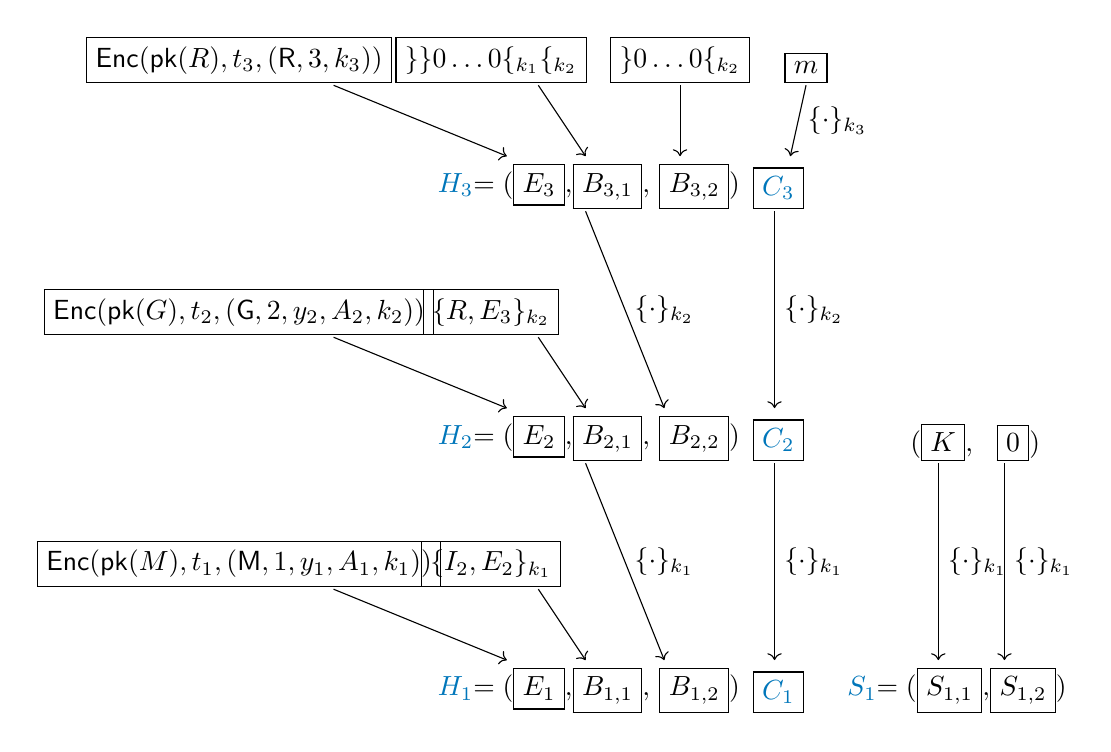
\begin{tikzpicture}[scale=0.4]

\def\x{-4} 

\def\a{0} 

\def\b{0}

% O3

\draw (0,\x+\a) node [above right] {\textcolor{hybrid}{$H_3$}$ = ($\fbox{$E_3$}$, $\fbox{$B_{3,1}$}$,$ \fbox{$B_{3,2}$}$)$};

\draw (8,\a) node [above] {\fbox{$\}0\dots0\{_{k_2}$}}; 
\draw[->] (8,\a+0.25) -- (8,\a+\x/2+.0);

\draw (2,\a) node [above] {\fbox{$\}\}0\dots0\{_{k_1}\{_{k_2}$}};
\draw[->] (3.5,\a+0.25) -- (5,\a+\x/2+.0);

\draw (-6,\a) node [above]{\fbox{$\enc(\pk(R),t_3,(\mathsf{R}, 3, k_3))$}};
\draw[->] (-3,\a+0.25) -- (2.5,\a+\x/2+.0);

\draw (10,\x+\a) node [above right] {\fbox{\textcolor{hybrid}{$C_3$}}}; 
\draw (12,\a) node [above] {\fbox{$m$}}; 
\draw[->] (12,\a+0.25) -- node[anchor=west]{$\{\cdot\}_{k_3}$}(11.5,\a+\x/2+.0);

% O2

\draw (2,\a+2*\x) node [above] {\fbox{$\{R,E_3\}_{k_2}$}};

\draw (-6,\a+2*\x) node [above]{\fbox{$\enc(\pk(G),t_2,(\mathsf{G}, 2, y_2, A_2, k_2))$}};

\draw (0,\a+3*\x) node [above right] {\textcolor{hybrid}{$H_2$}$ = ($\fbox{$E_2$}$, $\fbox{$B_{2,1}$}$,$ \fbox{$B_{2,2}$}$)$}; 

\draw[->] (5,\a+1*\x+.25) -- node[anchor=west]{$\{\cdot\}_{k_2}$} (7.5,\a+2.5*\x+.0);

\draw[->] (3.5,\a+2*\x+.25) -- (5,\a+2.5*\x+.0);

\draw[->] (-3,\a+2*\x+.25) -- (2.5,\a+2.5*\x+.0); 

\draw (10,\a+3*\x) node [above right] {\fbox{\textcolor{hybrid}{$C_2$}}}; 
\draw[->] (11,\a+1*\x+.25) -- node[anchor=west]{$\{\cdot\}_{k_2}$} (11,\a+2.5*\x+.0);

\draw (15,\a+3*\x) node [above right] {$($\fbox{$K$}$, \hspace{3mm} $\fbox{$0$}$)$};

% O1

\draw (2,\a+4*\x) node [above] {\fbox{$\{I_2,E_2\}_{k_1}$}};

\draw (-6,\a+4*\x) node [above]{\fbox{$\enc(\pk(M),t_1,(\mathsf{M}, 1, y_1, A_1, k_1))$}};

\draw (0,\a+5*\x) node [above right] {\textcolor{hybrid}{$H_1$}$ = ($\fbox{$E_1$}$, $\fbox{$B_{1,1}$}$,$ \fbox{$B_{1,2}$}$)$}; 

\draw[->] (5,\a+3*\x+0.25) -- node[anchor=west]{$\{\cdot\}_{k_1}$} (7.5,\a+4.5*\x+.0); 

\draw[->] (3.5,\a+4*\x+.25) -- (5,\a+4.5*\x+.0);

\draw[->] (-3,\a+4*\x+.25) -- (2.5,\a+4.5*\x+.0);

\draw (10,\a+5*\x) node [above right] {\fbox{\textcolor{hybrid}{$C_1$}}}; 
\draw[->] (11,\a+3*\x+.25) -- node[anchor=west]{$\{\cdot\}_{k_1}$} (11,\a+4.5*\x+.0);

\draw (13,\a+5*\x) node [above right] {\textcolor{hybrid}{$S_1$}$ = ($\fbox{$S_{1, 1}$}$, $\fbox{$S_{1,2}$}$)$};

\draw[->] (16.2,\a+3*\x+.25) -- node[anchor=west]{$\{\cdot\}_{k_1}$} (16.2,\a+4.5*\x+.0);

\draw[->] (18.3,\a+3*\x+.25) -- node[anchor=west]{$\{\cdot\}_{k_1}$} (18.3,\a+4.5*\x+.0);

\end{tikzpicture}
\endgroup
}
\fi
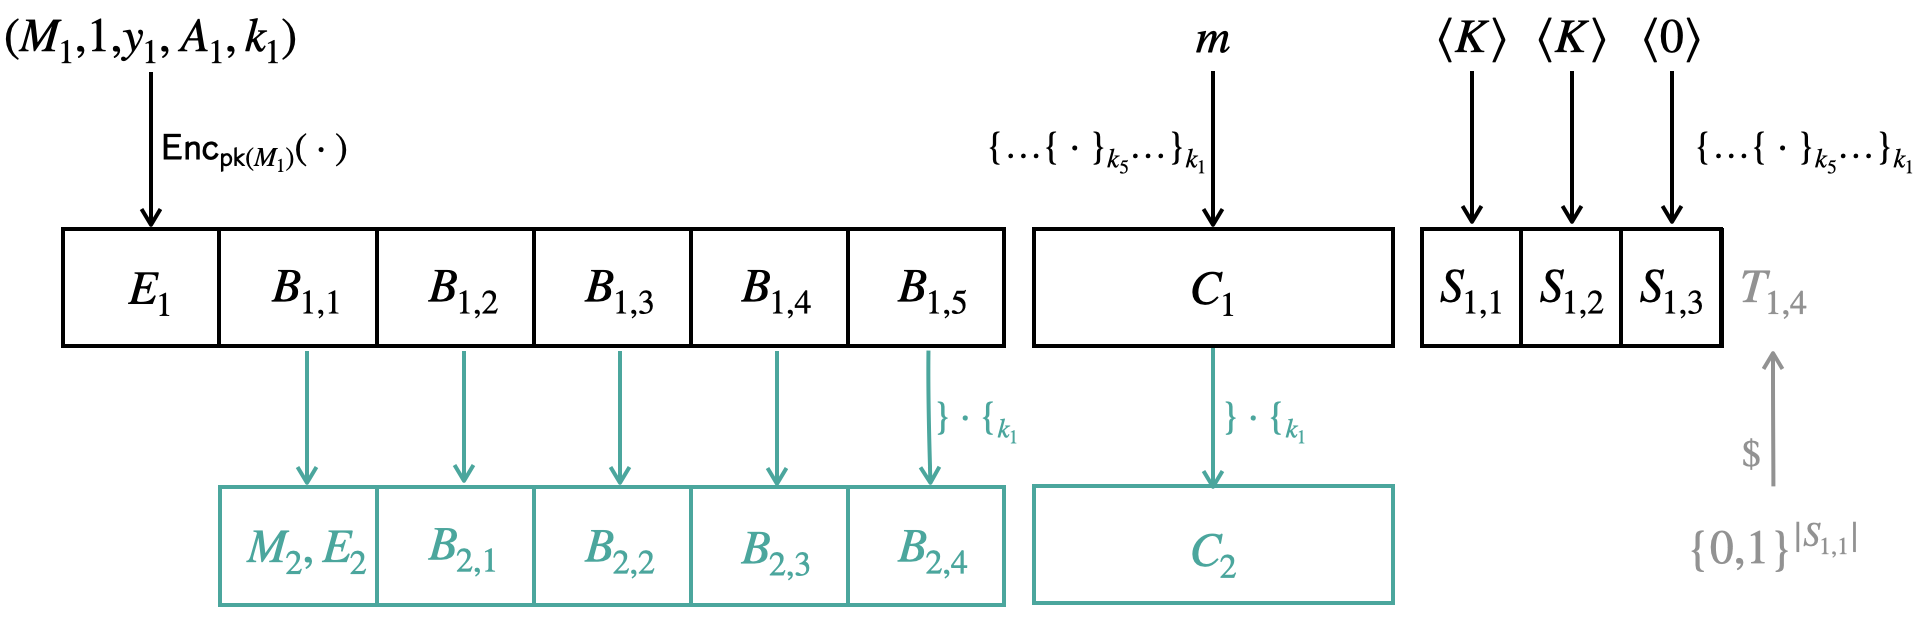
\includegraphics[width=0.8\textwidth]{template/onion2.png}
\caption{\footnotesize{\textcolor{black}{A pictorial description of how an onion is formed using TOES. The verification hashes $A_1$ for $M_1$ are the hashes $h(S_{1,1}, S_{1,2}, S_{1,3})$, $h(S_{1,2}, S_{1,3}, T_{1,4})$, $h(S_{1,3}, T_{1,4}, S_{1,1})$, and $h(T_{1,4}, S_{1,1}, S_{1,2})$ in lexicographical order, where $T_{1,4} \sample \bin^{|S_{1,1}|}$. }
}
}
\label{fig:formonion}
\end{figure}

\paragraph{Forming an onion with an incomplete path.}
We form an onion for a path that begins and/or ends with the empty path, e.g., $(\bot, \bot, P_3, P_4, P_5, \bot, \dots, \bot)$, by setting the intermediary party for the empty locations (the $\bot$'s) to be the sender; and if the recipient is $\bot$, the sepal blocks are all dummy sepal blocks $\langle 0 \rangle$. In this case, the algorithm outputs only the onion vectors for the parties corresponding to non-empty locations on the path.

\paragraph{Remark on the onion size.}
Recall that $\ell_1$ is the number of mixers on a routing path, and $\ell_2$ is the number of gatekeepers. 
Each onion consists of a content block, a number of sepal blocks, and a number of header blocks. The length of each message block is just the length of a message (let us call this $\ell_m$). Each onion layer consists of at most $\ell_1+1$ sepal blocks and $\ell_1 + \ell_2 + 1$ header blocks, where the length of each sepal block is the length of each layer key (so, roughly $\secpar$), and the length of each header block is dominated by the size of the verification hashes in a layer (so, roughly $\bigO{\secpar \ell_1}$). Thus, the overall size of a tulip bulb is $\bigO{\secpar(\ell_1^2+\ell_2)} + \ell_m$. 

%Recall that $\ell$ is the length of the routing path, and $\ell_1$ is the number of mixers on the path. A tulip bulb consists of the header blocks (one $E$-block and $\ell-2$ $B$-blocks), the $\ell_1+1$ sepal blocks, and content block. The content block size and the sepal block size are independent of $\ell$ and determined by the message length and the layer key length, respectively. The header block size depends on $\ell_1$: each block contains the $\ell_1+2$ verification hash values in addition to the role, the index, the nonce, and the layer key. Thus, the size of the tulip bulb is $\bigO{\ell^2 \cdot \mathsf{keyLen} + \mathsf{messageLen}}$, where $\mathsf{messageLen}$ is the size of a message, and $\mathsf{keyLen}$ is the size of a key for a block cipher (roughly the same as the security parameter).



\subsection{Proof of security} \label{sec:securityproof}
\newcommand{\hybrid}[1]{\mathsf{Hybrid}_{#1}} 

Here, we summarize our proof that our construction satisfies the definition of security provided in Definition~\ref{def:secure}.

\begin{theorem} \label{thm:security} 
Tulip Onion Encryption Scheme is bruisable-onion secure, assuming the  existence of CCA2-secure public key encryption schemes with tags, 
block ciphers, and 
collision-resistant hash functions.
\end{theorem}

\begin{proof}[Proof idea]
We first provide a hybrid argument for the case where the challenge onion is too bruised to recover the innermost onion. Proofs for the other cases (when the onion is recoverable and/or when the recipient is honest) are given after the proof of this first case. % we provide in full here. \todo{edit this if more cases are added}

Below, we describe a sequence of hybrid experiments $\hybrid{0}, \dots, \hybrid{18}$ and provide a brief explanation ({\color{hybrid} in color}) of why each pair of consecutive experiments consists of indistinguishable scenarios. (More details on the proofs of indistinguishability can be founds in Appendix~\ref{app:security}.)
Recall that in the security game $\mathsf{BrOnSHH}$, the honest mixer is $M_{i_1}$, sitting in position $1 \le i_1 \le l_1$; and the honest gatekeeper is $G_{j=i_2-\ell_1}$, sitting in position $\ell_1+1 \le i_2 \le \ell_2$. %; and the honest recipient is $R$.


%%% OUTERMOST 
\medskip
\noindent $\hybrid{0}$: the challenge onion $O_1$ is formed correctly. (This is the same as the game when $b=0$.)  

    \textcolor{hybrid}{$\updownarrow$ Indistinguishable from CCA2-secure public key encryption.}

\noindent $\hybrid{1}$: same as $\hybrid{0}$ except that the ciphertext $E_{i_1}$ is an encryption under $\pk(M_{i_1})$ of the dummy key $0$. (The challenger still samples for the layer key $k_{i_1}$ and uses it to form the $i_1^\mathit{th}$ onion layers $\vec{O}_{i_1}$.) 

    \textcolor{hybrid}{$\updownarrow$ Indistinguishable from the collision resistance of the hash function}

\noindent $\hybrid{2}$: same as $\hybrid{1}$ except that if, in the second query phase, the challenger receives an onion $O = ((E, B), C, S) \not\in \vec{O}_{i_1}$ such that $E=E_{i_1}$, the challenger responds with $\bot$ (rather than processing $O$). 

    \textcolor{hybrid}{$\updownarrow$ Indistinguishable from PRP security.}

\noindent $\hybrid{3}$: same as $\hybrid{2}$ except that the challenger forms the $i_1^\mathit{th}$ onion layers $\vec{O}_{i_1}$ using a truly random permutation rather than a PRP keyed with $k_{i_1}$. 

    \textcolor{hybrid}{$\updownarrow$ Identically distributed since $\vec{O}_{i_1-1}, \dots, \vec{O}_1$ are wrapped around truly random blocks.}

\noindent $\hybrid{4}$: same as $\hybrid{3}$ except that the challenger uses the dummy message content $\bot$ and the truncated path $(M_1, \dots, M_{i_1}, \vec{\bot})$ and associated sequence $(y_1, \dots, y_{i_1}, \vec{\bot})$ of metadata (instead of the real message and full path and sequence of metadata) to form $O_1$.

    \textcolor{hybrid}{$\updownarrow$ Identically distributed since the inner layers $\vec{O}_\ell, \dots, \vec{O}_{i_1+1}$ are independent of the path up to $M_{i_1}$.} 

\noindent $\hybrid{5}$: same as $\hybrid{4}$ except that the first query to peel or bruise an onion $O_{i_1} = O_{i_1, k} \in \vec{O}_{i_1}$ on behalf of $M_{i_1}$ peels to a new onion formed using the message $m$, the routing path $(\vec{\bot}, M_{i_1+1}, \dots, R)$, and the associated sequence of metadata $(\vec{\bot}, y_{i_1+1}, \dots, y_{\ell-1})$. (The newly formed onion $O_{i_1+1}$ has the correct number $k$ of bruises.)

    \textcolor{hybrid}{$\updownarrow$ Indistinguishable from PRP security.}

\noindent $\hybrid{6}$: same as $\hybrid{5}$ except that the challenger forms the $i_1^\mathit{th}$ onion layers $\vec{O}_{i_1}$ using the PRP keyed with $k_{i_1}$ instead of a truly random permutation. 

    \textcolor{hybrid}{$\updownarrow$ Indistinguishable from CCA2-security.}

\noindent $\hybrid{7}$: same as $\hybrid{6}$ except that the ciphertext $E_{i_1}$ is an encryption of the real key $k_{i_1}$ rather than the dummy key $0$. (At this stage, the challenge onion $O_1$ is same as that in the game when $b=1$, but the onions returned by $M_{i_1}$ and $G_j$ are not quite the same as when $b=1$. The challenger forms $O_1$ using the message $\bot$, the routing path $(M_1, \dots, M_{i_1}, \vec{\bot})$, and the metadata $(y_1, \dots, y_{i_1}, \vec{\bot})$. The onion $O_{i_1+1}$ returned by the challenger on behalf of the mixer $M_{i_1}$ is a new onion with the correct number of bruises, formed by running $\formonion$ on $m$, $(\vec{\bot}, M_{i_1+1}, \dots, R)$, and the metadata $(\vec{\bot}, y_{i_1+1}, \dots, y_{\ell-1})$. The challenger obtains the onion $O_{i_2+1}$ returned by the on behalf of the gatekeeper $G_{j}$ by running $\proconion$ on the query onion.)

%%% MIDDLE LAYERS
    \textcolor{hybrid}{$\updownarrow$ Indistinguishable from CCA2-secure public key encryption.}

\noindent $\hybrid{8}$: same as $\hybrid{7}$ except that the ciphertext $E_{i_2}$ is an encryption under $\pk(G_{j})$ of the dummy key $0$. (The challenger still samples for the layer key $k_{i_2}$ and uses it to form the $i_2^\mathit{th}$ onion layers $\vec{O}_{i_2}$.) 

    \textcolor{hybrid}{$\updownarrow$ Indistinguishable from the collision resistance of the hash function}

\noindent $\hybrid{9}$: same as $\hybrid{8}$ except that if, in the second query phase, the challenger receives an onion $O = ((E, B), C, S) \not\in \vec{O}_{i_2}$ such that $E=E_{i_2}$, the challenger responds with $\bot$ (rather than processing $O$). 

    \textcolor{hybrid}{$\updownarrow$ Indistinguishable from PRP security.}

\noindent $\hybrid{10}$: same as $\hybrid{9}$ except that the challenger forms the $i_2^\mathit{th}$ onion layers $\vec{O}_{i_2}$ using a truly random permutation rather than a PRP keyed with $k_{i_2}$. 

    \textcolor{hybrid}{$\updownarrow$ Identically distributed since $\vec{O}_{i_2-1}, \dots, \vec{O}_{i_1+1}$ are wrapped around truly random blocks.}

\noindent $\hybrid{11}$: same as $\hybrid{10}$ except that the challenger uses the path $(\vec{\bot}, M_{i_1+1}, \dots,$ $G_{j}, \vec{\bot})$ and associated sequence of metadata (instead of the real message and full path and sequence of metadata) to form $O_{i_1+1}$.

    \textcolor{hybrid}{$\updownarrow$ Identically distributed since the inner layers $\vec{O}_\ell, \dots, \vec{O}_{i_2+1}$ are independent of the path up to $G_j$.} 

\noindent $\hybrid{12}$: same as $\hybrid{11}$ except that the first query to peel or bruise an onion $O_{i_2} = O_{i_2, k} \in \vec{O}_{i_2}$ on behalf of $G_j$ peels to a new onion formed using the message $m$, the routing path $(\vec{\bot}, G_{j+1}, \dots, R)$, and the associated sequence of metadata. (The newly formed onion $O_{i_2+1}$ has the correct number $k$ of bruises.)

    \textcolor{hybrid}{$\updownarrow$ Indistinguishable from PRP security.}

\noindent $\hybrid{13}$: same as $\hybrid{12}$ except that the challenger forms the $i_2^\mathit{th}$ onion layers $\vec{O}_{i_2}$ using the PRP keyed with $k_{i_2}$ instead of a truly random permutation. 

    \textcolor{hybrid}{$\updownarrow$ Indistinguishable from CCA2-security.}

\noindent $\hybrid{14}$: same as $\hybrid{13}$ except that the ciphertext $E_{i_2}$ is an encryption of the real key $k_{i_2}$ rather than the dummy key $0$. 

    \textcolor{hybrid}{$\updownarrow$ Identically distributed since the sepals are truly random blocks wrapped in layers on encryption, and the verification hashes don't reveal how bruised the sepals are.}

\noindent $\hybrid{15}$: same as $\hybrid{14}$ except for how bruised the onion $O_{i_1+1}$ is.  The onion $O_{i_1+1}$ that $M_{i_1}$ returns will be completely unbruised.  The challenger remembers how bruised $O_{i_1}$ was, however, and forms the the onion $O_{i_2+1}$ accordingly; thus, $O_{i_2+1}$ is formed identically as in $\hybrid{11}$. 
(At this stage, the challenge onions $O_1$ and $O_{i_1+1}$ are the same as that in the game when $b=1$, but the onion returned by $G_j$ is not quite the same as when $b=1$.)

%%%% INNERMOST 

    \textcolor{hybrid}{$\updownarrow$ Indistinguishable from PRP security.}

\noindent $\hybrid{16}$: same as $\hybrid{15}$ except that the challenger forms the penultimate onion layers $\vec{O}_{\ell-1}$ using a truly random permutation rather than a PRP keyed with $k_{\ell-1}$. 

    \textcolor{hybrid}{$\updownarrow$ Identically distributed because since $\vec{O}_{\ell-2}, \dots, \vec{O}_{i_2+1}$ are wrapped truly random blocks.}

\noindent $\hybrid{17}$: same as $\hybrid{16}$ except that the challenger uses the message $\bot$ and the recipient $\bot$. 

    \textcolor{hybrid}{$\updownarrow$ Indistinguishable from PRP security.}

\noindent $\hybrid{18}$: same as $\hybrid{17}$ except that the challenger forms the penultimate onion layers $\vec{O}_{\ell-1}$ using the PRP keyed with $k_{\ell-1}$ instead of a truly random permutation. Note that $\hybrid{18}$ is indistinguishable to the case when $b=1$.

The hybrid argument for the case where the challenge onion is recoverable, and the recipient is honest is the same as above, except that, in $\hybrid{17}$, only the message is $\bot$ (the recipient remains $R$). 
When the recipient is adversarial, the hybrid argument is just $\hybrid{0}$-$\hybrid{15}$ above (without $\hybrid{16}$-$\hybrid{18}$). 
%\todo{Hybrid arguments for other cases}
%
\iffalse 
    \textcolor{hybrid}{$\updownarrow$ Indistinguishable from CCA2-security.}

\noindent $\hybrid{9}$: same as $\hybrid{8}$ except that that the ciphertext $E_{i_2}$ is an encryption under $\pk(G_{j})$ of the dummy key $0$. (The challenger still samples for the layer key $k_{i_2}$ and uses it to form the $i_2^\mathit{th}$ onion layers $\vec{O}_{i_2}$.)

    \textcolor{hybrid}{$\updownarrow$ Indistinguishable from the collision resistance of the hash function}

\noindent $\hybrid{10}$: same as $\hybrid{9}$ except that if, in the second query phase, the challenger receives an onion $O = ((E, B), C, S) \not\in \vec{O}_{i_2}$ such that $E=E_{i_2}$, the challenger responds with $\bot$ (rather than processing $O$). 

    \textcolor{hybrid}{$\updownarrow$ Indistinguishable from PRP security.}

\noindent $\hybrid{11}$: same as $\hybrid{10}$ except that the the challenger forms the $i_2^\mathit{th}$ onion layers $\vec{O}_{i_2}$ using a truly random permutation rather than a PRP keyed with $k_{i_2}$.\todo{Edited up to here.}

    \textcolor{hybrid}{$\updownarrow$ Identically distributed since $\vec{O}_{i_2}, \dots, \vec{O}_{i+1}$ are wrapped around truly random blocks.}

\noindent $\hybrid{12}$: same as $\hybrid{11}$ except that rather than ``processing'' $O_{i_2}$ (inverting the random permutation) to get the onion $O_{i_2+1}$, the challenger forms a new onion with the correct remaining routing path $(\vec{\bot}, G_{j+1}, \dots, R)$ and sequence of metadata $(\vec{\bot}, y_{i_2+1}, \dots, y_{\ell-1})$ (and message $m$). %message (and $\bot$ for all the participants on the routing path preceding $G_{i_2}$).  
This results in $\ell_1+1$ candidates for $O_{i_2+1}$; the challenger picks the one that corresponds to the same number of bruises as $O_{i_2}$.
%
%    \textcolor{hybrid}{$\updownarrow$ Identically distributed by construction.}
%
%\noindent $\hybrid{10}$: same as $\hybrid{9}$ except that we explicitly note:  
In the event that $O_{i_2}$ was already bruised more than $\theta\ell_1$ times, in the onion $O_{i_2+1}$, 
the sepal content is the dummy key $0$ (i.e., the master key $K$ is not recoverable from $O_{i_2+1}$); otherwise if $O_{i_2}$ is not too bruised, the sepal contains $K$ (i.e., the key is recoverable). 

    \textcolor{hybrid}{$\updownarrow$ Indistinguishable from PRP security.}

\noindent $\hybrid{13}$: same as $\hybrid{12}$ except that, in the event that the onion is too bruised, %the last header block $B_{i_2+1, \ell-i_2+1}$\todo{Check this!} is an encryption containing the empty recipient $\bot$ (as opposed to $R$), and the message content is also $\bot$ (as opposed to $m$).  
to get the onion $O_{i_2+1}$, the challenger forms a new onion with the correct remaining gatekeepers but not the recipient $(\vec{\bot}, G_{j+1}, \dots, G_{\ell_2}, \bot)$, the sequence of metadata $(\vec{\bot}, y_{i_2+1}, \dots, y_{\ell-1})$, and the empty message $\bot$.
%If the onion is not too bruised, then $O_{i_2+1}$ is (same as in $\hybrid{9}$) formed as a brand new onion with the master key $K$ and correct layer keys for the remaining gatekeepers and recipient.  
This way, (1) the original challenge onion $O_1$ is distributed as when $b=1$; (2) the onion $O_{i_2+1}$ returned by $G_{i_2}$ is distributed the same way as when $b=1$ in the event that the recipient is controlled by the adversary.  The onion $O_{i_1+1}$ returned by $M_{i_1}$ is still not exactly as in the $b=1$ case, which we will address in the next few hybrids.

    \textcolor{hybrid}{$\updownarrow$ Identically distributed because the onion layer for $G_{j}$ is formed using a truly random permutation instead of one keyed by $k_{i_2}$, see $\hybrid{11}$.
    }

\noindent $\hybrid{14}$: same as $\hybrid{13}$ except in how the onion $O_{i_1+1}$ is formed.  It will be formed with the routing path that ends in $G_{i_2}$, and contains $\bot$ for all the gatekeepers following $G_{i_2}$, and $(\bot,\bot)$ for the recipient and message (but the layer for $G_{i_2}$ is still formed using a truly random permutation). Then let $O_{i_1+1}$ be the onion that corresponds to the correct amount of bruising, i.e., if the adversary's query to $M_{i_1}$ was to peel $O_{i_1,k}$, then $O_{i_1+1}$ is the onion that has been bruised $k$ times. 

    \textcolor{hybrid}{$\updownarrow$ Identically distributed because the onion layer for $G_{i_2}$ is formed using a truly random permutation instead of one keyed by $k_{i_2}$, see $\hybrid{11}$.
    }

\noindent $\hybrid{15}$: same as $\hybrid{14}$ except for how bruised the onion $O_{i_1+1}$ is.  The onion $O_{i_1+1}$ that $M_{i_1}$ returns will be completely unbruised.  The challenger remembers how bruised $O_{i_1}$ was, however, and forms the the onion $O_{i_2+1}$ accordingly; thus, $O_{i_2+1}$ is formed identically as in $\hybrid{11}$.  Now, $O_{i_1+1}$ is almost as in the case when $b=1$  except that the layer key $k_{i_2}$ does not exist, and $E_{i_2}$ is an encryption of $0$; instead, a truly random permutation is used for layer $O_{i_2}$. 

    \textcolor{hybrid}{$\updownarrow$ Indistinguishable from PRP security.}

\noindent $\hybrid{16}$: same as $\hybrid{15}$ except that the challenger forms the $i_2^\mathit{th}$ layer using the PRP keyed with $k_{i_2}$ instead of a truly random permutation. ($E_{i_2}$ is still an encryption of $0$ rather than $k_{i_2}$.) 

    \textcolor{hybrid}{$\updownarrow$ Indistinguishable from CCA2-security.}

\noindent $\hybrid{17}$: same as $\hybrid{16}$ except that, when forming $O_{i_1+1}$, the ciphertext $E_{i_2}$ is an encryption of the real key $k_{i_2}$, rather than the dummy key $0$.  Now, (1) the original challenge onion $O_1$ is distributed as when $b=1$; (2) the onion $O_{i_1+1}$ returned by the honest mixer $M_{i_1}$ is distributed as when $b=1$; and n the event that the recipient is controlled by the adversary, (3) the onion $O_{i_2+1}$ returned by $G_{j}$ is distributed as when $b=1$. (The remaining hybrid will address the case when the recipient is honest.)

\textcolor{hybrid}{$\updownarrow$ Indistinguishable by CCA-security of the recipient's encryption scheme.}\todo{Check this!}

\noindent $\hybrid{18}$: same as $\hybrid{17}$ except that, in the event that the recipient is honest, when forming $O_{i_2+1}$, the challenger always sets $m=\bot$.  Note that $\hybrid{16}$ is identical to the case when $b=1$.
\fi
\end{proof}

\newcommand{\protocol}{\Pi_t}
\section{Our Onion Routing Protocol, $\protocol$} \label{sec:dp} 

\iffalse 
\paragraph{In a nutshell:} The input to each party~$P_i$ is a singleton $\sigma_i = \{(m_i, R_i)\}$ consisting of a message~$m_i$ and a recipient~$R_i$; the idea being that $P_i$ should send the message~$m_i$ to the recipient~$R_i$. First, $P_i$ forms an onion bearing $m_i$ for $R_i$. $P_i$ also forms a few (polylog in the security parameter number) of checkpoint dummy onions, each bearing the empty message $\bot$ for a randomly selected recipient. 
We provide the exact algorithms that $P_i$ follows as the sender in Section~\ref{sec:formonions}. 

After forming the onions, $P_i$ sends them out in random order, each to the first intermediary party on its routing path. 
At this point, $P_i$ acts as an intermediary/recipient waiting to receive onions that other parties formed. 
We provide the algorithm that $P_i$ follows as an intermediary/recipient in Section~\ref{sec:proconions}. 
\fi

\subsection{Choosing the onion parameters} \label{sec:formonions}

We describe our anonymous onion routing protocol, $\protocol$. %\todo{For checkpoint onions, use the metadata to communicate with the intermediaries}

Let $\mathsf{TOES}=(\keygen, \formonion, \proconion, \proconionhelper, \bruiseonion)$ be the bruisable onion encryption scheme in Section~\ref{sec:boes}. 
Let $\ell_1$ be the number of mixers on the routing path, 
let $\ell_2$ be the number of gatekeepers, and 
let $\ell_3$ be the (expected) number of onions at each intermediary per hop. 
Let $F_1$ and $F_2$ be pseudorandom functions (PRFs) such that $F_1$ outputs zero with frequency $(\ell_1+\ell_2)\ell_3/|\parties| = (\ell_1+\ell_2)\ell_3/N = \bigOmega{\polylog\thinspace\secpar}/N$, and the range of $F_2$ is superpolynomial in the security parameter~$\secpar$. 
We assume a setup with a public key infrastructure (PKI); note that the PKI enables each pair of parties $(P_i, P_k)$ to set up a shared secret key $\sk_{i, k}$,e.g., by using Diffie-Hellman key exchange. 

For each sender $P_i$, let $\sigma_i$ denote the input for $P_i$. 
For each $(m_i, R_i)\in\sigma_i$, party $P_i$ forms an onion bearing the message $m_i$ to the recipient $R_i$. Additionally, $P_i$ forms a polylog (in the security parameter) number of checkpoint onions. 

The algorithms for forming the onions are essentially those of $\Pi_a$~\cite{ICALP:AndLysUpf18}, except we use tulip bulbs instead of standard ones. 
Specifically, we use tulip bulbs with $\ell_1 = \bigOmega{\polylog\thinspace\secpar}$ mixers per onion, $\ell_2 = \bigOmega{\polylog\thinspace\secpar}$ gatekeepers per onion, and $d = \theta\ell_1$ key-blocks per sepal. %Note that in prior sections, we denoted the number of mixers by $\ell$, and we are changing the notation here; (here, $\ell_1$ is $\ell$). 
For completeness, we describe these algorithms in detail below. 

\paragraph{Forming the message-bearing onions.}
To form the message-bearing onion for the message-recipient pair $(m_i, R_i) \in \sigma_i$, $P_i$ first samples $\ell_1+ \ell_2$ parties $M_1, \dots, M_{\ell_1}$, $G_1, \dots, G_{\ell_2}$ uniformly at random and then runs the onion-forming algorithm $\formonion$ on  
    the message $m_i$, 
    the routing path $\vec{P} = (M_1, \dots, M_{\ell_1}, G_1, \dots, G_{\ell_2},$ $ R_i)$, 
    the public keys associated with the parties in $\vec{P}$ (which we will denote $\pk(\vec{P})$), and 
    the sequence $\vec{\bot}= (\overbrace{\bot, \bot, \dots, \bot}^{\ell_1 + \ell_2 \text{ times}})$ of metadata.
Here, ``$\bot$'' denotes the empty metadata. %See Figure~\ref{fig:mbo} below for the pseudocode. 

\iffalse
\begin{figure} [ht!]
\begin{pchstack} [center, boxed]
\pseudocode[linenumbering]{
M_1, \dots, M_{\ell_1}, G_1, \dots, G_{\ell_2} \sample \parties \\
\vec{\bot} = (\overbrace{\bot, \bot, \dots, \bot}^{\ell_1 + \ell_2\text{ times}}) \\
\vec{O} \gets \formonion(m, (M_1, \dots, M_{\ell_1}, G_1, \dots, G_{\ell_2}, R_i), \pk(\vec{P}), \vec{\bot})
}
\end{pchstack}
\caption{\footnotesize{Pseudocode for forming the message-bearing onion}}
\label{fig:mbo}
\end{figure}
\fi

\paragraph{Forming the checkpoint onions.} 
Next, $P_i$ forms the checkpoint onions. 
$P_i$ initializes the sets of nonces, $\mathcal{Y}_1, \dots, \mathcal{Y}_{\ell_1}$, to the empty set. 

Then, for every pair $(j, P_k)$ where $j \in [\ell_1]$ is a hop-index and $P_k\in\parties$ is a party, $P_i$ determines whether or not they should form an onion for party $P_k$ to be verified in the $j^{th}$ hop. 
This is done by computing the pseudorandom function $F_1$ on the shared key $\sk_{i, k}$ and the hop-index $j$. 
If the output equals zero, $P_i$ 
sets the checkpoint nonce $y$ to $ F_2(\sk_{i, k}, j)$; 
adds $y$ to the nonce-set $\mathcal{Y}_j$; 
samples $\ell_1+ \ell_2+1$ parties $M_{1}, \dots, M_{\ell_1}, G_{1}, \dots, G_{\ell_2}, R$ uniformly at random; and 
forms a checkpoint onion by running $\formonion$ on 
    the empty message ``$\bot$,'' 
    the routing path $\vec{P} = (M_{1}, \dots, M_{\ell_1}, G_{1}, \dots, G_{\ell_2}, R)$, 
    the public keys $\pk(\vec{P})$ associated with the parties on the path, and 
    the sequence $\vec{y} =(\overbrace{\bot, \bot, \dots, \bot}^{j-1 \text{ times}}, y, \overbrace{\bot, \bot, \dots, \bot}^{\ell_1+\ell_2-j \text{ times}})$ of metadata.
%See Figure~\ref{fig:cpo} below for the pseudocode. 
\iffalse
\begin{figure} [ht!]
\begin{pchstack} [center, boxed]
\pseudocode[linenumbering]{
\mathcal{Y}_1, \dots, \mathcal{Y}_{\ell_1} \gets \emptyset \\
\pcfor (j, P_k) \in [\ell_1] \times \parties: \\
\pcind \pcif F_1(\sk_{i, k}, j) = 0: \\
\pcind \pcind y \gets F_2(\sk_{i, k}, j) \\
\pcind \pcind \mathcal{Y}_j \gets \mathcal{Y}_j.\mathsf{append}(y) \\
\pcind \pcind \vec{y} = (\overbrace{\bot, \bot, \dots, \bot}^{j-1 \text{ times}}, y, \overbrace{\bot, \bot, \dots, \bot}^{\ell_1+\ell_2-j \text{ times}}) \\
\pcind \pcind M_{1}, \dots, M_{\ell_1}, G_{1}, \dots, G_{\ell_2}, R \sample \parties \\
\pcind \pcind \vec{O} \gets \formonion(\bot, (M_{1}, \dots, M_{\ell_1}, G_{1}, \dots, G_{\ell_2}, R), \pk(\vec{P}), \vec{y})  
}
\end{pchstack}
    \caption{\footnotesize{Pseudocode for forming checkpoint onions}}
    \label{fig:cpo}
\end{figure}
\fi

\subsection{Routing onions} \label{sec:proconions} 
After forming the onions, $P_i$ releases them into the network. From this point on, $P_i$ acts as an intermediary or recipient. 
That is, $P_i$ first sends each of its onions to the first party on the onion's routing path and then waits to receive onions. 
In contrast to the setup for $\Pi_a$, here, the honest parties must determine when to send out batch-processed onions without relying on a global clock; accordingly, our protocol for processing and routing tulip bulbs (i.e., onions) differs from that of $\Pi_a$.

To begin with, $P_i$ sets counters $c_1, \dots, c_{\ell_1}, j$ to zero. 

Upon receiving an onion $O$, $P_i$ processes it: That is, $P_i$ first peels the onion. $P_i$ drops the onion if this produces a layer key that $P_i$ has seen before; that is, the layer key also serves as a session id for preventing replay attacks. 
What happens next depends on $P_i$'s role:
\begin{itemize}
\item ($\mathbf{Role} = \mathsf{Recipient}$) If the peeled onion $O'$ is a message for $P_i$, $P_i$ outputs it.  

\item ($\mathbf{Role} = \mathsf{Gatekeeper}$) If $P_i$ is a gatekeeper for $O$ and peeling $O$ produces a peeled onion $O'$ and a destination $P'$ for $O'$, $P_i$ sends $O'$ to $P'$ right away. (Note that if $P_i$ is the last gatekeeper on the routing path, $P_i$ can recover the identity of the recipient $R$ and the onion for $R$ only if a sufficiently small number of mixers bruised the onion en route. See Section~\ref{sec:boes} to recall how the onion encryption construction works and its security properties.)  

\item ($\mathbf{Role} = \mathsf{Mixer}$)  Otherwise if $P_i$ is a mixer for $O$, $P_i$ determines whether $O$ was received ``on time'' or not (relative to $P_i$'s internal clock). 
%If $P_i$ is a regular intermediary (i.e., $P_i = I_j$ for some $j \le \ell_1-1$) and and 
If $O$ arrived late, $P_i$ bruises the onion $O$ and immediately sends the bruised onion $O''$ to its next destination. If $P_i$ is the last mixer on the routing path (i.e., $P_i = M_{\ell_1}$), $P_i$ sends the peeled onion $O'$ to the first gatekeeper $G_1$. 

\hspace{4mm} Otherwise if $O$ is either early or on time, $P_i$ places the peeled onion $O'$  (along with its next destination $P'$) in its message outbox. 
If processing $O$ reveals the non-empty nonce $y \neq \bot$, then $P_{i}$ first checks whether $y$ belongs in a set $\mathcal{Y}_k$. (Recall from Section~\ref{sec:formonions} that $\mathcal{Y}_k$ is the set of $k^{th}$ layer checkpoint nonces $P_i$ expects to see from the onions it receives.) If it does, then $P_i$ increments $c_k$ by one, and %i.e., $c_k \gets c_k+1$; and 
updates $\mathcal{Y}_k$ to exclude $y$. 

\hspace{4mm} Upon processing sufficiently many $j^{th}$ layer onions (i.e., if $c_j \ge \tau|\mathcal{Y}_j|$ where $0 < \tau \le 1$ is a system parameter), $P_i$ %resets $c$ to zero, 
sends out these onions (but not the onions for future hops) in random order, and advances its local clock (i.e., increments $j$ by one). %, i.e., $j \gets j+1$). 
Note that onions are shuffled at honest intermediaries when they are batch-processed and sent out in random order. 
%See Figure~\ref{fig:proconions} for the pseudocode.
\end{itemize} 

\iffalse
\begin{figure}[ht!]
\begin{pchstack} [center, boxed]
\pseudocode[linenumbering]{
c_1, \dots, c_{\ell_1}, j \gets 0 \\
\textbf{upon receiving $O$} \\
\pcind (\mathsf{Role}, k, y, O', P') \gets \proconion(\sk(P_i), O) \\
\pcind \pcif \mathsf{Role} = \mathsf{Recipient} \\
\pcind \pcind \pcreturn O' \\
\pcind \pcif k < j \\
\pcind \pcind \pcif \mathsf{Role} = \mathsf{Gatekeeper} \\
\pcind \pcind \pcind \textbf{send $O'$ to $P'$} \\
\pcind \pcind \pcelse \pccomment{$\mathsf{Role} = \mathsf{Mixer}$} \\
\pcind \pcind \pcind O'' \gets \bruiseonion(\sk(P_i), O) \\
\pcind \pcind \pcind \textbf{send $O''$ to $P'$} \\
\pcind \pcelse \pccomment{$k \ge j$} \\
\pcind \pcind \textbf{place $(O', P')$ in outbox} \\
\pcind \pcind \pcif (y \neq \bot) \land (\exists k \textbf{ s.t.~$y \in \mathcal{Y}_k$)} \\
\pcind \pcind \pcind \mathcal{Y}_k \gets \mathcal{Y}_k\setminus\{y\} \\
\pcind \pcind \pcind c_k \gets c_k+1 \\
\textbf{upon } c_j \ge \tau|\mathcal{Y}_j| \\
\pcind j \gets j+1 \\
\pcind \textbf{send peeled $j^{th}$ layer onions out in random order}
}
\end{pchstack}
\caption{\footnotesize{Pseudocode for processing onions}}
\label{fig:proconions}
\end{figure}
\fi

\section{Provable Guarantees} \label{sec:proofs}

\newcommand{\corruption}{\chi}
\newcommand{\drop}{\gamma}
Recall the system parameters set forth in the Preliminaries section: 
$\corruption$ is the constant corruption rate. That is, we assume that the adversary can corrupt up to a $\chi$ fraction of the parties. 
$\drop$ is the constant drop rate. 
An onion is \emph{indistinguishable} if it was formed by an honest party and either bears a message or is a checkpoint onion for verification by an honest party; 
for our result on guaranteed message delivery, we assume that the adversary can drop up to $\drop$ fraction of indistinguishable onions. 
(Note that onions for verification by adversarial parties are distinguishable from other onions when the adversary observes the checkpoint values.) 

Recall the onion encryption parameters, $\ell_1, \ell_2, \theta$, and the onion routing parameter, $\ell_3, \tau$, from Sections \ref{sec:boes}-\ref{sec:dp}: 
$\ell_1$ is the number of mixers on a routing path.  $\ell_2$ is the number of gatekeepers on a routing path. 
$\theta$ is the upper bound on the fraction of onion layers that can be bruised before the innermost onion becomes unrecoverable. 
$\ell_3$ is the expected number of onions processed at an intermediary and hop. 
$\tau$ is the fraction of checkpoints needed to progress the local clock to the next hop. 
See Table~\ref{tab:vars} for a quick reference to the variables. %\eli{add values/bounds to the table?}

\begin{table}[ht!]
    \centering
    \begin{tabular}{| c l | l |}
        \hline
        & & \textbf{Description} \\ \hline\hline
        $\chi$ & & Fraction of nodes that $\adv$ can corrupt \\
        $\gamma$ & & Fraction of (indistinguishable) onions that $\adv$ can drop \\
        $\ell_1$ &$=\bigOmega{\polylog\thinspace\secpar}$ & Number of planned mixers on a routing path\\
        $\ell_2$ &$=\bigOmega{\polylog\thinspace\secpar}$ & Number of planned gatekeepers on a routing path \\
        $\theta$ &$>\frac{1}{2} + \corruption$ & Fraction of layers in an onion that cannot be bruised \\
        $\ell_3$ &$=\bigOmega{\polylog\thinspace\secpar}$ & Expected number of onions per intermediary per hop \\
        $\tau$ &$<(1 - \drop)(1-\corruption)$ & Fraction of checkpoints needed to progress \\
        \hline 
    \end{tabular} 
    \caption{\footnotesize{Table of adversary and system parameters.}}
    \label{tab:vars}
\end{table}

\iffalse
\begin{table}[ht!]
    \centering
    \begin{tabular}{| c l | l p{4.0in} |}
        \hline
        & & \textbf{Short description} & \textbf{Longer description} \\ \hline\hline
        $\chi$ & & {Corruption rate} &Fraction of nodes that $\adv$ can corrupt \\
        $\gamma$ & & {Drop rate} &Fraction of (indistinguishable) onions that $\adv$ can drop \\
        $\ell_1$ &$=\bigOmega{\polylog\thinspace\secpar}$ & {Number of mixers} & Number of {planned} mixers on a routing path\\
        $\ell_2$ &$=\bigOmega{\polylog\thinspace\secpar}$ & {Number of gatekeepers} & Number of {planned} gatekeepers on a routing path \\
        $\theta$ &$>\frac{1}{2} + \corruption$ & {Bruising threshold} &Fraction of layers in an onion that cannot be bruised \\
        $\ell_3$ &$=\bigOmega{\polylog\thinspace\secpar}$ & {Server load} & Expected number of onions per intermediary per hop \\
        $\tau$ &$<(1 - \drop)(1-\corruption)$ & {Mixing threshold} &Fraction of checkpoints needed to progress to next hop \\
        \hline
    \end{tabular}
    \caption{\footnotesize{Table of adversary and system parameters.}}
    \label{tab:vars}
\end{table}
\fi


We present the provable guarantees for our protocol, $\protocol$. 
We show that when we set the parameters as in Table~\ref{tab:vars}, 
% to 
% $\ell_1 = \bigOmega{\polylog\thinspace\secpar}$, $\ell_2 = \bigOmega{\polylog\thinspace\secpar}$,
% $\ell_3 = \bigOmega{\polylog\thinspace\secpar}$, 
% $\theta > \frac{1}{2} + \corruption$, and 
% $\tau > (1 - \drop)(1-\corruption)$, %\eli{$\tau > (1 - \drop)(1-\corruption)$} 
$\protocol$
delivers at least (arbitrarily close to) $\left( \frac{1/2 + \tau - 2\theta}{1-\theta}\right)\left(1-\bigO{\frac{1}{\polylog \thinspace\secpar}}\right) - \drop$ fraction of the honest parties' messages differentially privately. 
For small constants $\corruption, \drop$ (e.g., 10\% corruption rate and 10\% drop rate), this translates to a constant fraction message delivery rate. 
In a more reasonable setting where at most 5\% of the parties are adversarial and maliciously bruising onions, and with 0\% drop rate, $\Pi_t$ guarantees a much higher message delivery rate of over $0.85$; and as the corruption rate goes to $0$, the message delivery rate tends to $1$. One cannot expect much better solutions since, even in the synchronous setting, the adversary can always bring down the message delivery rate by dropping sufficiently many onions  (from known lower bounds~\cite{SP:DMMK18}, the round complexity of anonymous protocols is at least polylogarithmic in the security parameter, which implies that every randomly chosen routing path includes a corrupted party with overwhelming probability). 



% This is particularly not bad considering that the adversary can always bring down the message delivery rate by dropping sufficiently many onions, even in known solutions for the synchronous setting (from known lower bounds~\cite{SP:DMMK18}, the round complexity of anonymous protocols is at least polylogarithmic in the security parameter, which implies that every randomly chosen routing path includes a corrupted party with overwhelming probability). In the reasonable setting where at most 5\% of the parties are adversarial and bruising onions maliciously and 0\% drop rate, $\Pi_t$ guarantees a much higher message delivery rate of over $0.85$, and as the corruption rate goes to $0$, the message delivery rate tends to $1$. 

In the proofs, we make ample use of the following fact, which is a corollary of the Azuma-Hoeffding inequality~\cite[Theorem 13.7]{MU05}:
Let $B$ be a set of marbles. 
Let $S$ be a random sample with or without replacement of the marbles, and  
let $X$ be the number of red marbles in the sample~$S$. 
If the expected number of red marbles in the sample, $\expect{X}$, is at least polylog in the security parameter, then with probability
$1-e^{-\bigOmega{\poly}}$, 
$X\in \expect{X} (1\pm \bigO{(\polylog (\lambda))^{-1}}$. 
%\eli{DELETE: In the proofs, we make ample use of the following two facts:
%\begin{itemize}
%\item Let $B$ be a set of marbles. 
%Let $S$ be a random sample with replacement of the marbles. 
%Let $X$ be the number of red marbles in $S$. 
%If the expected number of red marbles in the sample, $\expect{X}$, is at least polylog in the security parameter, then with probability
%$1-e^{-\bigOmega{\poly}}$, 
%$X\in \expect{X} (1\pm \bigO{(\polylog (\lambda))^{-1}}$.
%This fact follows from a Chernoff bound for Poisson trials~\cite[Corollary 4.6]{MU05}. 
%\item A similar result holds for sampling without replacement due to a reduction in [Ser74].
%\end{itemize}
%We will refer to these two facts simply as “Chernoff bound” and “Serfling’s inequality,”
%respectively. }
For brevity, we write that a random variable $X$ is w.o.p.\ arbitrarily close to a value~$V$ if 
$\prob{X\not\in V(1\pm \bigO{(\polylog \thinspace \secpar)^{-1})}} = e^{-\bigOmega{\poly}}.$

\iffalse
\begin{proof} 
For any constant $\alpha > 0$, the probability that $X$ deviates from $\expect{X}$ by more than $\alpha \expect{X}$ is given by 
$\prob{|X - \expect{X}| \ge \alpha \expect{X}} \le 1/(2 e^{\alpha^2\expect{X}/3})$. 
Since $\expect{X}$ polylog in the security parameter, it follows that  
$\prob{|X - \expect{X}| \ge \alpha \expect{X}}$ 
is negligibly small. 
\end{proof}
\fi

%\item A similar fact holds when $S$ is a random sample without replacement:  
% Let $B$ be a bag of marbles. 
% Let $S$ be a random sample \emph{without replacement} of the marbles. 
% Let $X$ be the number of red marbles in $S$. 
% If the expected number of red marbles in the sample, $\expect{X}$, is at least polylog in the security parameter, then for any constant $\alpha > 0$, $X$ falls within $\alpha\expect{X}$ of $\expect{X}$ with overwhelming probability. 
% \end{itemize}
% For brevity, we will refer to these two facts simply as ``Chernoff bound'' and ``Serfling's inequality,'' respectively. 
% This variant of the fact follows from Serfling's inequality~\cite{serfling1974probability}: 

 
\subsection{Proof of message delivery rate}
We first prove that $\protocol$ guarantees a constant fraction message delivery rate in the regime where 
$(1 + 2\tau - 4\theta)\left(1-\bigO{\frac{1}{\polylog \thinspace\secpar}}\right) > 2\drop(1-\theta)$. Specifically, 

\iffalse 
\begin{theorem} \label{thm:messagedelivery} 
$\protocol$ with parameters
$\ell_1 = \bigOmega{\polylog\thinspace\secpar}$, $\ell_2 = \bigOmega{\polylog\thinspace\secpar}$, 
$\theta > \frac{1}{2} + \corruption$, and 
$\tau < 1 - \drop(1-\corruption) - \corruption$, 
delivers at least 
\[ 
1 - \left( \frac{4\corruption + 3\drop - 4\corruption\drop}{1-2\corruption} \right)
\] 
fraction of the honest parties' messages with overwhelming probability. 
The message rate is strictly positive in the regime where $6\corruption + 3\drop - 2\corruption\drop < 1$. 
\end{theorem}

\begin{proof}
An onion doesn't make it to its final destination for one of two reasons: either the onion was dropped (reason 1), or it was too bruised to be reconstructed at the penultimate step (reason 2). 

The adversary can maximize the total number of onions that don't make it by not overlapping onions that don't make it because of reason 1 and those that don't because of reason 2. That is, the adversary doesn't ``waste'' bruising on an onion that they will ultimately drop. 

Let $j \in [\ell-2]$ be any hop-index; and $P_k$, a party. 

Let us first bound the fraction of the $j^\mathit{th}$ layers of indistinguishable onions that $P_k$ bruises. 

Let $\mathcal{C}_{j, k}$ be the set of checkpoint values that $P_k$ expects to observe during hop $j$. 
If $P_k$ is honest, they will follow the protocol and only bruise (the $j^\mathit{th}$ layers of) onions they receive after observing $\tau$ fraction of the values in $\mathcal{C}_{j, k}$. 
The adversary can fix the schedule so that $P_k$ receives checkpoints in $\mathcal{C}_{j, k}$ from the adversarial parties first. 
Even so (assuming that the protocol progresses), 
w.o.p., 
the number of checkpoint values in onions formed by adversarial parties, $A_{j, k}$, is arbitrarily close to the expected number $\expect{A_{j, k}}$ (Azuma-Hoeffding inequality). 
Likewise, w.o.p., 
the number of checkpoint values in indistinguishable onions, $H_{j, k}$, is arbitrarily close to the expected number $\expect{H_{j, k}}$ (Azuma-Hoeffding inequality).
It follows that 
w.o.p., $P_k$ observes at least approximately $(\tau-\corruption)|\mathcal{C}_{j,k}| = (\tau-\corruption)(A_{j, k} + H_{j, k})$ checkpoints values embedded in indistinguishable onions. This translates to $P_k$ observing at least approximately $\frac{\tau-\corruption}{1-\corruption}$ of the checkpoints values embedded in indistinguishable onions ``on time.'' 

In contrast, an adversarial party can bruise every onion layer it processes. 

Thus, the total fraction of \emph{layers} of indistinguishable onions that will be bruised is bounded above by the expression: (fraction bruised when honest) $\times$ (fraction honest) + (fraction bruised when corrupted party) $\times$ (fraction corrupted), i.e., w.o.p., at most (approximately) 
\begin{align}
\left(1 - \frac{\tau-\corruption}{1-\corruption}\right) (1-\corruption) + 1 \cdot \corruption 
&= \left(\frac{1-\corruption - \tau + \corruption}{1-\corruption}\right) (1-\corruption) + \corruption \nonumber \\
%&= \left(\frac{1 - \tau}{1-\corruption}\right) (1-\corruption) + \corruption \nonumber \\
&= 1 - \tau + \corruption \nonumber\\
&= 1 - (1 - \drop(1-\corruption) - \corruption) + \corruption \nonumber\\
%&= 1 - (1 - \drop + \drop\corruption - \corruption) + \corruption \nonumber\\
%&= 1 - 1 + \drop - \drop\corruption + \corruption + \corruption \nonumber\\
&= 2\corruption + \drop - \corruption\drop
\label{eq:layers}
\intertext{
An onion is too bruised (i.e., the innermost layer of the onion cannot be recovered) if it is bruised too many times (i.e., for $>\theta$ fraction of the bruisable layers). %From \eqref{eq:layers}, w.o.p., the adversary can bruise at most (approximately) $2\corruption + \drop - \corruption\drop$ fraction of all onion layers. 
Thus, 
from \eqref{eq:layers}, 
w.o.p., the adversary can sufficiently bruise at most (approximately) %$(1-\tau+\corruption)/(1-\theta)$ 
$(2\corruption + \drop - \corruption\drop)/(1-\theta) = (4\corruption + 2\drop - 2\corruption\drop)/(1-2\corruption)$ fraction of the indistinguishable \emph{onions}. \newline
\indent The adversary can drop a further $\drop$ fraction of the indistinguishable onions. Assuming that the protocol progresses, this leaves us with at least approximately
}
X' 
%&= 1 - \left(\frac{1-\tau+\corruption}{1-\theta} + \drop\right) \nonumber \\
&= 1 - \left( \frac{4\corruption + 2\drop -2\corruption\drop}{1-2\corruption} + \drop \right) 
= 1 - \left( \frac{4\corruption + 3\drop - 4\corruption\drop}{1-2\corruption} \right)
\end{align}
fraction of message-bearing onions being both ``originating from honest parties'' and ``ultimately delivered'' (Azuma-Hoeffding inequality). 

To complete the proof, we now show that the protocol progresses when $\tau > 1 - \drop(1-\corruption) - \corruption$. 
For every hop-index $j \in [\ell-2]$ and honest Party $P_k$, w.o.p., 
the adversary can drop up to approximately $\drop$ fraction of the indistinguishable checkpoints in $\mathcal{C}_{j,k}$ (Azuma-Hoeffding inequality), plus all of the other checkpoints (the non-indistinguishable ones that the adversarial parties are supposed to send to $P_k$). 
Thus, w.o.p., $P_k$ is guaranteed to eventually receive strictly more than $1 - \drop(1-\corruption) - \corruption$ fraction of the onions in $\mathcal{C}_{j, k}$, which is sufficient for progressing to the next hop.  
\end{proof}

ELI +++++++++++++

\fi

\begin{theorem} \label{thm:messagedelivery} 
A run of protocol $\protocol$ with parameters
$\ell_1 = \bigOmega{\polylog\thinspace\secpar}$, $\ell_2 = \bigOmega{\polylog\thinspace\secpar}$, 
$\ell_3 = \bigOmega{\polylog\thinspace\secpar}$, 
$\theta > \frac{1}{2} + \corruption$, 
$\tau < 1 - \drop(1-\corruption) - \corruption$, and $(1 + 2\tau - 4\theta)\left(1-\bigO{\frac{1}{\polylog \thinspace\secpar}}\right) > 2\drop(1-\theta)$, 
delivers at least 
\[
\left( \frac{1/2 + \tau - 2\theta}{1-\theta}\right)\left(1-\bigO{\frac{1}{\polylog \thinspace\secpar}}\right) - \drop > 0
\]
fraction of the honest parties' messages with overwhelming probability. 
% The message rate is strictly positive in the regime where $6\corruption + 3\drop - 2\corruption\drop < 1$. 
\end{theorem}

\begin{proof}

Let $j \in [\ell_1]$ be a hop-index, and $P_k$ a party.
Let $\mathcal{C}_{j, k}$ be the set of checkpoint values that $P_k$ expects to observe during hop $j$. Since the number of parties is $\bigO{\mathsf{poly}\thinspace\secpar}$, $\ell_1, \ell_2 \in \bigOmega{\polylog\thinspace\secpar}$, and intermediate parties on onions' routes are chosen uniformly at random, w.o.p.\ for all $j$ and $k$, the actual number of checkpoint values with $P_k$ at hop $j$ is arbitrarily close to its expectation, $\expect{|\mathcal{C}_{j, k}|}$. Thus, in the remainder of the proof, w.l.o.g., we can use the expectations of all these values.

We first need to show that under the conditions of the theorem, the protocol at each party progresses through all the hops of the protocol. Indeed,
%when $\tau > 1 - \drop(1-\corruption) - \corruption$. 
for every hop-index $j \in [\ell_1]$ and honest party $P_k$, w.o.p., 
the adversary can drop up to approximately $\drop$ fraction of the indistinguishable checkpoints in $\mathcal{C}_{j,k}$ (Azuma-Hoeffding inequality), plus all of the other checkpoints (the non-indistinguishable ones that the adversarial parties are supposed to send to $P_k$). 
Thus, w.o.p., $P_k$ is guaranteed to eventually receive sufficiently many onions in $\mathcal{C}_{j, k}$ to progress to the next hop (i.e., $P_k$ receives at least slightly less than the expected $1 - \drop(1-\corruption) - \corruption = (1 - \drop)(1-\corruption) $ fraction of the onions in $\mathcal{C}_{j, k}$). 
%\eli{why strictly more? It's the expectation. We need a slightly lower threshold.} than $1 - \drop(1-\corruption) - \corruption = (1 - \drop)(1-\corruption) $ fraction of the onions in $\mathcal{C}_{j, k}$, which is sufficient for progressing to the next hop.  

An onion doesn't make it to its final destination for one of two reasons: either the onion was dropped by the adversary (reason 1), or it was too bruised to be reconstructed at the penultimate step (reason 2). 
The adversary can maximize the total number of onions that don't make it by not overlapping onions that don't make it because of reason~1 and those that don't because of reason~2. That is, the adversary doesn't waste a bruising on an onion that they will ultimately drop. 

The fraction of onions dropped by the adversary is bounded by $\gamma$. Next we compute the fraction of onion that arrived too bruised at the penultimate step. To bound this number we first bound the total number of bruises of all onions in all iterations of the protocol.

Let us first bound the fraction of the $j^\mathit{th}$ layers of indistinguishable onions that $P_k$ bruises. 
% Let $\mathcal{C}_{j, k}$ be the set of checkpoint values that $P_k$ expects to observe during hop $j$. 
If $P_k$ is honest, they will follow the protocol and only bruise (the $j^\mathit{th}$ layers of) onions they receive after observing $\tau$ fraction of the values in $\mathcal{C}_{j, k}$. 
The adversary can fix the schedule so that $P_k$ receives checkpoints in $\mathcal{C}_{j, k}$ from the adversarial parties first. 
Even so, % (assuming that the protocol progresses), 
w.o.p., 
the number of checkpoint values in onions formed by adversarial parties, $A_{j, k}$, is arbitrarily close to the expected number $\expect{A_{j, k}}$ (Azuma-Hoeffding inequality). 
Likewise, w.o.p., 
the number of checkpoint values in indistinguishable onions, $H_{j, k}$, is arbitrarily close to the expected number $\expect{H_{j, k}}$ (Azuma-Hoeffding inequality).
It follows that 
w.o.p., $P_k$ observes at least (arbitrarily close to) $(\tau-\corruption)|\mathcal{C}_{j,k}| = (\tau-\corruption)(A_{j, k} + H_{j, k})$ checkpoints values embedded in indistinguishable onions. This translates to $P_k$ observing at least (arbitrarily close to) $\frac{\tau-\corruption}{1-\corruption}$ of the checkpoints values embedded in indistinguishable onions ``on time.'' 

In contrast, an adversarial party can bruise every onion layer it processes. 

Thus, the total fraction of \emph{layers} of indistinguishable onions that will be bruised is bounded above by the expression: %(fraction bruised when honest) $\times$ (fraction honest) + (fraction bruised when corrupted party) $\times$ (fraction corrupted),
{(fraction bruised when in honest parties) $\times$ (fraction of honest parties) + (fraction bruised while in corrupted party) $\times$ (fraction corrupted parties)} i.e., w.o.p., at most (arbitrarily close to)
\begin{align}
\left(1 - \frac{\tau-\corruption}{1-\corruption}\right) (1-\corruption) + 1 \cdot \corruption 
&= \left(\frac{1-\corruption - \tau + \corruption}{1-\corruption}\right) (1-\corruption) + \corruption %\nonumber 
%&= \left(\frac{1 - \tau}{1-\corruption}\right) (1-\corruption) + \corruption \nonumber \\
= 1 - \tau + \corruption %\nonumber\\
%&\text{\meg{Delete this:}} \le 1 - (1 - \drop)(1-\corruption)  + \corruption \nonumber\\
%&\le 1 - (1 - \drop(1-\corruption) - \corruption) + \corruption \nonumber\\
%&= 1 - (1 - \drop + \drop\corruption - \corruption) + \corruption \nonumber\\
%&= 1 - 1 + \drop - \drop\corruption + \corruption + \corruption \nonumber\\
%&\text{\meg{Delete this:}}= 2\corruption + \drop - \corruption\drop.
\label{eq:layers}
\end{align}
%\intertext{
An onion is too bruised (i.e., the innermost layer of the onion cannot be recovered) if it is bruised too many times (i.e., for $>\theta$ fraction of the bruisable layers). %From \eqref{eq:layers}, w.o.p., the adversary can bruise at most (approximately) $2\corruption + \drop - \corruption\drop$ fraction of all onion layers. 
Thus, 
from \eqref{eq:layers}, 
the adversary can sufficiently bruise, w.o.p., at most arbitrarily close to {$(1-\tau+\corruption)/(1-\theta) \le (1/2 - \tau + \theta)/(1-\theta)$} 
%\meg{Delete this: $(2\corruption + \drop - \corruption\drop)/(1-\theta) \leq (4\corruption + 2\drop - 2\corruption\drop)/(1-2\corruption)$ } 
fraction of the indistinguishable \emph{onions}. 

%The adversary can drop a further $\drop$ fraction of the indistinguishable onions. 
%Assuming that the protocol progresses, 
This leaves at least arbitrarily close to
$
1 - \left(\frac{1/2 - \tau + \theta}{1-\theta} + \drop\right) = \left( \frac{1/2 + \tau - 2\theta}{1-\theta}\right) - \drop$ 
%\nonumber \\
%&= 1 - \left( \frac{4\corruption + 2\drop -2\corruption\drop}{1-2\corruption} + \drop \right) 
%= 1 - \left( \frac{4\corruption + 3\drop - 4\corruption\drop}{1-2\corruption} \right)
fraction of message-bearing onions being both ``originating from honest parties'' and ``ultimately delivered'' (Azuma-Hoeffding inequality). 
% To complete the proof, we now show that the protocol progresses when $\tau > 1 - \drop(1-\corruption) - \corruption$. 
% For every hop-index $j \in [\ell-2]$ and honest Party $P_k$, w.o.p., 
% the adversary can drop up to approximately $\drop$ fraction of the indistinguishable checkpoints in $\mathcal{C}_{j,k}$ (Azuma-Hoeffding inequality), plus all of the other checkpoints (the non-indistinguishable ones that the adversarial parties are supposed to send to $P_k$). 
% Thus, w.o.p., $P_k$ is guaranteed to eventually receive strictly more than $1 - \drop(1-\corruption) - \corruption$ fraction of the onions in $\mathcal{C}_{j, k}$, which is sufficient for progressing to the next hop.  
\end{proof}

%\textcolor{red}{
%\begin{remark}
\paragraph{Remark on censorship.}
An adversary can censor a party in our protocol by delaying just that party's onions and causing them to be too bruised and eventually undelivered.  This is the only way to achieve anonymity: if these delayed onions were ever delivered, they would be de-anonymized.  Thus, the lack of censorship resilience is inherent to the asynchronous model.
Moreover, note that in the asynchronous model where the adversary controls all the links, censorship is always within the adversary’s power (even in a protocol that eventually delivers all messages) since the messages that the adversary aims to censor can be delayed until other parts of the computation are done; so even if they are eventually delivered, the adversary can make sure that by the time they arrive, they are no longer useful for whatever protocol the honest participants need them for. %Moreover, since the adversary can manipulate these to arrive later they inevitably lead to de-anonymization; so our protocol must ensure that they are dropped rather than delivered. 
%\eli{They are very relevant - they lead to de-anonymization - therefore the protocol needs to stop them} 
Giving the adversary in our protocol the ability to cause them to be dropped altogether does not provide the adversary extra power. 
%Moreover, allowing delayed messages to be delivered inevitably leads to de-anonymization, so this lack of censorship resilience seems inherent. On the positive side, an adversary that does not control all the network links cannot censor because it would not be able to delay an onion’s delivery at every hop. In such a weaker model, it is possible to guarantee a positive delivery rate for every sender since the intermediaries of each routing path are chosen independently and uniformly at random. 
%\end{remark}
%}


Here, we prove that $\protocol$ is computationally differentially private. 

%Theorem statement. 
\begin{theorem}
\label{thm:mixing} 
For any constant $\epsilon > 0$, 
%For any $\epsilon(\secpar) > 0$, 
$\protocol$ with parameters
$\ell_1 = \bigOmega{\polylog \thinspace\secpar}$, $\ell_2 = \bigOmega{\polylog \thinspace\secpar}$, 
$\ell_3 = \bigOmega{\polylog\thinspace\secpar}$, and 
$\theta > \frac{1}{2} + \corruption$ is computationally $(\epsilon, \negl)$-differentially private from the adversary who corrupts up to $\corruption < \frac{1}{2}$ fraction of the parties and drops any fraction $0\le\drop\le1$ of the indistinguishable onions.%\todo{Add parameters for $(\epsilon, \delta)$-DP.}
%\eli{How about $\drop$?}
\end{theorem}

%Proof. 
\begin{proof}
We prove below that $\protocol$ achieves (statistical) $(\epsilon, \negl)$-differential privacy for any constant $\epsilon>0$ when the PRFs $F_1$ and $F_2$ are truly random functions, and the underlying bruisable onion scheme is perfectly secure.\footnote{That is, we assume that the adversary cannot determine any meaningful information ``hidden behind an honest party,'' e.g., the adversary cannot determine the message or the rest of the routing path of an onion that goes into an honest intermediary; see Section~\ref{sec:intuition} for more details. Further, we assume that the gatekeepers always drop an onion with too many bruises ($> \theta\ell_1$) since w.o.p., at least one of the $\ell_2 = \bigTheta{\polylog \thinspace\secpar}$ gatekeepers in each onion is honest.}
From Canetti's UC composition theorem~\cite{FOCS:Canetti01}, this implies that $\protocol$ is computationally differentially private when we use PRFs and our onion encryption scheme from Section~\ref{sec:boes} instead. 

Let $\sigma_0, \sigma_1$ be any neighboring input vectors. That is, $\sigma_0$ and $\sigma_1$ are identical except on the inputs of two honest senders $P_i$ and $P_j$ and the ``outputs'' of two receivers $P_u$ and $P_v$. On input vector $\sigma_0$, $P_i$ sends a message to $P_u$, and honest $P_j$ sends a message to $P_v$; while in $\sigma_1$, this is swapped ($P_i$ sends to $P_v$, while $P_j$ sends to $P_v$). 
For $b\in\bin$, let $(I_{i, 1}, \dots, I_{i, \ell_1+\ell_2}, R_{b,i})$ be the routing path that $P_i$ picks for their message-bearing onion, and let $(I_{j, 1}, \dots, I_{j, \ell_1+\ell_2}, R_{b, j})$ be the routing path that $P_j$ picks for their message-bearing onion.  %\eli{Doesn't the path depend on the input vector $\sigma_0$ or $\sigma_1$? Is it for a given scenario?}

We prove the theorem by cases. 

\medskip
\noindent \emph{Case 1: neither $P_i$'s message nor $P_j$'s message is delivered.} The only difference between the scenario when the input vector is $\sigma_0$ and the scenario when it is $\sigma_1$ is the receivers for $P_i$ and $P_j$'s challenge messages. Everything else is identically distributed. Thus, in this case, the adversarial views for the two settings are perfectly indistinguishable since the adversary never observes the challenge onions' layers for \textcolor{black}{$P_u$ and $P_v$}, i.e., $\mathsf{View}^{\protocol, \adv}(\sigma_0) = \mathsf{View}^{\protocol, \adv}(\sigma_1)$. 

\medskip
\noindent \emph{Case 2: both $P_i$'s message and $P_j$'s message is delivered.} In this case, $\mathsf{View}^{\protocol, \adv}(\sigma_0)$ and $\mathsf{View}^{\protocol, \adv}(\sigma_1)$ are statistically indistinguishable, i.e., the total variation distance between $\mathsf{View}^{\protocol, \adv}(\sigma_0)$ and $\mathsf{View}^{\protocol, \adv}(\sigma_1)$ is negligible in the security parameter, from Lemma~\ref{clm:mixing} below (proven in the next subsection): 

\begin{lemma}
\label{clm:mixing}
%(In the proof of Theorem~\ref{thm:mixing})  
Let $O = (O_{1}, \dots, O_{\ell_1+\ell_2+1})$ and $O’ = (O’_{1}, \dots, O’_{\ell_1+\ell_2+1})$ be any two message-bearing onions that were formed by honest parties that make it to their final destinations. 
Let $P$ be the origin (the honest sender) of $O$, and let $P'$ be the origin of $O'$. 
Let $i_1 < \dots < i_w \leq \ell_1$ be the hop-indices where $O$ shuffles with other onions (i.e., arrives on time or early at an honest party), and let $i’_1 < \dots < i’_{w'} \leq \ell_1$ be the moments when $O$ shuffles with other onions. 
(1) W.o.p., there exists a positive constant $c >0$ such that 
$|\mathcal{I}| = |\{i_1, \dots, i_w\} \cap \{i'_1, \dots, i'_{w'}\}| \geq c\ell_1$. (2) Let $r = \max \mathcal{I} = \max \{i_1, \dots, i_w\} \cap \{i'_1, \dots, i'_{w'}\}$ 
be the last time that both $O$ and $O'$ shuffle.
Given the unordered set $\{O_r, O_r'\}$, the adversary can correctly match $P$ to $O_r$ and $P'$ to $O_r'$ with probability only negligibly greater than $1/2$. 
\end{lemma}

%\medskip
\noindent \emph{Case 3: $P_i$'s message or $P_j$'s message is delivered.} In this case, $\mathsf{View}^{\protocol, \adv}(\sigma_0)$ and $\mathsf{View}^{\protocol, \adv}(\sigma_1)$ are differentially private; in other words, 
$\prob{\mathsf{View}^{\protocol, \adv}(\sigma_0) \in \mathcal{V}} \le e^\epsilon \prob{\mathsf{View}^{\protocol, \adv}(\sigma_1) \in \mathcal{V}} + \negl 
$ for every set $\mathcal{V}$ of views. 
W.l.o.g., we assume that $P_i$'s message makes it to its recipient \textcolor{black}{$R_{b,i}$}, but \textcolor{black}{$R_{b,j}$} does not receive $P_j$'s message. Let $r$ be the final hop at which $O$ shuffles with other onions. The indistinguishable onions, including the message-bearing onion $O$ from $P_i$ to \textcolor{black}{$R_{b,i}$}, are sufficiently shuffled together by hop $r$ by Lemma~\ref{clm:main} below:

\begin{lemma} \label{clm:main}
%(In the proof of Lemma~\ref{clm:mixing})
Let $O = (O_{1}, \dots, O_{\ell_1+\ell_2+1})$ be any indistinguishable onion. 
If $O$ shuffles with other onions a polylog (in the security parameter) number of times before some hop~$r$, then given $O_r$ and any $r^{th}$ layer indistinguishable onion $O_r'$ in the adversarial view, the adversary can correctly guess which is the evolved version of $O_1$ with probability only negligibly greater than one-half. 
\end{lemma}

Since the adversary cannot determine the origin of any indistinguishable onion at hop $r$ (from the above claim), the only information the adversary has to help determine the input setting is the volumes of onions received by each recipient. W.o.p., the number $n$ of indistinguishable checkpoint onions for either $P_u$ or $P_v$ is arbitrarily close to the expected number $\expect{n}$ since $\expect{n}$ is polylogarithmic in the security parameter (Azuma-Hoeffding inequality). Seen this way, the number of indistinguishable checkpoint onions for $P_u$, which we denote by $n_u$, and the number of indistinguishable checkpoint onions for $P_v$, which we denote by $n_v$, are Binomial random variables with $n$ trials and bias $\frac{1}{2}$, i.e., $n_u, n_v \gets \mathsf{Binomial}(n, \frac{1}{2})$. 
Thus, the numbers of messages received are obscured by a Binomial Mechanism which, for $n = \bigOmega{\polylog \thinspace \secpar}$, was shown~\cite{EC:DKMMN06} to be $(\epsilon/2, \negl)$-differentially private for any positive constant $\epsilon$. 
It follows from the composition theorem for differential privacy that $\protocol$ achieves (computational) $(\epsilon, \negl)$-differential privacy for any positive constant $\epsilon$. 
\hfill$\qed$
\end{proof}


Recall neighboring input vectors: $\sigma_0$ and $\sigma_1$ are neighboring if they are the same except for a pair of messages to be sent from honest senders and received by honest recipients. We note that, from the composition theorem for differential privacy, Theorem~\ref{thm:mixing} holds even if we loosen this notion. Specifically, 

\begin{corollary} \label{cor:mixing}
Let the swap-distance $d(\sigma_0, \sigma_1)$ between $\sigma_0$ and $\sigma_1$ be the length (minus one) of the shortest sequence of input vectors $(\sigma_0, \sigma_{0\rightarrow 1, 1}, \dots, \sigma_{0\rightarrow 1, d}=\sigma_1)$. 
Consider $\protocol$ with parameters
$\ell_1 = \bigOmega{\polylog \thinspace\secpar}$, $\ell_2 = \bigOmega{\polylog \thinspace\secpar}$, 
$\ell_3 = \bigOmega{\polylog\thinspace\secpar}$, and 
$\theta > \frac{1}{2} + \corruption$. 
For any constant swap-distance $d\ge0$, 
any small constant $\epsilon > 0$, 
any (computationally-bounded) adversary $\adv$ who corrupts up to $\corruption < \frac{1}{2}$ fraction of the parties,  
any pair of inputs $\sigma_0$ and $\sigma_1$ such that $d(\sigma_0, \sigma_1) \le d$, and 
any set $\mathcal{V}$ of adversarial views, 
$
\prob{\mathsf{View}^{\protocol, \adv}(\sigma_0) \in \mathcal{V}} \le e^\epsilon \prob{\mathsf{View}^{\protocol, \adv}(\sigma_1) \in \mathcal{V}} + \negl .
$
\end{corollary}

%From the same proof above, $\protocol$ with parameter $\ell_3 = \bigOmega{\epsilon(\secpar)\polylog \thinspace\secpar}$ is computationally $(\epsilon(\secpar), \negl)$-differentially private for any positive $\epsilon(\secpar) = \smallO{1}$. 

\section{Conclusion and Open Problems}
We present the first provably anonymous communication protocol in an asynchronous environment. Our protocol guarantees differential privacy of the sources and destinations information of the messages under a strong adversity model. The adversary fully controls the schedule of delivery of all messages, can corrupt a constant fraction of the parties, and drop a constant fraction of all messages. 

While our work proves the possibility of anonymity in a fully asynchronous network, many questions were left open for further research. In particular, we are also interested in stronger privacy models than just differential privacy, and in anonymous bidirectional communication in a dynamic network with node churn.

Our work also raised interesting questions regarding the inherent vulnerability of asynchronized communication to adversarial attacks and inherent gaps in security between synchronized and asynchronized models. 

\medskip
\noindent
\textbf{Acknowledgments.} 
\textcolor{red}{
This work was supported in part by NSF grant CCF-2312243.
}

% \subsection{Future directions}
% % Our contributions -- important step towards a provably anonymous solution for real-world scenarios. 
% % BUT ... what about full anonymity? 
% % What is achievable given different corruption- and drop- rates?
% % What about even more realistic scenarios? -- bi-directional messaging in an asynchronous setting with network churn 
% % How does this relate to synchronizers and synchronizing algorithms and knowm lower bounds?
% \todo{Add future directions.}


%\clearpage
% ~~~ REFERENCES ~~~ %
%\bibliographystyle{plain}
%\bibliographystyle{is-alpha}
\bibliographystyle{stylefiles/alpha-short}
\bibliography{template/bibfiles/abbrev3,template/bibfiles/crypto,template/bibfiles/anon,template/bibfiles/refs} 

\appendix 

\newpage
\section{Full proof of Theorem~\ref{thm:security}} \label{app:security} 

\subsection{Reductions for $\hybrid{0}, \dots, \hybrid{7}$}
$\hybrid{0}, \dots, \hybrid{7}$ convert the ``outermost layers'' of the challenge onion in Experiment $0$ to those in Experiment $1$. 

\begin{lemma}
$\hybrid{0}$ and $\hybrid{1}$ are indistinguishable. 
\end{lemma}

\begin{proof}
Assume that there exists a p.p.t.~adversary $\adv$ that can distinguish whether it is in $\hybrid{0}$ or $\hybrid{1}$ with non-negligible (in the security parameter)  advantage. 
We construct the following reduction $\bdv$ that breaks the CCA2 security of the underlying cryptosystem in that case. $\bdv$ plays the challenger for $\adv$ and the adversary in the CCA2 security game against its challenger $\cdv$.

\begin{enumerate}
\item During setup, $\adv$ sends the names of the honest parties $P_m$, $P_g$, and $P_r$, along with the public keys of the adversarial parties $\pk(\Bad)$ to $\bdv$. 

\item $\bdv$ generates key pairs for $P_g$ and $P_r$;
%(which are adversarial in the CCA2 security game); 
that is, $\bdv$ obtains $(\pk(P_g), \sk(P_g))$ by running $\keygen(P_g)$ and $(\pk(P_r), \sk(P_r))$ by running $\keygen(P_r)$. 
%After generating the keys, $\bdv$ sends $(P_m$, $(\pk(\Bad), \pk(P_g), \pk(P_r)))$ to $\cdv$. 
$\cdv$ supplies the public key $\pk(P_m)$ of $P_m$, which $\bdv$ forwards to $\adv$ along with the public keys $\pk(P_g), \pk(P_r)$. 

\item During the first query phase, whenever $\adv$ sends an onion $O=((E, B), C, S)$ to be peeled (resp.~bruised) on behalf of $P_m$, $\bdv$ sends the ciphertext portion $E$ to $\cdv$ to be decrypted. Once $\cdv$ replies with the layer key $k$, $\bdv$ completes the $\proconion$ (resp.~$\bruiseonion$) algorithm on $O$ and replies to $\adv$ with the output. (For queries to peel or bruise on behalf of $P_g$ and $P_r$, $\bdv$ just runs $\proconion$ or $\bruiseonion$.)  

\item During the challenge phase, $\adv$ sends to $\bdv$ the onion parameters: the message $m$ and the routing path $\vec{P} = (M_1, \dots, M_{\ell_1}, G_1, \dots, G_{\ell_2}, R)$ such that $P_m = M_{i_1}$ and $P_g = G_{j=i_2-\ell_1}$. 

\item $\bdv$ picks the layer keys $k_1, \dots, k_\ell$ and sends the challenge messages $m_0 = k_{i_1}$ and $m_1 = 0$ to $\cdv$. Once $\bdv$ obtains the ciphertext $c_b \gets \enc(\pk(M_{i_1}, m_b))$ from $\cdv$, it forms the challenge onion $O_1$ by following the $\formonion$ procedure, except in forming the ${i_1}^\mathit{th}$ onion layer, $\bdv$ uses $c_b$ in place of the ciphertext $E_{i_1}$. $\bdv$ sends $O_1$ to $\adv$. 

\item Once again, $\adv$ is allowed to query onions. $\bdv$ deals with these queries in the same way as before. 

\item If $\adv$ guesses $\hybrid{0}$, $\bdv$ guesses $0$. Otherwise if $\adv$ guesses $\hybrid{1}$, $\bdv$ guesses $1$. 
\end{enumerate}
The reduction works because $\bdv$'s advantage is the same as $\adv$'s, and the reduction runs in polynomial time. 
\end{proof} 

\begin{lemma}
$\hybrid{1}$ and $\hybrid{2}$ are indistinguishable. 
\end{lemma}

\begin{proof}
Assume that there is a p.p.t.~adversary $\adv$ that can distinguish between being in $\hybrid{1}$ or $\hybrid{2}$. 
We construct the following reduction $\bdv$ that can win the collision resistance game with non-negligible advantage. $\bdv$ plays the challenger for $\adv$ and the adversary in the collision resistance game against its challenger $\cdv$. 
\begin{enumerate}
\item During setup, $\bdv$ interacts only with $\adv$; it does not interact with $\cdv$. $\adv$ sends the names of the honest parties $P_m, P_g, P_r$ and the public portions $\pk(\Bad)$ of the keys  belonging to the adversarial parties to $\bdv$. 

\item $\bdv$ generates the keys for the honest parties and sends the public portions of the generated keys to $\adv$. 

\item During the first query phase, $\bdv$ still interacts only with $\adv$. Whenever $\adv$ sends $\bdv$ a query to peel (resp.~bruise) an onion $O$ on behalf of an honest party $P$, $\bdv$ responds with the output of $\proconion$ (resp.~$\bruiseonion$) on $O$ and $P$'s secret key. 

\item During the challenge phase, $\adv$ sends to $\bdv$ the onion parameters: the message $m$ and the routing path $\vec{P} = (M_1, \dots, M_{\ell_1}, G_1, \dots, G_{\ell_2}, R)$ such that $P_m = M_{i_1}$ and $P_g = G_{j=i_2-\ell_1}$. 

\item $\bdv$ picks $k_1, \dots, k_\ell$ and obtains $E_{i_1}$ by encrypting the dummy key $0$ under $\pk(M_{i_1})$. 
$\bdv$ then follows the $\formonion$ procedure to form $O_1$, except $\bdv$ uses $E_{i_1}'$ instead of an encryption of $k_{i_1}$ in the ${i_1}^\mathit{th}$ onion layers $\vec{O}_{i_1}$; the same way as both $\hybrid{1}$ and $\hybrid{2}$ do. $\bdv$ sends $O_1$ to $\adv$. 

\item Once again, $\adv$ is allowed to query onion. If $\adv$ ever produces an onion $O = ((E_{i_1}, B), C, S) \not\in \vec{O}_{i_1}$ that peels to an actual onion $O'\not=\bot$, then $\adv$ has found a collision in the hash function. $\bdv$ forwards the collision to $\cdv$ (and wins in this case). 

\item Finally, $\adv$ outputs a guess (either $\hybrid{1}$ or $\hybrid{2}$). 
\end{enumerate}
The reduction works because $\adv$'s advantage is the probability of the event that $\adv$ produces an an onion $O = ((E_{i_1}, B), C, S) \not\in \vec{O}_{i_1}$ that peels to an actual onion $O'\not=\bot$; this is also $\bdv$'s advantage. Moreover, the reduction runs in polynomial time. 
\end{proof}

\begin{lemma}
$\hybrid{2}$ and $\hybrid{3}$ are indistinguishable. 
\end{lemma}

\begin{proof}
Assume that there exists a p.p.t.~adversary $\adv$ that can distinguish whether it is in $\hybrid{2}$ or $\hybrid{3}$ with non-negligible (in the security parameter)  advantage. 
We construct the following reduction $\bdv$. $\bdv$ plays the role of the challenger for $\adv$ and that of the adversary in the PRP security game against the  challenger $\cdv$. 

\begin{enumerate}
\item During setup, $\bdv$ interacts only with $\adv$; it does not interact with $\cdv$. $\adv$ sends the names of the honest parties $P_m, P_g, P_r$ and the public portions $\pk(\Bad)$ of the keys  belonging to the adversarial parties to $\bdv$. 

\item $\bdv$ generates the keys for the honest parties and sends the public portions of the generated keys to $\adv$. 

\item During the first query phase, $\bdv$ still interacts only with $\adv$. Whenever $\adv$ sends $\bdv$ a query to peel (resp.~bruise) an onion $O$ on behalf of an honest party $P$, $\bdv$ responds with the output of $\proconion$ (resp.~$\bruiseonion$) on $O$ and $P$'s secret key. 

\item During the challenge phase, $\adv$ sends to $\bdv$ the onion parameters: the message $m$ and the routing path $\vec{P} = (M_1, \dots, M_{\ell_1}, G_1, \dots, G_{\ell_2}, R)$ such that $P_m = M_{i_1}$ and $P_g = G_{j=i_2-\ell_1}$. 

\item $\bdv$ forms the inner onion layers $\vec{O}_\ell, \dots, \vec{O}_{i_1+1}$ by following the $\formonion$ algorithm but deviates from the algorithm at the ${i_1}^\mathit{th}$ layers $\vec{O}_{i_1}$: 
First, $\bdv$ forms the ciphertext $E_{i_1}$ by encrypting the dummy key $0$ under the public key of $M_{i_1}$. 
Next, $\bdv$ sends to $\cdv$: the blocks  $((M_{i_1+1}, E_{i_1+1}), B_{i_1+1,1}, \dots, B_{i_1+1, \ell-i_1})$, the content $C_{i_1+1}$, and the $i_1+1^\mathit{st}$ layer $T_{i_1+1}$ of the sepal for the first processor on the path. $\cdv$ replies with $(B_{i_1, 1}, \dots, B_{i_1, \ell-i_1+1}, C_{i_1}, T_{i_1})$, which are obtained either by applying either a truly random permutation or the pseudorandom one keyed by some key $k_{i_1}$ unknown to $\bdv$. $\bdv$ sets  each onion variant $O_{i_1, k} \in \vec{O}_{i_1}$ to be $((E_{i_1}, B_{i_1, 1}, \dots, B_{i_1, \ell-i_1+1}), C_{i_1}, (T_{i_1, k+1}, \dots, T_{i_1, \ell_1-i_1-k+1}))$. $\bdv$ forms the outer layers $\vec{O}_{i_1-1}, \dots, \vec{O}_1$ by following the $\formonion$ procedure, by building on $(H_{i_1}, C_{i_1}, S_{i_1})$. $\bdv$ sends $O_1$ to $\adv$. 

\item Once again, $\adv$ is allowed to query onions. 
The first time $\adv$ asks to have an onion $O_{i_1, k} \in \vec{O}_{i_1}$ peeled (or bruised), the challenger responds with its peeled version $O_{i_1+1, k}$ (resp.~$O_{i_1+1, k+1}$). 
Whenever, $\adv$ queries an onion $O = ((E_{i_1}, B), C, S) \not\in \vec{O}_{i_1}$, $\bdv$ responds with $\bot$. 
%(If an adversary could succeed in producing an onion with $E_{i_1}$ but different blocks from those in the challenge onions such that $\proconion$ wouldn't output $\bot$, then it would lead to a collision in the hash function, for which we could have a separate reduction.)   
For all other queries, $\bdv$ deals with them in the same way as before. 

\item If $\adv$ guesses $\hybrid{2}$, $\bdv$ guesses that the challenge blocks are pseudorandom. Otherwise if $\adv$ guesses $\hybrid{3}$, $\bdv$ guesses that the blocks are truly random. 
\end{enumerate}
The reduction works because $\bdv$'s advantage is the same as $\adv$'s, and the reduction runs in polynomial time. 
\end{proof}

\iffalse
\begin{lemma}
$\hybrid{3}$ and $\hybrid{4}$ are identically distributed. 
\end{lemma}

\begin{proof}
\end{proof}

\begin{lemma}
$\hybrid{4}$ and $\hybrid{5}$ are identically distributed. 
\end{lemma}

\begin{proof}
\end{proof}


\begin{lemma}
$\hybrid{5}$ and $\hybrid{6}$ are indistinguishable. 
\end{lemma}

\begin{proof}
The reduction is essentially the same as the proof that $\hybrid{1}$ and $\hybrid{2}$ are indistinguishable. The reduction differs only in steps $5$ and $6$.  

Assume that there is a p.p.t.~adversary $\adv$ that can distinguish between being in $\hybrid{5}$ or $\hybrid{6}$. 
We construct the following reduction $\bdv$ that can win the collision resistance game with non-negligible advantage. $\bdv$ plays the challenger for $\adv$ and the adversary in the collision resistance game against its challenger $\cdv$. 

\begin{enumerate}
\item During setup, $\bdv$ interacts only with $\adv$; it does not interact with $\cdv$. $\adv$ sends the names of the honest parties $P_m, P_g, P_r$ and the public portions $\pk(\Bad)$ of the keys  belonging to the adversarial parties to $\bdv$. 

\item $\bdv$ generates the keys for the honest parties and sends the public portions of the generated keys to $\adv$. 

\item During the first query phase, $\bdv$ still interacts only with $\adv$. Whenever $\adv$ sends $\bdv$ a query to peel (resp.~bruise) an onion $O$ on behalf of an honest party $P$, $\bdv$ responds with the output of $\proconion$ (resp.~$\bruiseonion$) on $O$ and $P$'s secret key. 

\item During the challenge phase, $\adv$ sends to $\bdv$ the onion parameters: the message $m$ and the routing path $\vec{P} = (M_1, \dots, M_{\ell_1}, G_1, \dots, G_{\ell_2}, R)$ such that $P_m = M_{i_1}$ and $P_g = G_{j=i_2-\ell_1}$. 

\item $\bdv$ forms the inner onion layers $\vec{O}_\ell, \dots, \vec{O}_{i_1+1}$ by following the $\formonion$ algorithm (on input: the dummy message content $\bot$ and the truncated path $(M_1, \dots, M_{i_1}, \vec{\bot})$ and associated sequence $(y_1, \dots, y_{i_1}, \vec{\bot})$ of metadata) but deviates from the algorithm at the ${i_1}^\mathit{th}$ layers $\vec{O}_{i_1}$.  
First, $\bdv$ forms the ciphertext $E_{i_1}$ by encrypting the dummy key $0$ under the public key of $M_{i_1}$. 
Next, $\bdv$ applies a truly random permutation on the blocks in the header $H_{i_1+1} = (E_{i_1+1}, B_{i_1+1,1}, \dots, B_{i_1+1, \ell-i_1})$, the content $C_{i_1+1}$, and the $i_1+1^\mathit{st}$ layer $S_{i_1+1}$ of the sepal for the first processor on the path; let $(B_{i_1, 1}, \dots, B_{i_1, \ell-i_1+1}, C_{i_1}, S_{i_1})$ be the outputs of truly random permutation. $\bdv$ sets each onion variant $O_{i_1, k} \in \vec{O}_{i_1}$ to be $((E_{i_1}, B_{i_1, 1}, \dots, B_{i_1, \ell-i_1+1}), C_{i_1}, (S_{i_1, k+1}, \dots, S_{i_1, \ell_1-i_1-k+1}))$. $\bdv$ forms $\vec{O}_{i_1-1}, \dots, \vec{O}_1$ by following the $\formonion$ procedure, by building on $(H_{i_1}, C_{i_1}, S_{i_1})$. $\bdv$ sends $O_1$ to $\adv$.  

\item Once again, $\adv$ is allowed to query onions. 
$\bdv$ handles the first query to peel or bruise an onion $O_{i_1, k} \in \vec{O}_{i_1}$ by running $\formonion$ on the message $m$, the routing path $(\vec{\bot}, M_{i_1+1}, \dots, R)$, and the associated sequence of metadata $(\vec{\bot}, y_{i_1+1}, \dots, y_{\ell-1})$; $\bdv$ replies with the onion $O_{i_1+1, k}$ for the $i_1+1^\mathit{st}$ processor on the routing path with $k$ bruises, see $\hybrid{5}$. 
All other queries are handled in the same manner as before. 
If $\adv$ ever produces an onion $O = ((E_{i_1}, B), C, S) \not\in \vec{O}_{i_1}$ that peels to an actual onion $O'\not=\bot$, then $\adv$ has found a collision in the hash function. $\bdv$ forwards the collision to $\cdv$ (and wins in this case). 

\item Finally, $\adv$ outputs a guess (either $\hybrid{5}$ or $\hybrid{6}$). 
\end{enumerate}
The reduction works because $\adv$'s advantage is the probability of the event that $\adv$ produces an an onion $O = ((E_{i_1}, B), C, S) \not\in \vec{O}_{i_1}$ that peels to an actual onion $O'\not=\bot$; this is also $\bdv$'s advantage. Moreover, the reduction runs in polynomial time. 
\end{proof}
\fi 

\begin{lemma}
$\hybrid{5}$ and $\hybrid{6}$ are indistinguishable. 
\end{lemma}

\begin{proof}
The reduction is essentially the same as the proof that $\hybrid{2}$ and $\hybrid{3}$ are indistinguishable. The reduction differs only in step 6.  

Assume that there exists a p.p.t.~adversary $\adv$ that can distinguish whether it is in $\hybrid{2}$ or $\hybrid{3}$ with non-negligible (in the security parameter)  advantage. 
We construct the following reduction $\bdv$. $\bdv$ plays the role of the challenger for $\adv$ and that of the adversary in the PRP security game against the  challenger $\cdv$. 

\begin{enumerate}
\item During setup, $\bdv$ interacts only with $\adv$; it does not interact with $\cdv$. $\adv$ sends the names of the honest parties $P_m, P_g, P_r$ and the public portions $\pk(\Bad)$ of the keys  belonging to the adversarial parties to $\bdv$. 

\item $\bdv$ generates the keys for the honest parties and sends the public portions of the generated keys to $\adv$. 

\item During the first query phase, $\bdv$ still interacts only with $\adv$. Whenever $\adv$ sends $\bdv$ a query to peel (resp.~bruise) an onion $O$ on behalf of an honest party $P$, $\bdv$ responds with the output of $\proconion$ (resp.~$\bruiseonion$) on $O$ and $P$'s secret key. 

\item During the challenge phase, $\adv$ sends to $\bdv$ the onion parameters: the message $m$ and the routing path $\vec{P} = (M_1, \dots, M_{\ell_1}, G_1, \dots, G_{\ell_2}, R)$ such that $P_m = M_{i_1}$ and $P_g = G_{j=i_2-\ell_1}$. 

\item $\bdv$ forms the inner onion layers $\vec{O}_\ell, \dots, \vec{O}_{i_1+1}$ by following the $\formonion$ algorithm (on input: the dummy message content $\bot$ and the truncated path $(M_1, \dots, M_{i_1}, \vec{\bot})$ and associated sequence $(y_1, \dots, y_{i_1}, \vec{\bot})$ of metadata) but deviates from the algorithm at the ${i_1}^\mathit{th}$ layers $\vec{O}_{i_1}$.  
First, $\bdv$ forms the ciphertext $E_{i_1}$ by encrypting the dummy key $0$ under the public key of $M_{i_1}$. 
Next, $\bdv$ sends to $\cdv$: the blocks  $((M_{i_1+1},E_{i_1+1}), B_{i_1+1,1}, \dots, B_{i_1+1, \ell-i_1})$, the content $C_{i_1+1}$, and the $i_1+1^\mathit{st}$ layer $T_{i_1+1}$ of the sepal for the first processor on the path. $\cdv$ replies with $(B_{i_1, 1}, \dots, B_{i_1, \ell-i_1+1}, C_{i_1}, T_{i_1})$, which are obtained either by applying either a truly random permutation or the pseudorandom one keyed by some key $k_{i_1}$ unknown to $\bdv$. $\bdv$ sets  each onion variant $O_{i_1, k} \in \vec{O}_{i_1}$ to be $((E_{i_1}, B_{i_1, 1}, \dots, B_{i_1, \ell-i_1+1}), C_{i_1}, (T_{i_1, k+1}, \dots, T_{i_1, \ell_1-i_1-k+1}))$. $\bdv$ forms the outer layers $\vec{O}_{i_1-1}, \dots, \vec{O}_1$ by following the $\formonion$ procedure, by building on $(H_{i_1}, C_{i_1}, S_{i_1})$. $\bdv$ sends $O_1$ to $\adv$.  

\item Once again, $\adv$ is allowed to query onions. $\bdv$ handles the first query to peel or bruise an onion $O_{i_1, k} \in \vec{O}_{i_1}$ by running $\formonion$ on the message $m$, the routing path $(\vec{\bot}, M_{i_1+1}, \dots, R)$, and the associated sequence of metadata $(\vec{\bot}, y_{i_1+1}, \dots, y_{\ell-1})$; $\bdv$ replies with the onion $O_{i_1+1, k}$ for the $i_1+1^\mathit{st}$ processor on the routing path with $k$ bruises, see $\hybrid{5}$. 
Whenever, $\adv$ queries an onion $O = ((E_{i_1}, B), C, S) \not\in \vec{O}_{i_1}$, $\bdv$ responds with $\bot$. 
All other queries are handled in the same manner as before. 

\item If $\adv$ guesses $\hybrid{5}$, $\bdv$ guesses that the challenge blocks are truly random. Otherwise if $\adv$ guesses $\hybrid{6}$, $\bdv$ guesses that the blocks are pseudorandom. 
\end{enumerate}
The reduction works because $\bdv$'s advantage is the same as $\adv$'s, and the reduction runs in polynomial time. 
\end{proof}


\begin{lemma}
$\hybrid{6}$ and $\hybrid{7}$ are indistinguishable. 
\end{lemma}

\begin{proof}
The reduction is essentially the same as the proof that $\hybrid{0}$ and $\hybrid{1}$ are indistinguishable. The reduction differs only in steps $5$ and $6$.   

Assume that there exists a p.p.t.~adversary $\adv$ that can distinguish whether it is in $\hybrid{6}$ or $\hybrid{7}$ with non-negligible (in the security parameter)  advantage. 
We construct the following reduction $\bdv$. ($\bdv$ is the challenger for $\adv$, but the adversary in the CCA2 security game against a challenger $\cdv$.)

\begin{enumerate}
\item During setup, $\adv$ sends the names of the honest parties $P_m$, $P_g$, and $P_r$, along with the public keys of the adversarial parties $\pk(\Bad)$ to $\bdv$. 

\item $\bdv$ generates key pairs for $P_g$ and $P_r$;
%(which are adversarial in the CCA2 security game); 
that is, $\bdv$ obtains $(\pk(P_g), \sk(P_g))$ by running $\keygen(P_g)$ and $(\pk(P_r), \sk(P_r))$ by running $\keygen(P_r)$. 
%After generating the keys, $\bdv$ sends $(P_m$, $(\pk(\Bad), \pk(P_g), \pk(P_r)))$ to $\cdv$. 
$\cdv$ supplies the public key $\pk(P_m)$ of $P_m$, which $\bdv$ forwards to $\adv$ along with the public keys $\pk(P_g), \pk(P_r)$. 

\item During the first query phase, whenever $\adv$ sends an onion $O=((E, B), C, S)$ to be peeled (resp.~bruised) on behalf of $P_m$, $\bdv$ sends the ciphertext portion $E$ to $\cdv$ to be decrypted. Once $\cdv$ replies with the layer key $k$, $\bdv$ completes the $\proconion$ (resp.~$\bruiseonion$) algorithm on $O$ and replies to $\adv$ with the output. (For queries to peel or bruise on behalf of $P_g$ and $P_r$, $\bdv$ just runs $\proconion$ or $\bruiseonion$.)  

\item During the challenge phase, $\adv$ sends to $\bdv$ the onion parameters: the message $m$ and the routing path $\vec{P} = (M_1, \dots, M_{\ell_1}, G_1, \dots, G_{\ell_2}, R)$ such that $P_m = M_{i_1}$ and $P_g = G_{j=i_2-\ell_1}$. 

\item $\bdv$ picks the layer keys $k_1, \dots, k_\ell$ and sends the challenge messages $m_0 = k_{i_1}$ and $m_1 = 0$ to $\cdv$. Once $\bdv$ obtains the ciphertext $c_b \gets \enc(\pk(M_{i_1}, m_b))$ from $\cdv$, it forms the challenge onion $O_1$ by running $\formonion$ (on input: the dummy message content $\bot$ and the truncated path $(M_1, \dots, M_{i_1}, \vec{\bot})$ and associated sequence $(y_1, \dots, y_{i_1}, \vec{\bot})$ of metadata), except in forming the ${i_1}^\mathit{th}$ onion layer, $\bdv$ uses $c_b$ in place of the ciphertext $E_{i_1}$. $\bdv$ sends $O_1$ to $\adv$. 

\item Once again, $\adv$ is allowed to query onions. $\bdv$ handles the first query to peel or bruise an onion $O_{i_1, k} \in \vec{O}_{i_1}$ by running $\formonion$ on the message $m$, the routing path $(\vec{\bot}, M_{i_1+1}, \dots, R)$, and the associated sequence of metadata $(\vec{\bot}, y_{i_1+1}, \dots, y_{\ell-1})$; $\bdv$ replies with the onion $O_{i_1+1, k}$ for the $i_1+1^\mathit{st}$ processor on the routing path with $k$ bruises, see $\hybrid{5}$. 
All other queries are handled in the same manner as before. 

\item If $\adv$ guesses $\hybrid{6}$, $\bdv$ guesses $1$. Otherwise if $\adv$ guesses $\hybrid{7}$, $\bdv$ guesses $0$. 
\end{enumerate}
The reduction works because $\bdv$'s advantage is the same as $\adv$'s, and the reduction runs in polynomial time. 
\end{proof}






\iffalse 
\begin{lemma}
$\hybrid{8}$ and $\hybrid{9}$ are indistinguishable. 
\end{lemma}

\begin{proof}
The reduction is similar to the proof that $\hybrid{0}$ and $\hybrid{1}$ are indistinguishable. The difference is that, here, the honest party in the CCA2 security game is $P_g$ rather than $P_m$. 

Assume that there exists a p.p.t.~adversary $\adv$ that can distinguish whether it is in $\hybrid{8}$ or $\hybrid{9}$ with non-negligible (in the security parameter)  advantage. 
We construct the following reduction $\bdv$ that breaks the CCA2 security of the underlying cryptosystem in that case. $\bdv$ plays the challenger for $\adv$ and the adversary in the CCA2 security game against its challenger $\cdv$.

\begin{enumerate}
\item During setup, $\adv$ sends the names of the honest parties $P_m$, $P_g$, and $P_r$, along with the public keys of the adversarial parties $\pk(\Bad)$ to $\bdv$. 

\item $\bdv$ generates key pairs for $P_m$ and $P_r$;
that is, $\bdv$ obtains $(\pk(P_m), \sk(P_m))$ by running $\keygen(P_m)$ and $(\pk(P_r), \sk(P_r))$ by running $\keygen(P_r)$.  
$\cdv$ supplies the public key $\pk(P_g)$ of $P_g$, which $\bdv$ forwards to $\adv$ along with the public keys $\pk(P_m), \pk(P_r)$.  

\item During the first query phase, whenever $\adv$ sends an onion $O=((E, B), C, S)$ to be peeled (resp.~bruised) on behalf of $P_g$, $\bdv$ sends the ciphertext portion $E$ to $\cdv$ to be decrypted. Once $\cdv$ replies with the layer key $k$, $\bdv$ completes the $\proconion$ (resp.~$\bruiseonion$) algorithm on $O$ and replies to $\adv$ with the output. (For queries to peel or bruise on behalf of $P_m$ and $P_r$, $\bdv$ just runs $\proconion$ or $\bruiseonion$.)  

\item During the challenge phase, $\adv$ sends to $\bdv$ the onion parameters: the message $m$ and the routing path $\vec{P} = (M_1, \dots, M_{\ell_1}, G_1, \dots, G_{\ell_2}, R)$ such that $P_m = M_{i_1}$ and $P_g = G_{j=i_2-\ell_1}$. 

\item $\bdv$ forms the challenge onion $O_1$ by running $\formonion$ on the dummy message content $\bot$ and the truncated path $(M_1, \dots, M_{i_1}, \vec{\bot})$ and associated sequence $(y_1, \dots, y_{i_1}, \vec{\bot})$ of metadata, see $\hybrid{4}$. 
$\bdv$ sends $O_1$ to $\adv$.  

\item Once again, $\adv$ is allowed to query onions. $\bdv$ handles the first query to peel or bruise an onion $O_{i_1, k} \in \vec{O}_{i_1}$ as follows:  
First, $\bdv$ picks the layer keys $k_1, \dots, k_\ell$ and forms the inner layers $\vec{O}_\ell, \dots, \vec{O}_{i_2+1}$ by following the $\formonion$ procedure using $m$ as the message, $(\vec{\bot}, M_{i_1+1}, \dots, R)$ as the routing path, and $(\vec{\bot}, y_{i_1+1}, \dots, y_{\ell-1})$ as the sequence of metadata. 
Then, $\bdv$ sends the the challenge messages $m_0 = k_{i_2}$ and $m_1 = 0$ to $\cdv$. 
Once $\bdv$ obtains the ciphertext $c_b \gets \enc(\pk(M_{i_1}, m_b))$ from $\cdv$, it forms the onion layers $\vec{O}_{i_2}$ by following the $\formonion$ procedure, except it uses $c_b$ for the ciphertext $E_{i_2}$. 
$\bdv$ follows the procedure to form the outer layers $\vec{O}_{i_2}, \dots \vec{O}_{i_1+1}$ building on the components of $\vec{O}_{i_1}$. 
$\bdv$ replies to $\adv$ with the onion $O_{i_1+1, k}$ for the $i_1+1^\mathit{st}$ processor on the path $(\vec{\bot}, M_{i_1+1}, \dots, R)$ with $k$ bruises. 
All other queries are handled in the same manner as before. 

\item If $\adv$ guesses $\hybrid{8}$, $\bdv$ guesses $0$. Otherwise if $\adv$ guesses $\hybrid{9}$, $\bdv$ guesses $1$. 
\end{enumerate}
The reduction works because $\bdv$'s advantage is the same as $\adv$'s, and the reduction runs in polynomial time. 
\end{proof}


\begin{lemma}
$\hybrid{9}$ and $\hybrid{10}$ are indistinguishable. 
\end{lemma}

\begin{proof}
Assume that there is a p.p.t.~adversary $\adv$ that can distinguish between being in $\hybrid{9}$ or $\hybrid{10}$. 
We construct the following reduction $\bdv$ that can win the collision resistance game with non-negligible advantage. $\bdv$ plays the challenger for $\adv$ and the adversary in the collision resistance game against its challenger $\cdv$. 
\begin{enumerate}
\item During setup, $\bdv$ interacts only with $\adv$; it does not interact with $\cdv$. $\adv$ sends the names of the honest parties $P_m, P_g, P_r$ and the public portions $\pk(\Bad)$ of the keys  belonging to the adversarial parties to $\bdv$. 

\item $\bdv$ generates the keys for the honest parties and sends the public portions of the generated keys to $\adv$. 

\item During the first query phase, $\bdv$ still interacts only with $\adv$. Whenever $\adv$ sends $\bdv$ a query to peel (resp.~bruise) an onion $O$ on behalf of an honest party $P$, $\bdv$ responds with the output of $\proconion$ (resp.~$\bruiseonion$) on $O$ and $P$'s secret key. 

\item During the challenge phase, $\adv$ sends to $\bdv$ the onion parameters: the message $m$ and the routing path $\vec{P} = (M_1, \dots, M_{\ell_1}, G_1, \dots, G_{\ell_2}, R)$ such that $P_m = M_{i_1}$ and $P_g = G_{j=i_2-\ell_1}$. 


\item $\bdv$ forms the challenge onion $O_1$ by running $\formonion$ on the dummy message content $\bot$ and the truncated path $(M_1, \dots, M_{i_1}, \vec{\bot})$ and associated sequence $(y_1, \dots, y_{i_1}, \vec{\bot})$ of metadata, see $\hybrid{4}$. 
$\bdv$ sends $O_1$ to $\adv$. 

\item Once again, $\adv$ is allowed to query onion. 
%
$\bdv$ handles the first query to peel or bruise an onion $O_{i_1, k} \in \vec{O}_{i_1}$ as follows:  
First, $\bdv$ follows the $\formonion$ procedure ( using $m$ as the message, $(\vec{\bot}, M_{i_1+1}, \dots, R)$ as the routing path, and $(\vec{\bot}, y_{i_1+1}, \dots, y_{\ell-1})$ as the sequence of metadata), except in forming the $i_2^\mathit{th}$ layer, the challenger uses the encryption $E_{i_2}$ (under $\pk(G_j)$ of the dummy key $0$ instead of an encryption of the layer key $k_{i_2}$. 
$\bdv$ replies to $\adv$ with the onion $O_{i_1+1, k}$ for the $i_1+1^\mathit{st}$ processor on the path $(\vec{\bot}, M_{i_1+1}, \dots, R)$ with $k$ bruises. 
All other queries are handled in the same manner as before. 
%
If $\adv$ ever produces an onion $O = ((E_{i_2}, B), C, S) \not\in \vec{O}_{i_2}$ that peels to an actual onion $O'\not=\bot$, then $\adv$ has found a collision in the hash function. $\bdv$ forwards the collision to $\cdv$ (and wins in this case). 

\item Finally, $\adv$ outputs a guess (either $\hybrid{1}$ or $\hybrid{2}$). 
\end{enumerate}
The reduction works because $\adv$'s advantage is the probability of the event that $\adv$ produces an an onion $O = ((E_{i_2}, B), C, S) \not\in \vec{O}_{i_1}$ that peels to an actual onion $O'\not=\bot$; this is also $\bdv$'s advantage. Moreover, the reduction runs in polynomial time. 
\end{proof}

\begin{lemma}
$\hybrid{10}$ and $\hybrid{11}$ are indistinguishable. 
\end{lemma}

\begin{proof}
The reduction is similar to the proof that $\hybrid{6}$ and $\hybrid{7}$ are indistinguishable. The main difference is that, here, the $i_2^\mathit{th}$ layer is pseudorandom or truly random as opposed to the $i_1^\mathit{th}$ layer. 

Assume that there exists a p.p.t.~adversary $\adv$ that can distinguish whether it is in $\hybrid{10}$ or $\hybrid{11}$ with non-negligible (in the security parameter)  advantage. 
We construct the following reduction $\bdv$. $\bdv$ plays the role of the challenger for $\adv$ and that of the adversary in the PRP security game against the  challenger $\cdv$. 

\begin{enumerate}
\item During setup, $\bdv$ interacts only with $\adv$; it does not interact with $\cdv$. $\adv$ sends the names of the honest parties $P_m, P_g, P_r$ and the public portions $\pk(\Bad)$ of the keys  belonging to the adversarial parties to $\bdv$. 

\item $\bdv$ generates the keys for the honest parties and sends the public portions of the generated keys to $\adv$. 

\item During the first query phase, $\bdv$ still interacts only with $\adv$. Whenever $\adv$ sends $\bdv$ a query to peel (resp.~bruise) an onion $O$ on behalf of an honest party $P$, $\bdv$ responds with the output of $\proconion$ (resp.~$\bruiseonion$) on $O$ and $P$'s secret key. 

\item During the challenge phase, $\adv$ sends to $\bdv$ the onion parameters: the message $m$ and the routing path $\vec{P} = (M_1, \dots, M_{\ell_1}, G_1, \dots, G_{\ell_2}, R)$ such that $P_m = M_{i_1}$ and $P_g = G_{j=i_2-\ell_1}$. 

\item $\bdv$ forms the challenge onion $O_1$ by running $\formonion$ on the dummy message content $\bot$ and the truncated path $(M_1, \dots, M_{i_1}, \vec{\bot})$ and associated sequence $(y_1, \dots, y_{i_1}, \vec{\bot})$ of metadata, see $\hybrid{4}$. 
$\bdv$ sends $O_1$ to $\adv$.  

\item Once again, $\adv$ is allowed to query onions. $\bdv$ handles the first query to peel or bruise an onion $O_{i_1, k} \in \vec{O}_{i_1}$ as follows:  
\begin{itemize}
    \item $\bdv$ forms the inner onions $\vec{O}_\ell, \dots, \vec{O}_{i_2+1}$ by following the $\formonion$ algorithm, using $m$ as the message, $(\vec{\bot}, M_{i_1+1}, \dots, R)$ as the routing path, and $(\vec{\bot}, y_{i_1+1}, \dots, y_{\ell-1})$ as the sequence of metadata. 

    \item $\bdv$ deviates from the algorithm to form the ${i_2}^\mathit{th}$ layers $\vec{O}_{i_2}$. First, $\bdv$ forms the ciphertext~$E_{i_2}$ by encrypting  the dummy key $0$ (under the public key of $G_{j}$). Next, $\bdv$ sends to $\cdv$: the blocks in the header $H_{i_2+1} = (E_{i_2+1}, B_{i_2+1,1}, \dots, B_{i_2+1, \ell-i_2})$, the content $C_{i_2+1}$, and the $i_2+1^\mathit{th}$ layer of the sepal for the first processor on the path. $\cdv$ replies with $(B_{i_2, 1}, \dots, B_{i_2, \ell-i_2+1}, C_{i_2}, S_{i_2})$, which are obtained either by applying either a truly random permutation or the pseudorandom one keyed by some key $k_{i_2}$ unknown to $\bdv$. $\bdv$ sets each onion variant $O_{i_2, k} \in \vec{O}_{i_2}$ to be $((E_{i_2}, B_{i_2, 1}, \dots, B_{i_2, \ell-i_2+1}), C_{i_2}, S_{i_2, k+1})$.

    \item  $\bdv$ forms the outer layers $\vec{O}_{i_2-1}, \dots, \vec{O}_{i_1+1}$ by following the $\formonion$ procedure, by building on $(H_{i_2}, C_{i_2}, S_{i_2})$. 
\end{itemize}
Whenever, $\adv$ queries an onion $O = ((E_{i_2}, B), C, S) \not\in \vec{O}_{i_2}$, $\bdv$ responds with $\bot$. 
All other queries are handled in the same manner as before. 

\item If $\adv$ guesses $\hybrid{10}$, $\bdv$ guesses $0$. Otherwise if $\adv$ guesses $\hybrid{11}$, $\bdv$ guesses $1$. 
\end{enumerate}
The reduction works because $\bdv$'s advantage is the same as $\adv$'s, and the reduction runs in polynomial time. 
\end{proof}

\begin{lemma}
$\hybrid{11}$ and $\hybrid{12}$ are identically distributed. 
\end{lemma}

\begin{proof}
\end{proof}
\fi

\subsection{Reductions for $\hybrid{8}, \dots, \hybrid{15}$}
$\hybrid{8}, \dots, \hybrid{15}$ convert the ``middle layers'' of the challenge onion in $\hybrid{7}$ to those in Experiment $1$. 
Thus, the reductions for these hybrids are essentially the same arguments as the reductions for $\hybrid{0}, \dots, \hybrid{7}$. 

\subsection{Reductions for $\hybrid{16}, \dots, \hybrid{18}$}
$\hybrid{16}, \dots, \hybrid{18}$ convert the ``innermost layers'' of the challenge onion in $\hybrid{15}$ to those in Experiment $1$. 

\begin{lemma}
$\hybrid{15}$ and $\hybrid{16}$ are indistinguishable. 
\end{lemma}

\begin{proof}
The reduction is similar to the proof that $\hybrid{6}$ and $\hybrid{7}$ are indistinguishable. The main difference is that, here, the penultimate layer is pseudorandom or truly random as opposed to the $i_1^\mathit{th}$ layer. 

Assume that there exists a p.p.t.~adversary $\adv$ that can distinguish whether it is in $\hybrid{15}$ or $\hybrid{16}$ with non-negligible (in the security parameter)  advantage. 
We construct the following reduction $\bdv$. $\bdv$ plays the role of the challenger for $\adv$ and that of the adversary in the PRP security game against the  challenger $\cdv$. 

\begin{enumerate}
\item During setup, $\bdv$ interacts only with $\adv$; it does not interact with $\cdv$. $\adv$ sends the names of the honest parties $P_m, P_g, P_r$ and the public portions $\pk(\Bad)$ of the keys  belonging to the adversarial parties to $\bdv$. 

\item $\bdv$ generates the keys for the honest parties and sends the public portions of the generated keys to $\adv$. 

\item During the first query phase, $\bdv$ still interacts only with $\adv$. Whenever $\adv$ sends $\bdv$ a query to peel (resp.~bruise) an onion $O$ on behalf of an honest party $P$, $\bdv$ responds with the output of $\proconion$ (resp.~$\bruiseonion$) on $O$ and $P$'s secret key. 

\item During the challenge phase, $\adv$ sends to $\bdv$ the onion parameters: the message $m$ and the routing path $\vec{P} = (M_1, \dots, M_{\ell_1}, G_1, \dots, G_{\ell_2}, R)$ such that $P_m = M_{i_1}$ and $P_g = G_{j=i_2-\ell_1}$. 

\item $\bdv$ forms the challenge onion $O_1$ by running $\formonion$ on the dummy message content $\bot$ and the truncated path $(M_1, \dots, M_{i_1}, \vec{\bot})$ and associated sequence $(y_1, \dots, y_{i_1}, \vec{\bot})$ of metadata, see $\hybrid{4}$. 
$\bdv$ sends $O_1$ to $\adv$.  

\item Once again, $\adv$ is allowed to query onions. $\bdv$ handles the first query to peel or bruise the challenge onion as follows:  
\begin{itemize}
    \item  $\bdv$ forms the outer layers $\vec{O}_{1}, \dots, \vec{O}_{i_1}$ by following the $\formonion$ procedure, using $\bot$ as the message, $(M_{1}, \dots, M_{i_1}, \vec{\bot})$ as the routing path, and $(y_{1}, \dots, y_{i_1}, \vec{\bot})$ as the sequence of metadata.
    
    \item $\bdv$ forms the middle layers $\vec{O}_{i_1+1}, \dots, \vec{O}_{i_2}$ by following the $\formonion$ algorithm, using $\bot$ as the message, $(\vec{\bot}, M_{i_1+1}, \dots, G_{j}, \vec{\bot})$ as the routing path, and $(\vec{\bot}, y_{i_1+1}, \dots, y_{i_2}, \vec{\bot})$ as the sequence of metadata. To peel (resp.\ bruise) the $i_i^\mathit{th}$ challenge onion, $\bdv$ returns the unbruised (resp.\ once bruised) version of the $i+1^\mathit{th}$ challenge onion. However, $\bdv$ keeps track of the total number of bruises that have accumulated thus far.  

    \item \sloppy $\bdv$ deviates from the $\formonion$ algorithm in forming the inner layers $\vec{O}_{i_2+1}, \dots, \vec{O}_{\ell-1}$: 
    First, $\bdv$ forms the dummy sepal blocks $(T_{\ell,d+1}, \dots, T_{\ell, \ell_1+1})$, the content $C_\ell$, and the ciphertext $E_{\ell}$ by following the algorithm and sends these blocks to $\cdv$. $\cdv$ replies with $(B_{\ell-1, 1}, C_{\ell-1}, (T_{\ell-1, d+1}, \dots, T_{\ell-1,\ell_1+1}))$, which are obtained either by applying either a truly random permutation or the pseudorandom one keyed by some key $K$ unknown to $\bdv$. $\bdv$ forms the ciphertext $E_{\ell-1}$ by following the $\formonion$ procedure and sets each ``too bruised'' onion variant $O_{\ell-1, k} \in \vec{O}_{\ell-1}$ to be $((E_{\ell-1}, B_{\ell-1, 1}), C_{\ell-1}, (T_{\ell-1, k+1}))$. $\bdv$ forms the ``too bruised'' layers in $\vec{O}_{\ell-2}, \dots, \vec{O}_{i_2+1}$ by following the $\formonion$ procedure, by building on the $\ell-1^\mathit{st}$ layers, and returns the onion layer with the correct number of bruises. 

    \item Whenever, $\adv$ queries an onion $O = ((E_{i_1}, B), C, S) \not\in \vec{O}_{i_1}$, $\bdv$ responds with $\bot$. 
\end{itemize}

Whenever, $\adv$ queries an onion $O = ((E_{i_2}, B), C, S) \not\in \vec{O}_{i_2}$, $\bdv$ responds with $\bot$. 
All other queries are handled in the same manner as before. 

\item If $\adv$ guesses $\hybrid{15}$, $\bdv$ guesses pseudorandom. Otherwise if $\adv$ guesses $\hybrid{16}$, $\bdv$ guesses truly random. 
\end{enumerate}
The reduction works because $\bdv$'s advantage is the same as $\adv$'s, and the reduction runs in polynomial time. 
\end{proof}

Finally, the proof that $\hybrid{17}$ and $\hybrid{18}$ are indistinguishable is the same argument as above except that, in step 6, all of the sepal blocks are dummy blocks, and the onion returned by $\bdv$ (on behalf of $G_j$) is unbruised.


\section{Proof of Lemmas}
%\subsubsection{Proofs of lemmas.}
We provide proofs for the lemmas supporting the proof of Theorem~\ref{thm:mixing}. 
As in the proof of Theorem~\ref{thm:mixing}, we will assume that $\protocol$ uses the idealized counterparts of the cryptographic primitives used in the protocol.

\begin{proof} [of Lemma~\ref{clm:mixing}]
By construction, the intermediaries $I_1, \dots, I_{\ell_1}$ are randomly sampled from the set of all participants. Thus if the recipient for $O$ receives the message embedded in the onion, then this implies that the message (in encrypted form) traversed the path, $\vec{I} = (I_1, \dots, I_{\ell_1})$, that consists of many honest parties. More precisely, with overwhelming probability, the fraction of honest parties in $\vec{I}$ is a constant value arbitrarily close to $1-\corruption$ where $\corruption$ denotes the corruption rate (Azuma-Hoeffding inequality). %(Lemma~\ref{clm:honest-parties}; see below for the proof of Lemma~\ref{clm:honest-parties}). 

From the threshold security property of the onion encryption scheme, the recipient can receive $O_{\ell_1+\ell_2+1}$ only if strictly more than $\frac{1}{2} + \corruption$ fraction of the parties in $\vec{I}$ passed the onion on without bruising it. Since at most (an arbitrarily close to) $\corruption$ fraction of the parties in $\vec{I}$ are adversarial, the fraction of the parties in $\vec{I}$ that are honest and sent $O$ shuffled among other onions is strictly greater than one-half. With overwhelming probability, each time the onion $O$ mixes, it does so with a number of onions that is arbitrarily close to the expected polylogarithmic value 
(Azuma-Hoeffding inequality). 
%(Lemma~\ref{clm:ckpts-work}; below). 

Following a similar argument, $O'$ also mixed with a polylog number of onions, some constant fraction $>\frac{1}{2}$ of the times (in $\vec{I}'$). Thus, by the pigeonhole principle, both $O$ and $O'$ were mixed together with a polylog number of onions a polylog number of times before the $r^{th}$ hop. From Lemma~\ref{clm:main} (above with proof below), it is possible to show that by the $r^{th}$ hop, the adversary ``loses track'' of which onion is which: given the unordered set $\{O_r, O_r'\}$, the adversary can correctly match $P$ to $O_r$ and $P'$ to $O_r'$ with probability only negligibly greater than that of a random guess. 
\end{proof}

\iffalse
\begin{lemma} \label{clm:honest-parties}
(In the proof of Lemma~\ref{clm:mixing}) w.o.p., the fraction of honest parties in $\vec{I}$ is a constant value arbitrarily close to $1-\kappa$ where $\kappa$ denotes the corruption rate. 
\end{lemma}

\begin{proof}[Proof of Lemma~\ref{clm:honest-parties}]
The proof follows from a Chernoff bound for Poisson trials~\cite[Corollary 4.6]{MU05}. 
Let $X_1, \dots, X_{\ell-2}$ be a sequence of independent Poisson trials, each trial $X_j$ representing whether the intermediary party $I_i$ is honest or not. That is, $X_j$ is one if and only if $I_j$ is honest, which occurs with constant probability $1-\kappa$ for the corruption rate $\kappa$. Then, the sum $X = \sum_{j=1}^{\ell-2} X_j$ represents the number of honest parties on the path $(I_1, \dots, I_{\ell-2})$. 

For any constant $\delta > 0$, the probability that $X$ deviates from the expected value $\mathbb{E}$ by more than $\delta \mathbb{E}$ is given by %:
%\begin{align*}
$\prob{|X - \mathbb{E}| \ge \delta \mathbb{E}} \le \frac{1}{2 e^{\delta^2\mathbb{E}/3}}$. 
%\intertext{
Since $\mathbb{E} = p(\ell-2)$ where $\ell$ is polylog in the security parameter, it follows that  
%}
$\prob{|X - \mathbb{E}| \ge \delta \mathbb{E}}$ % = \negl$ 
%\end{align*}
is negligibly small.
\end{proof}

\begin{lemma} \label{clm:ckpts-work}
(In the proof of Lemma~\ref{clm:mixing})
w.o.p., each time the onion $O$ mixes, it does so with a number of onions that is arbitrarily close to the expected polylogarithmic value. 
\end{lemma}

\begin{proof}[Proof of Lemma~\ref{clm:ckpts-work}]
Like for the proof of Lemma~\ref{clm:mixing}, we will assume that $\protocol$ uses the idealized counterparts of the bruse-able onion encryption scheme and PRFs instead of the cryptographic constructions. 
The proof follows from Serling's probability concentration bound for the hypergeometric distribution; see~\cite{serfling1974probability}. 

Let $I_j$ at hop $j$ be any moment that $O$ mixes with other onions. Let $\mathcal{O}_{\mathsf{all}}$ be the set of all $j^{th}$ layer onions for $I_j$ that are formed by honest parties; (these include message-bearing onions and checkpoint onions that aren't for verification by $I_j$ at hop $k$). Let $\mathcal{O}_{\mathsf{ckpt}} \subset \mathcal{O}_{\mathsf{all}}$ be the set of all $j^{th}$ layer checkpoint onions. The adversary can drop and or delay any onion. However, by the security of the onion encryption scheme, the onions in $\mathcal{O}_{\mathsf{all}}$ are all indistinguishable to the adversary.\todo{Fix this.} Thus, the set of onions that are neither dropped nor delayed (and make it to $I_j$ at hop $j$) is a random sample from $\mathcal{O}_{\mathsf{all}}$. Let $\mathcal{S}_{\mathsf{all}}$ denote this random sample; and let $\mathcal{S}_{\mathsf{ckpt}}$ be the checkpoint onions in this sample, i.e., $\mathcal{S}_{\mathsf{ckpt}} = \mathcal{O}_{\mathsf{ckpt}}\cap\mathcal{S}_{\mathsf{all}}$. 
If $I_j$ observes at least a constant $t$ fraction of the checkpoint onions $I_j$ expects to observe for the $j^{th}$ hop (i.e., if $|\mathcal{S}_{\mathsf{ckpt}}| \ge t|\mathcal{O}_{\mathsf{ckpt}}|$), then because $\expect{|\mathcal{S}_{\mathsf{ckpt}}|}$ is polylog in the security parameter, the sample is representative; that is, size of $\mathcal{O}_{\mathsf{ckpt}}$ is at least (arbitrarily close) to $t|\mathcal{O}_{\mathsf{all}}|$. 

Let $\mathbb{E} = \expect{|\mathcal{S}_{\mathsf{chpt}}|}$. 
From Azuma-Hoeffding inequality, for any constant $\delta >0$:  
\begin{align*}
\prob{|\mathcal{S}_{\mathsf{chpt}}| - \mathbb{E} \ge \delta \mathbb{E}} &\le \frac{1}{e^{2|\mathcal{O}_{\mathsf{all}}|/(|\mathcal{O}_{\mathsf{all}}| - |\mathcal{O}_{\mathsf{ckpt}}| + 1)\delta^2\mathbb{E}^2}} \\
\prob{|\mathcal{S}_{\mathsf{chpt}}| - \mathbb{E} \ge \delta \mathbb{E}} &= \frac{1}{e^{\bigTheta{1}\mathbb{E}^2}}
\end{align*}
Since $\mathbb{E}$ is polylog in the security parameter, it follows that $\prob{|\mathcal{S}_{\mathsf{chpt}}| - \mathbb{E} \ge \delta \mathbb{E}}$ is negligible in the security parameter. Thus, with overwhelming probability, $|\mathcal{S}_{\mathsf{all}}|$ is at least (arbitrarily close) to the expected value $\expect{|\mathcal{S}_{\mathsf{all}}|}$. 

The number of moments at which an onion can mix is polynomially bounded. Thus from the union bound, it follows that with overwhelming probability, the numbers of onions that mix are all close to their expected values. 
\end{proof}
\fi

\begin{proof}[of Lemma~\ref{clm:main}]
This is a generalization of the proof of mixing in the synchronous setting without any adversarial parties~\cite[Theorem 10]{ICALP:AndLysUpf18}. 
We prove that by the $r^{th}$ hop, the adversary ``loses track of where $O$ is;'' that is, 
given $O_r$ and any $r^{th}$ layer indistinguishable onion $O_r'$, the adversary can correctly guess which is the evolved version of $O_1$ with probability only negligibly greater than one-half. 
%the adversary is attempting to track the message-bearing onion originating from a specified sender $S$ without knowing what the layers of $O$ look like.\todo{Rephrase this.} 
We show this to be true even when the challenger reveals some of the times that $O$ mixes before the $r^{th}$ hop. 
Specifically, the challenger reveals all the times $i_{s, 1} < i_{e, 1} < i_{s, 2} < i_{e, 2} < \dots < i_{s, L} < i_{s_L} \le r$ such that each ``cycle'' $(i_{s, j}, \dots, i_{e, j})$ starts and ends with ``good hops'' (hops in which $O$ mix with other onions) and having some constant number of ``bad hops'' (hops in which $O$ doesn't mix in between these hops). 
%(The adversary also loses track of $O'$ by a similar argument.) 

For any cycle $(i_{s, j}, \dots, i_{e, j})$, the challenger essentially tells the adversary that $O$ is in the set $\mathcal{O}_{s, j}$ of onions that mix at hop $i_{s, j}$ and then doesn't mix again until hop $i_{e, j}$. The adversary has some idea of which onion in $\mathcal{O}_{s, j}$ is $O$, represented by a probability distribution over the space $\mathcal{O}_{s, j}$. (Note that some of these probabilities may be zero.) %, and that $|\mathcal{O}_{j}|$ is not necessarily close to $|\mathcal{O}_{k}|$ for $j\neq k$.) 
Let 
$\mathcal{O}_{s, j, 1}, 
\mathcal{O}_{s, j, 2}, 
\mathcal{O}_{s, j, 3}, |\mathcal{O}_{s, j,1}|=|\mathcal{O}_{s, j,2}|=|\mathcal{O}_{s, j,3}|=\frac{1}{3}|\mathcal{O}_{s, j}|$ be a partition of the onions in $\mathcal{O}_{s, j}$ such that $\mathcal{O}_{s, j,1}$ is the set of onions in $\mathcal{O}_{s, j}$ that are most likely to be $O$ (according to the adversary's belief), $\mathcal{O}_{s, j,3}$ is the set of onions in $\mathcal{O}_{s, j}$ that are the least likely to be $O$, and $\mathcal{O}_{s, j,2}$ is the set of all other onions in $\mathcal{O}_{s, j}$. 
For $k\in[3]$, let $Z_{s,j,k}$ and $z_{s,j,k}$ be, respectively, the probability of the most likely onion in $\mathcal{O}_{s,j,k}$ and the probability of the least likely onion in $\mathcal{O}_{s,j,k}$; so $Z_{s,j,1} \ge z_{s,j,1} \ge Z_{s,j,2} \ge z_{s,j,2} \ge Z_{s,j,3} \ge z_{s,j,3}$.

The adversary can corrupt fewer than a constant fraction of the parties, and we will assume w.l.o.g.~that the adversary corrupts as many parties that they can. Thus, it follows that each party (at their own local) time $i_{e,j}$ receives arbitrarily close to the expected number of onions from each of the sets $\mathcal{O}_{s,j,1}, \mathcal{O}_{s,j,2}, \mathcal{O}_{s,j,3}$ (Lemma~\ref{clm:last}; below). 
Thus, the probabilities $Z_{e,j,1},z_{e,j,3}$ of the most likely and least likely onions in $\mathcal{O}_{e,j}$ (coming out mixed at hop $i_{e,j}$) is bounded as follows: for any constant $\epsilon>0$,
%\begin{align*}
$Z_{e,j,1} \le \frac{1+\epsilon}{3} \sum_{k=1}^3 Z_{s,j,k}$ % \\
and 
$z_{e,j,1} \ge \frac{1-\epsilon}{3} \sum_{k=1}^3 z_{s,j,k}$. 
%\end{align*}
It follows that the ``gap'' $G_{e,j} = Z_{e,j,1}-z_{e,j,3}$ between these probabilities is at most half of the gap $G_{s,j} = Z_{s,j,1}-z_{s,j,3}$ between the most likely and least likely probabilities for the prior cycle. 
From the pigeonhole principle, the number of cycles, $k$, is polylog in the security parameter. This proves that the difference in probabilities becomes negligible by hop $i_{e,L} \le r$. 
\end{proof}

\begin{lemma} \label{clm:last}
(In the proof of Lemma~\ref{clm:main}) 
w.o.p., each honest party at hop~$i_{e,j}$ receives arbitrarily close to the expected number of onions from each of the sets $\mathcal{O}_{s,j,1}$, $\mathcal{O}_{s,j,2}$, and $\mathcal{O}_{s,j,3}$.
\end{lemma}

\begin{proof}[of Lemma~\ref{clm:last}] 
Let $\mathcal{O}_{\mathsf{all}}$ be the set of all onions that mix at hop $i_{s, j}$. 
The onion $O \in \mathcal{O}_{\mathsf{all}}$ mixes with a polylog (in the security parameter) onions at one of the honest parties. 
%Following essentially the same proof as that of Lemma~\ref{clm:ckpts-work}, 
From Azuma-Hoeffding inequality, w.o.p.,  $|\mathcal{O}_{\mathsf{all}}| = \bigO{N \thinspace \polylog\thinspace \secpar}$ where $N$ denotes the the number of parties, and $\secpar$ denotes the security parameter. 

Recall from the proof of Lemma~\ref{clm:main} that $\mathcal{O}_{s, j}$ is the set of onions in $\mathcal{O}_{\mathsf{all}}$ that never mix between hops $i_{s,j}$ and $i_{e,j}$, exclusively, because they always either route through corrupted parties or arrive too late at honest ones. 
Since both the corruption rate and the number of hops between $i_{s,j}$ and $i_{e,j}$ are at most constant terms, it follows that $|\mathcal{O}_{s,j,1}| = |\mathcal{O}_{s,j,2}| = |\mathcal{O}_{s,j,3}| = \frac{1}{3}|\mathcal{O}_{s,j}| = \bigO{N \thinspace \polylog \thinspace \secpar}$. 

%Let $\secpar$ denote the security parameter. 
Let $P$ be any honest party at hop $i_{e, j}$. 
For each $1 \le k \le 3$, each onion in $\mathcal{O}_{s, j, k}$ routes to $P$ with fixed probability $\frac{1}{N}$ regardless of where the other onions go. Thus, the number $U_k$ of onions that route from $\mathcal{O}_{s, j, k}$ to $P$ can be expressed as a binomial random variable %, i.e., 
%$
%U_k = \mathsf{Binomial}\left(\frac{|\mathcal{O}_{s,j}|}{3}, \frac{1}{N}\right)
%$
with expectation $\mathbb{E} = \frac{|\mathcal{O}_{s,j}|}{3N} = \polylog \thinspace \secpar$. Again using the Azuma-Hoeffding inequality, it follows that $U_k$ is arbitrarily close to its expected value $\mathbb{E}$ w.o.p. 
\end{proof}

\end{document}